\documentclass[runningheads,a4paper]{llncs}

\setcounter{secnumdepth}{4}
\setcounter{tocdepth}{4}

\usepackage{float}
\usepackage{color}
\usepackage[dvipsnames]{xcolor}
\usepackage{setspace}
\usepackage{afterpage}
\usepackage[multiple]{footmisc}
\usepackage{listings}
\usepackage{rotating}
\usepackage{amssymb}
\usepackage{graphicx}
\usepackage{url}
\usepackage[backend=biber]{biblatex}
\usepackage [english]{babel}
\usepackage [autostyle, english = american]{csquotes}
\MakeOuterQuote{"}

\addbibresource{example.bib}
\urldef{\mailsa}\path||

\newcommand{\rsp}{\noindent \textit{Response:}}
\newcommand{\rev}[1]{
\newpage
\noindent Reviewer {#1}\\

\noindent Thank you for your comments.\\
}

\newcommand{\keywords}[1]{\par\addvspace\baselineskip
\noindent\keywordname\enspace\ignorespaces#1}
\makeatletter

\newcommand*{\centerfloat}{%
  \parindent \z@
  \leftskip \z@ \@plus 1fil \@minus \textwidth
  \rightskip\leftskip
  \parfillskip \z@skip}
\makeatother

\definecolor{maroon}{rgb}{0.5,0,0}
\definecolor{darkgreen}{rgb}{0,0.5,0}
\definecolor{gray}{rgb}{0.4,0.4,0.4}
\lstset{
  showstringspaces=false,
  breaklines=true,                % sets automatic line breaking
  breakatwhitespace=false,        % sets if automatic breaks should only happen at whitespace
  rulecolor=\color{black}
}
\lstdefinelanguage{XML}
{
  numbers=left,                   % where to put the line-numbers
  numberstyle=\tiny\color{gray},  % the style that is used for the line-numbers
  stepnumber=1,
  numbersep=5pt,                  % how far the line-numbers are from the code
  basicstyle=\ttfamily,
  morestring=[s]{"}{"},
  morecomment=[s]{?}{?},
  morecomment=[s]{!--}{--},
  commentstyle=\color{darkgreen},
  moredelim=[s][\color{black}]{>}{<},
  moredelim=[s][\color{red}]{\ }{=},
  stringstyle=\color{blue},
  identifierstyle=\color{maroon}
}


\newcommand\YAMLcolonstyle{\color{red}\mdseries}
\newcommand\YAMLkeystyle{\color{black}\bfseries}
\newcommand\YAMLvaluestyle{\color{blue}\mdseries}
\lstdefinelanguage{yaml}
{
  keywords={true,false,null,y,n},
  numbers=left,                   % where to put the line-numbers
  numberstyle=\tiny\color{gray},  % the style that is used for the line-numbers
  stepnumber=1,
  numbersep=5pt,                  % how far the line-numbers are from the code
  keywordstyle=\color{darkgray}\bfseries,
  basicstyle=\YAMLkeystyle,                                 % assuming a key comes first
  sensitive=false,
  comment=[l]{\#},
  morecomment=[s]{/*}{*/},
  commentstyle=\color{purple}\ttfamily,
  stringstyle=\YAMLvaluestyle\ttfamily,
  moredelim=[l][\color{orange}]{\&},
  moredelim=[l][\color{magenta}]{*},
  moredelim=**[il][\YAMLcolonstyle{:}\YAMLvaluestyle]{:},   % switch to value style at :
  morestring=[b]',
  morestring=[b]",
  literate =    {---}{{\ProcessThreeDashes}}3
                {>}{{\textcolor{red}\textgreater}}1     
                {|}{{\textcolor{red}\textbar}}1 
                {\ -\ }{{\mdseries\ -\ }}3,
}


\begin{document}
\mainmatter  % start of an individual contribution



\pagenumbering{gobble}
\hfill December 20, 2017\vspace{3mm}\\

{\setstretch{1.4}

\noindent Anis Koubaa, PhD.

\noindent Professor, Prince Sultan University, Saudi Arabia

\noindent Editor, Studies in Computational Intelligence, Springer

\noindent \textbf{Subject: Reviewer Feedback Response Letter}

}

\vspace{20mm}

\noindent Dear Dr. Koubaa and all reviewers,

\vspace{10mm}
Thank you for the superb feedback and the opportunity to resubmit our chapter, which we now entitle "University Rover Challenge: Tutorials and Team Survey". We carefully revised our manuscript to meet your astute comments. We explain our improvements in a point-by-point format. Reviewer comments are indicated by numbers. We greatly appreciate the reviewer's accurate and helpful comments. Thank you.

Overall we have added more technical detail, removed informal language, and brought the structure in line with the template. Furthermore, we added ample discussion to help readers follow the chapter and to understand the real-world usefulness of our original contributions.
We hope that our improved manuscript now reaches the level of quality required to be published by Springer.

\vspace{8mm}

\noindent Sincerely,

\vspace{10mm}

{\setstretch{1.3}
\noindent Daniel Snider, BIT

\noindent Software Developer, R3 Robotics, Ryerson University

\noindent Computer Vision Developer, SickKids Research Institute

\noindent 686 Bay St, Toronto, ON M5G 0A4

\noindent Email: daniel.snider12@gmail.com

}

\begingroup
\setlength{\parskip}{1em}

\rev{1}

1)  Write an overview introducing the following sections at the end of Introduction: "  x presents..."

\rsp

Great suggestion. We have added section \ref{Overview of Chapter} "Overview of Chapter" which introduces all following sections.

2)  The phrase "See the competition 2017 rules for more information" is not good. Maybe you can put it in parentheses or in a footnote.

\rsp

Done. Removed phrase and added a footnote. See section \ref{aboutURC} "About the University Rover Challenge"

3)  Why did you write a section to "Autonomous Task Rules" and not for the other ones?

\rsp

We've changed the heading to encompass all the rules, "University Rover Challenge Tasks", see section \ref{urcrules}. We explain more about the previously underrepresented tasks.

4)  The section "Highlighted Rover Team Experiences" needs an introduction at the beginning.

\rsp

We've added an introduction to the section the process of rewritting the section to be more formal and presented in a spirit of a technical chapter instead of in an FAQ style. See section \ref{continuumcase}.

5)  I think the "Survey of URC Competing Teams" section can be left to the end (or removed). It is not the main part of the chapter and, in my opinion, the less interesting. This may cause the reader to lose motivation in continuing to read the work.

\rsp

After considering the idea we have decided to leave section \ref{survey} "Survey of URC Competing Teams" in place with an expanded introduction. We've written several sentences make obvious the interesting trends that are contained in the results of the survey, including variances between teams and what the highest placing surveyed team (1st place) did differently. We think this survey serves the purpose of providing a broad overview of components and development styles before diving into a few detailed implementations provided by the teams who authored the chapter. 

6)  Include a reference list at the end of the chapter.

\rsp

We have added a reference list at the end of the chapter that follows Springer's style. We have identified missed opportunities to cite academic publications and added some scientific supplemental references. 

7)  Please, follow the Springer guideline for manuscript preparation

\rsp

We have converted the chapter to \LaTeX\  and to follow the Springer LNCS and ROSBook template and guidelines. By converting our chapter have gained many formatting improvements. Our chapter now has consistent line spacing, sharper font, properly justified text spacing, correct indentation, standard code listing boxes, appropriate figure caption style, alternating page headings, improved cover page layout, and correct style for the references and author biographies sections.

\rev{2}

1)  Layout and style does not follow the guidelines at all

\rsp

Your point is correct so we have put in significant effort to correct this. By converting our chapter to follow Springer's LNCS \LaTeX\ template we have gained many formatting improvements. You will now find that our chapter has consistent line spacing, sharper font, properly justified text spacing, correct indentation, standard code listing boxes, appropriate figure caption style, alternating page headings, improved cover page layout, and correct style for the references and author biographies sections.

2)  Referencing: no access dates, not titles, no authors given: Unscientific and academically unacceptable

\rsp

We have added a reference list at the end of the chapter that follows Springer's style. We have also identified missed opportunities to cite academic publications and added some scientific supplemental references. We have also added explanations to all footnotes and our use of footnotes has been limited to comments and non-academic online pages.

3)  source for task rule (2.1.1.), e.g. the competition rules is missing

\rsp

Fixed by adding a footnote with a to link the competition rules. See section \ref{urcrules} "University Rover Challenge Tasks".

4)  Although direct speech was used, an amazon link is hardly an appropriate reference.

\rsp

Good point. We have removed the amazon link and instead cited the hardware specification document of the product.

5)  The survey has a good intention, but only makes sense if it is analyzed in some way

\rsp

To make the findings of Section 3.1 "Survey of URC Competing Teams" more obvious we expanded the introduction with the interesting trends that are contained in the results of the survey, including variances between teams and what the highest placing surveyed team (1st place) did differently. We think this survey serves the purpose of providing a broad overview of components and development styles before the tutorial sections dive into a few detailed implementations.

6)  Simplifications of the tutorials are not explained and no alternative is given. Furthermore, some do not seem to make sense. Not using transforms does not seem like a good idea to the reviewer, even for beginners. They are a backbone of the robot description.

\rsp

Explanations have been expanded and introductions have been bolstered to help readers make sense of meanings of the tutorials. We have tried to better explain the simplifications, for example section \ref{drive} "A Simple Drive Software Stack" and section \ref{arm} "Velocity Controlled Arm" now state that the solutions are not best practices but are simply starting points. We make mentions to MoveIt!, ros\_control in an effort to make clear what a good robot should do. We would argue that some readers, including some URC competition participants, will be unable to find the time to follow all of the best practices. It is still useful for these readers to have the starting point that we are providing so they can develop their ROS robot quickly and find the time to implement best practices, as we mention.

7)  fig13: IF he joystick was not drawn by the authors, adding a reference is necessary. fig14: pictures of commercial products need to be referenced, they might not be licensed for publication at all!

\rsp

We added "Image credit:" to the organization or creator for pictures not produced by the authors.

8)  For planetary rovers, using stereo cameras is a good approach. However, the named model does come with some restrictions, which should be explained or at least named: A GPU is needed for maximum performance. Without USB3 and a GPU, the performance might drop to a level on which autonomous navigation with this sensor is very challenging or restrictive.

\rsp

Great point. We've added a mention about this weakness in the expanded section \ref{sec:zed} "ZED Depth Camera".

9) Examples as the above make is necessary to explain the differences between a planetary rover and a competition rover. It is understandable that due to financial restriction, an actual space system could not be built, but this should be pointed out. In terms of the applications in the scope of the chapter, there would have been some examples that could have been in a more realistic approach,

\rsp

Good idea. We've added a section to explain some differences between a planetary rover and a competition rover. See section \ref{planetary} "Planetary Rovers beyond the Competition".

10) Usage of links on some terms. How could they be used in a printed book?

\rsp

Good point. We have removed clickable link functionality to keep style consistent and because it is not useful in a printed book. We have also moved web URLs to references or footnotes so they do not interrupt the flow of reading in but are still available if needed. 

11) 3.1 delivers not much technical information

\rsp

That section has been rewritten with more technical information and less informal language. Section \ref{continuumcase} "Case Study: Continuum Team".

\rev{3}

1)  Since the tutorial is based on building a robot , even though high level required packages and micro controller boards are mentioned, low level part like what kind of motors need to be used and encoders part is missing.

Good idea. We do mention in section \ref{drive} what motor controller hardware we use because it is an important consideration of our original simple\_drive ROS package but we decided not to discuss motors. Motors or are not mentioned anywhere in the chapter because we focused on software. The software that we present is agnostic of motors and we also did not have the space within the chapter length limit to properly treat motors and related hardware.

2)  5.2. I am not able to understand their implementation.

\rsp

We have expanded the explanation of section \ref{overlay} "Tutorial: Image Overlay Scale and Compass" to include more implementation details and motivating reasons.

3)  No tf data has been published anywhere in packages. Adding tf data would be added advantage. 5.3 in simple drive software stack, no tf is published and no wheel odometer information  published. It would be necessary. Reading encoders data is quite necessary to ensure robots movement for localization purpose which is missing in this chapter.

As we mention in section \ref{odomsys} "Odometry System", at the URC competition teams are surrounded by sandy desert terrain in Utah. As a result of wheel slippage on sand, Team R3 did not use wheel odometry. Therefore our simple drive software stack does not produce TF information. We also explain that odometry and publishing TF is a best practice in the introduction of section \ref{drive} "A Simple Drive Software Stack".

4)  In 5.4 typo in first line "in this tutorial will we will"

\rsp

Thank you. We fixed the typo.

5)  Draw back of tf publication and moveIT integration which would helps in controlling arm autonomously as getting pose and controlling pose is crucial thing in controlling arm. Holding an object by reaching desired location is hard.

\rsp

We have added mention that this is a drawback of our simple arm system. By using velocity control instead of positional control it is more difficult to control an arm but it is simpler because it does not needing hardware to sense joint positions. See section \ref{arm} "Velocity Controlled Arm".

6)  Used few pins common to motor controllers of wheels and arm controller. Didn't mention if two Arduino boards are used or single one.

\rsp

Good point. We now make mention that there are two Arduinos, one dedicated to the drive system, and one for the arm system. We made mentions in \ref{drive_firmware} "drive\_firmware", and \ref{arm_firmware} "arm\_firmware". 

7)  In 5.6 I couldn't understand the purpose of the feature of "panoramas"

\rsp

We have expanded the introduction of section \ref{pano} "Tutorial: Stitch Panoramas with Hugin" to explain the purpose and some technical implementation details of the tutorial.

8)  In 5.7, Adding radios for wireless communication in long range is good idea. But lack of video monitoring is drawback.

\rsp

It is true that in the case of losing the Wi-Fi network the video feed will be lost and piloting the vehicle will be almost impossible. So in section \ref{wireless} "Wireless Communication" we propose an innovative solution to overcome this problem.

9)  In section 5.8 and 5.9 , comparing with team r3, autonomous navigation by team ITU details are not clear. They haven't mentioned what kind of map they are using to make robot move autonomously. More technical details needed.

\rsp

We agree. As a result and because our chapter is reaching the length limit, we have decided to remove the section "Tutorial: Autonomous Navigation by Team ITU". We feel that there is enough in depth content on the subject of autonomous navigation in section \ref{r3auto} "Tutorial: Autonomous Navigation by Team R3".

\rev{4}

1)  The format of the chapter is very informal and more like a review about robotic systems used by participating teams, which can be used as an online blog or website as it shared very good information for teams who wanted to participate in the said competition in future. 

\rsp

We appreciate your reasoning and yes, it is a review of robotic systems, but we believe it contains enough original content and technical detail to warrant an academic chapter for a wider audience then participating teams of the competition. Our original contributions include 7 new ROS packages, 12 tutorials, and an original comparative survey of 8 rover teams in the competition. We think that the long format of our chapter has a place in the ROSBOOK as an implementation reference for a rover in a university level robotics competition.

Granted there were many issues with informal language and presentation but we have made a significant effort to correct this. We converted to the standard \LaTeX\  presentation style, greatly reduced our usage of "we", "you", and "your" and used more passive language. We rewrote two sections to remove the informal FAQ writing styles with a more technical writing style in section \ref{continuumcase} now titled "Case Study: Continuum Team" and section \ref{mapviz} "Tutorial: MapViz Robot Visualization Tool". To improve the quality of writing we completely rewrote section \ref{wireless} "Tutorial: Wireless Communication" and many subsections.

2)  But in order to publish a ROS Book Chapter the topic should be related to specific research area as described in notification for call for paper 

\rsp

We have positioned our chapter not as a research chapter but into following the categories taken from the Call for Chapters ROSBOOK announcement; as a tutorial chapter and as a case-study chapter, and in the areas of integration of a new robotic platform to ROS, computer vision applications, Real-World Application Deployment using ROS, Contributed ROS Packages, and Software Architectures using ROS. Note that our chapter is not a research chapter.

3)  also must follow certain format which is used for writing a good research, tutorial or review paper. Authors can have look on previous published ROS Book in order to get an idea about the format.

\rsp

We have converted the chapter to \LaTeX\  and to follow the Springer LNCS and ROSBook template and guidelines.  By converting our chapter we have gained many formatting improvements. You will now find that our chapter has consistent line spacing, sharper font, properly justified text spacing, correct indentation, standard code listing boxes, appropriate figure caption style, alternating page headings, improved cover page layout, and correct style for the references and author biographies sections.

We added a reference section and found missed opportunities to cite academic literature. Font type and color have been standardized. Structure has been added with listing numbers, figure descriptions, and more cross-references.

Hopefully you find that our updates to convention, grammar, and content quality meet the standards required for publication.

\rev{5}

1)  Clarity of presentation:  The overall layout of the headings, figures, and content lack clarity. There is a need, not only to enhance the clarity of the written content, but also attempt to establish a better link between the figures, models, and tutorials' visual description with the written content. 

\rsp

To improve the link between visual content and written content we have added several new figure mentions and cross-references in the text of section \ref{pano} "Tutorial: Stitch Panoramas with Hugin", section \ref{background} "Background", section \ref{continuumcase} "Case Study: Continuum Team", and section \ref{gpsnav} "Tutorial: GPS Navigation Goal".
By added greater verbosity throughout the chapter, we hope you find that our our content is more easily understood, useful, and interesting.

2)  Firstly, there is also a need to add more written content to the tutorial, which can make it easier for the prospective ROS learners to follow-through from one figure to another.

\rsp

Descriptions around code have been added for the CLI usage in section \ref{gpsnav} "Tutorial: GPS Navigation Goal", for serial data packet explanations in section \ref{drive} "Tutorial: A Simple Drive Software Stack" and section \ref{arm} "Tutorial: Velocity Controlled Arm", to describe the normal output of our new packages in section \ref{waypoint} "Tutorial: Autonomous Waypoint Following", in section \ref{lostcomms} "Tutorial: Autonomous Recovery after Lost Communications" and in the usage instructions of many other sections.

3)  Adequacy of Citations and References: External sources have been highlighted in the footnotes. However, there is no proper citation framework being followed, which make it difficult to access relevant links from the vast amount of external links with no supporting information to guide regarding the nature of the information provided. At the same time, there is no reference section at the end of the chapter, which is highly unorthodox and unhelpful. There is a need for mentioning each of the different external source separately, along with a short description for each reference and a properly formatted references section at the end of the tutorial section.

\rsp

We have added a reference list at the end of the chapter that follows Springer's style. We have also identified missed opportunities to cite academic publications and added some scientific supplemental references. See our list of references. We have also added explanations to all footnotes that were previously only web links.

4)  However, the relevance of that survey to the different tutorials presented is unclear.

\rsp

To make the purpose of the survey in section \ref{survey} "Survey of URC Competing Teams" more obvious we expanded the introduction with the interesting trends that are contained in the results of the survey, including variances between teams and what the highest placing surveyed team (1st place) did differently. We think this survey serves the purpose of providing a broad overview of components and development styles before the tutorial sections dive into a few detailed implementations provided by the authors.

5)  Usage of informal language within the text. 

\rsp

We have made a significant effort to correct informal language. Throughout the chapter we reduced our usage of "we", "you", and "your" and used more passive language. We rewrote two sections to remove the informal FAQ writing styles with a more technical writing style in section \ref{continuumcase} now titled "Case Study: Continuum Team" and section \ref{mapviz} "Tutorial: MapViz Robot Visualization Tool". To improve the quality of writing we completely rewrote section \ref{wireless} "Tutorial: Wireless Communication" and many subsections.

6)  Significant disconnect and lack of smooth transitioning between different sub-sections belonging to the same major section.

\rsp

We added a lot of new text to remedy the disconnect between subsections, figures and code. We added two new pages to section 1 "Introduction", four new paragraphs to the section 2 "Background", four new paragraphs to section 3 "Survey of URC Competing Teams", added one new page in section \ref{r3case} "Case Study: Team R3". As a result as we hope readers find a much smoother reading experience. 

\rev{6}

1)  Despite its title, the chapter does not presents a survey on control systems, and if the chapter is ever accepted I suggest to remove this part of the title, as the proposed system just generates PWM commands for servo-motors.

\rsp

Good idea. We have taken this suggestion and removed "control system" from the chapter title. The new title is "University Rover Challenge: Tutorials and Team Survey".

2)  There are no logical connections from one section to another, despite all software being used in the same robot.

\rsp

The story arc of the chapter consists of an introduction and background of the URC competition, a survey that provides a broad overview of components and development styles used at URC, then tutorial sections dive into a few detailed implementations that the authors used at URC. To better link the sections to our overarching story we have expanded the introduction of every tutorial to explain its usefulness at the URC competition. We have also rewritten or expanded the text in all of the sections preceding the tutorials so that the overall purpose and relation to the story arc of the chapter is clearer.

3)  I think that the idea of a chapter describing the experiences of teams participating in URC and the system used in the robots is good, but the implementation of this idea in this chapter needs a lot of improvement. In its present version it can be a good guide for a new member of a URC team, but has much less value for the general reader. 

\rsp

We think that our chapter has a place in the ROSBOOK because we present ROS packages are novel in the sense that they differ greatly from any existing ROS packages. Other tutorials discuss tools and development patterns that we think are under appreciated. Overall our original contributions include 7 new ROS packages, 12 tutorials, and an original comparative survey of 8 rover teams in the competition. We feel that our chapter contains sufficient original content and technical detail to warrant an academic chapter for a wider audience then participating teams of the competition.

4)  Section 3.1 should be removed.

\rsp

Section 3.1 "Highlighted Rover Team Experiences" has been rewritten into section \ref{continuumcase} "Case Study: Continuum Team". It is now written in a formal style and with more technical details. We feel that the section enlightens readers to a particular style of robotic development and that this fits one of the goals of the ROSBOOK by being a case-study.

5)  The same for section 4.2. It just lists links for ROS packages which could be easily located in the ROS wiki.

\rsp

Good point. We have reworked this section too so that it's not just web links but is several sections with narrated descriptions of the subsystems found in the large architecture diagram in fig \ref{fig:Diagram} of section \ref{ROS Environment} "ROS Environment".

6)  As already commented, the tutorials in section 5 are a set of independent tutorials and does not actually explain what is being done.  They just tell the commands to run, without explaining what methods the programs implement, how they are implemented or why they are necessary or convenient.

\rsp

To improve this aspect of the chapter we have added more verbose instruction and technical implementation details to section \ref{drive} "Tutorial: A Simple Drive Software Stack", to section \ref{overlay} "Tutorial: Image Overlay Scale and Compass", to section \ref{lostcomms} "Tutorial: Autonomous Recovery after Lost Communications", to section \ref{pano} "Tutorial: Stitch Panoramas with Hugin", to section \ref{wireless} "Tutorial: Wireless Communication", to section \ref{r3auto} "Tutorial: Autonomous Navigation by Team R3", and to section \ref{mapviz} "Tutorial: MapViz Robot Visualization Tool".

7)  I think that it would be better if authors focused on the few packages implemented by them and described them in details, instead of just tell how to load and run a large number of packages.

\rsp

After consideration we decided to retain the current number of topics, less one redundant section (5.9 "Tutorial: Autonomous Navigation by Team ITU"), to fulfill our vision of being a comprehensive reference to URC rover design.

8)  In section 5.3.6, the expressions for linear velocity, angular velocity, left wheel velocity and right wheel velocity are wrong. For sure, they should consider the radii of the wheels and distance between them. Those parameters do not appear in the expressions. Even the units of the expressions do not match. It makes no sense to sum or subtract linear speed (m/s) with angular speed (rad/s). Furthermore, it not usual to have wheel speeds in m/s. The usual unit is rad/s or maybe rpm. If the unit is really m/s it deserves, at least some comment explaining it.

\rsp

Thank you. You found a source of confusion and a mathematical error. We have modified explanations, the equation, and added a footnote. We meant to refer to the movement speed (not rpm) of the left and right sides of the vehicle so we have changed our use of the term "wheel speed" to "vehicle side linear velocity". We also to changed the equation in places where we used \(\frac{rad}{s}\) to add an \(r\) parameter to convert to \(\frac{m}{s}\). Converting from \(\frac{rad}{s}\) to \(\frac{m}{s}\) can be done using \(V=wr\), where \(V\) actually is linear velocity,  \(w\) is your angular speed, and \(r\) is the half of the distance between your vehicle's wheels in meters. 

9)  The description of the serial packet in section 5.4.4 can not be understood. Are just the number transmitted, separated by commas? Are the word FLOAT transmitted? Or the words GRIP, WRIST\_ROLL, etc? Isn't there any header in the packages? Or any checksum?

\rsp

Good idea to improve this. The explanation of section \ref{serproto} "Serial Communication Protocol" has been aided by the addition of a diagram (see fig. \ref{fig:drive_protocol}) as well as an example serial message. We have added mention that the serial protocol is designed for simplicity rather than integrity of messages and therefore it should not be perceived as especially robust. However, it did work consistently in our experience.

10)  The sections 5.8 and 5.9 should be merged in a single section as they discuss the same problem.

\rsp

You're right. We have resolved this by removing the weaker of the sections, 5.9 "Tutorial: Autonomous Navigation by Team ITU".

11)  Please, explain how the geographiclib and the WGS84 ellipsoid is used to compute ROS frame coordinates from GPS data.  This is the kind of thing that should be described in detail in the chapter.

\rsp

In the tutorial "GPS Navigation Goal", our ROS package imports and configures the python library GreographicLib to use the WGS84 standard because it is important for calculating the correct distance between GPS points. This reasoning has been clarified and we have added more basic information about WGS84 in a footnote. However, explaining GreographicLib and WGS84 in detail is not necessary for our chapter because our chapter is a tutorial chapter on the topics of (taken from the Call for Chapters ROSBOOK announcement): Real-World Application Deployment using ROS, Contributed ROS Packages, and Software Architectures using ROS. Note that our chapter is not a research chapter.

12) Some sections are written in a question-answer style. That may be adequate for and on-line FAQ, but it is not good for a book chapter.

\rsp

This is a good point so we rewrote two sections to remove the informal FAQ writing styles with a more technical writing style in section \ref{continuumcase} now titled "Case Study: Continuum Team" and section \ref{mapviz} "Tutorial: MapViz Robot Visualization Tool". 

13) I am not sure that the method described in section 5.12 are really effective robot administration methods or even best practices. They look much more like just the preferences of the authors.

\rsp

Good point again. We added mention of this to the introduction of section \ref{administration} "Tutorial: Effective Robot Administration" that these are our preferences for making command line administration of ROS robots easier.

14) The chapter does not have a concluding section nor bibliographic references. 

\rsp

We have added a concluding section and a reference list at the end of the chapter that follows Springer's style. We have also identified missed opportunities to cite academic publications and added some scientific supplemental references.

15) There are a lot of references to ROS wiki scattered through the text, many of them repeated many times.

\rsp

We have found and removed whole section of duplicated links in Section 5.10 "Tutorial: Autonomous Navigation by Team R3". The formalization of the chapter has also cleaned up many scattered links.

16) I'm sorry, but to be honest, it appears to me that the chapter was written by a group of students without much experience on writing scientific papers (or book chapters) and without proper advising from their professor.  Hence, it has not the format or writing style adequate for the ROSBOOK.  I think that there is material for a good chapter, but it need to be throughout rewritten in the proper format and style and presenting details of the implementations and not just how to install, load and run the packages.

\rsp

You sentiment has truth to it so we have worked extra hard to improve the format and quality of the chapter. We believe the extra work has helped realize the usefulness of our chapter for readers. 

This is not a traditional student research project, it lies on a more practical side. It shows a cross section of rover design, the extensive requirements of the URC competition, and how to meet them with highly integrated ROS components. Our chapter puts emphasis on combining small and simple components of ROS software to successfully build an autonomous rover. As a result we feel that a large number of university students will take interest and stand to benefit from this chapter.

By added greater verbosity throughout the chapter, we hope you find that our content is more easily understood, useful, and interesting. Furthermore, several parts were cut and consolidated. We removed content that follows the style and layout of ROS wiki documentation in sections \ref{waypoint}, \ref{overlay}, \ref{drive}, \ref{arm}, \ref{lostcomms}, \ref{pano}, \ref{gpsnav}, and \ref{r3auto}. We have removed straightforward CLI documentation with little technical value from sections \ref{overlay} "Tutorial: Image Overlay Scale and Compass" and \ref{gpsnav} "Tutorial: GPS Navigation Goal". We have removed a mostly duplicate explanation about microcontroller firmware from section \ref{arm} "Tutorial: Velocity Controlled Arm" and instead refer to the firmware section in \ref{drive} "Tutorial: A Simple Drive Software Stack".

By converting our chapter to follow Springer's LNCS \LaTeX\ template we have gained many formatting improvements. You will now find that our chapter has consistent line spacing, sharper font, properly justified text spacing, correct indentation, standard code listing boxes, appropriate figure caption style, alternating page headings, improved cover page layout, and correct style for the references and author biographies sections.

We hope that our cumulative update has made our chapter fit for publication.

\newpage

\endgroup
\setcounter{page}{1}
\pagenumbering{arabic}
\setcounter{page}{1}




\title{University Rover Challenge: Tutorials and Team Survey}
\titlerunning{University Rover Challenge: Tutorials and Team Survey}
\author{Daniel Snider\thanks{Ryerson University, Toronto, Canada, \texttt{danielsnider12@gmail.com}} \and Matthew Mirvish\thanks{Bloor Collegiate Institute, Toronto, Canada, \texttt{matthewmirvish@hotmail.com}} \and Michal Barcis\thanks{University of Wroclaw, Poland, \texttt{mbarcis@mbarcis.net}} \and Vatan Aksoy Tezer\thanks{Istanbul Technical University, Turkey, \texttt{vatanaksoytezer@gmail.com}}}
\authorrunning{D. Snider et al.}
\institute{}
\toctitle{University Rover Challenge: Tutorials and Team Survey}
\tocauthor{Daniel Snider, Matthew Mirvish, Michal Barcis, and Vatan Aksoy Tezer}
\maketitle

\begin{abstract}
In this tutorial chapter we present a guide to building a robot through 12 tutorials. We prescribe simple software solutions to build a wheeled robot and manipulator arm that can autonomously drive and be remotely controlled. These tutorials are what worked from several teams at the University Rover Challenge 2017 (URC). The tutorials provide a quick start guide to using existing Robot Operating System (ROS) tools, others are new contributions, or explain challenging topics such as wireless communication and robot administration. We also present the results of an original survey of 8 competing teams to gather information about trends in URC's community which consists of hundreds of university students on over 80 teams. Additional topics include satellite mapping of robot location (mapviz), GPS integration (original code) to autonomous navigation (move\_base), and more. We hope to promote collaboration and code reuse. 
\keywords{Outdoor robot, Arm control, Autonomous navigation, Teleoperation, Panoramas , Image Overlay, Wireless, GPS, Robot administration}
\end{abstract}


\section{Introduction}
The University Rover Challenge (URC) is an engineering design competition held in the Utah desert that requires large teams of sometimes 50 or more university students. Students spend a year preparing and building from scratch a teleoperated and autonomous rover with an articulated arm. This chapter gives readers an overview of eight rover designs used at the URC, as well as a deep dive into contributions from three design teams: Team R3 (Ryerson University), Team Continnuum (University of Wroclaw), and Team ITU (Istanbul Technical University). We detail how to build a rover by piecing together existing code, lowering the challenges for new Robot Operating System (ROS)\cite{288} users. The contributions of our book chapter include 12 short tutorials, 7 new ROS packages, and an original survey of 8 teams after they participated in the URC 2017 rover competition.

\subsection{Motivation}
At URC there is a rule \footnote{URC 2017 Rules \url{http://tinyurl.com/urc-rules}} limiting the budget that is allowed to be spent by teams on their rover to \$15,000 USD. Therefore students typically engineer parts and software themselves rather than buying. This makes ROS's free and open source ecosystem a natural fit for teams to cut costs and avoid re-engineering common robotics software. At URC 2017, Team R3 spoke to several teams who are not using ROS but want to, and others who want to expand their use of it. 

Several authors of this chapter joined URC because they are passionate about hands on learning and ROS. After our URC experience we are even more confident that ROS is an incredible tool for building advanced robotics quickly with strong tooling that makes administering ROS robots enjoyable.

Our motivation comes from a passion to share lessons that enable others to build better robots. Software is eating the world and there is a large positive impact that can be made in the application of software interacting with the physical world. Our software is freely shared so it can have the largest unencumbered impact and usefulness.


\subsection{Main Objectives}
Aim one is to help ROS users quickly learn new capabilities. Therefore, the bulk of our contributions are in the form of tutorials. Tutorials contained in this chapter are more relevant and interesting by giving them in context of the URC competition (throughout the chapter). Readers can better assess the usefulness of the tutorials by comparing those solutions given to the other approaches that our survey of eight other teams have revealed in section \ref{survey}. The team survey results acts as overview and the 12 tutorials act as a deep drive into the technical implementations of 3 teams: Team R3 from Ryerson University in Toronto, Canada, and Team Continuum from the University of in Wroclaw, Poland, and the ITU Rover Team from Istanbul Technical University in Turkey. Original ROS packages are documented with examples, installation and usage instructions, and implementation details. At the end of the chapter readers should have a better sense of what goes into building a rover and of the challenges of the URC. 

\subsection{Overview of Chapter}\label{Overview of Chapter}

Following the introduction and background sections, a wide angle look at rover systems with a survey and two case-studies is presented. Then specific tutorials delve into new packages and implementations mentioned in the case studies and team survey.

Section \ref{background} "Background" provides an explanation of the URC rover competition and some of its rules.

Section \ref{survey} "Survey of URC Competing Teams" presents the results of an original survey of 8 teams who competed at URC 2018. It details each team's rover computer setup, ROS packages, control software, and avionics hardware for communication, navigation, and monitoring.

Section \ref{continuumcase} "Case Study: Continuum Team" gives a case-study of their rover and what lead them to a second place result at the URC 2017 competition.

Section \ref{r3case} "Case Study: Team R3" gives a case-study of the ROS software architecture used in Team R3's Rover. It provides the big picture for some of the tutorials in later sections to dive into more detailed explanations.

Section \ref{waypoint} "Tutorial: Autonomous Waypoint Following" details the usage of a new, original ROS package that will queue multiple move\_base navigation goals and navigate to them in sequence. This helps URC teams in the autonomous terrain traversal missions.

Section \ref{overlay} "Tutorial: Image Overlay Scale and Compass" details a new, original ROS package that meets one of the URC requirements to overlay an image of a compass and scale bar on imagery produced by the rover. It is intended to add context of the world around the rover.

Section \ref{drive} "Tutorial: A Simple Drive Software Stack" details the usage and technical design of a new, original ROS package that will drive PWM motors given input from a joystick in a fashion known as skid steering. The new package contains Arduino firmware and controls a panning servo so that a teleoperator can look around with a camera while driving.

Section \ref{arm} "Tutorial: Velocity Controlled Arm" details the usage and technical design of a new, original ROS package that will velocity control arm joint motors, a gripper, and camera panning. The new package contains Arduino firmware to control PWM motors and a servo for the camera.

Section \ref{lostcomms} "Tutorial: Autonomous Recovery after Lost Communications" details the technical design and usage of a new, original ROS package that uses ping to determine if the robot has lost connection to a remote base station. If the connection is lost then motors will be stopped or an autonomous navigation goal will be issued so to reach a configurable location. 

Section \ref{pano} "Tutorial: Stitch Panoramas with Hugin" details the usage and technical design of a new, original ROS package that will create panoramic images using ROS topics. At the URC competition teams must document locations of interest such as geological sites with panoramas.

Section \ref{gpsnav} "Tutorial: GPS Navigation Goal" details the usage and technical design of a new, original ROS package that will convert navigation goals given in latitude and longitude GPS coordinates to ROS frame coordinates.

Section \ref{wireless} "Tutorial: Wireless Communication" gives a detailed explanation of the primary and backup wireless communication setup used between ITU Rover Team's rover and base station for up to 1 km in range.

Section \ref{r3auto} "Tutorial: Autonomous Navigation by Team R3" explains the technical architecture of the autonomous system used at URC 2017 by Team R3 from Ryerson University, Toronto. It is based on the ZED stereo camera, the RTAB-Map ROS package for simultaneous localization and mapping (SLAM), and the move\_base navigation ROS package.

Section \ref{mapviz} "Tutorial: MapViz Robot Visualization Tool" presents the MapViz ROS package and illustrates how a top-down, 2D visualization tool with support for satellite imagery can be useful for outdoor mobile robotics and URC. Our original Docker container created to easy the use of MapViz with satellite imagery is also documented.

Section \ref{administration} "Tutorial: Effective Robot Administration" discusses a helpful pattern for robot administration that makes use of tmux and tmuxinator to roslaunch many ROS components in separate organized terminal windows. This makes debugging and restarting individual ROS components easier.

Section \ref{conclusion} "Conclusion" ends with the main findings of the chapter and with ideas for further collaboration between URC teams and beyond.



\section{Background}\label{background}
\subsection{About the University Rover Challenge}\label{aboutURC}
The University Rover Challenge is an international robotics competition run annually by The Mars Society. Rovers are built for a simulated Mars environment with challenging missions filling three days of competition. It is held in the summer time at the very hot Mars Desert Research Station, in Utah. There were 35 rovers and more than 500 students from seven countries that competed in the 2017 competition\footnote{URC 2017 competition score results and standings \url{http://urc.marssociety.org/home/urc-news/americanroverearnsworldstopmarsrovertitle}}. The winning team's rover can be seen in Fig. \ref{fig:winning_team} shows an example
\begin{figure}
\centering
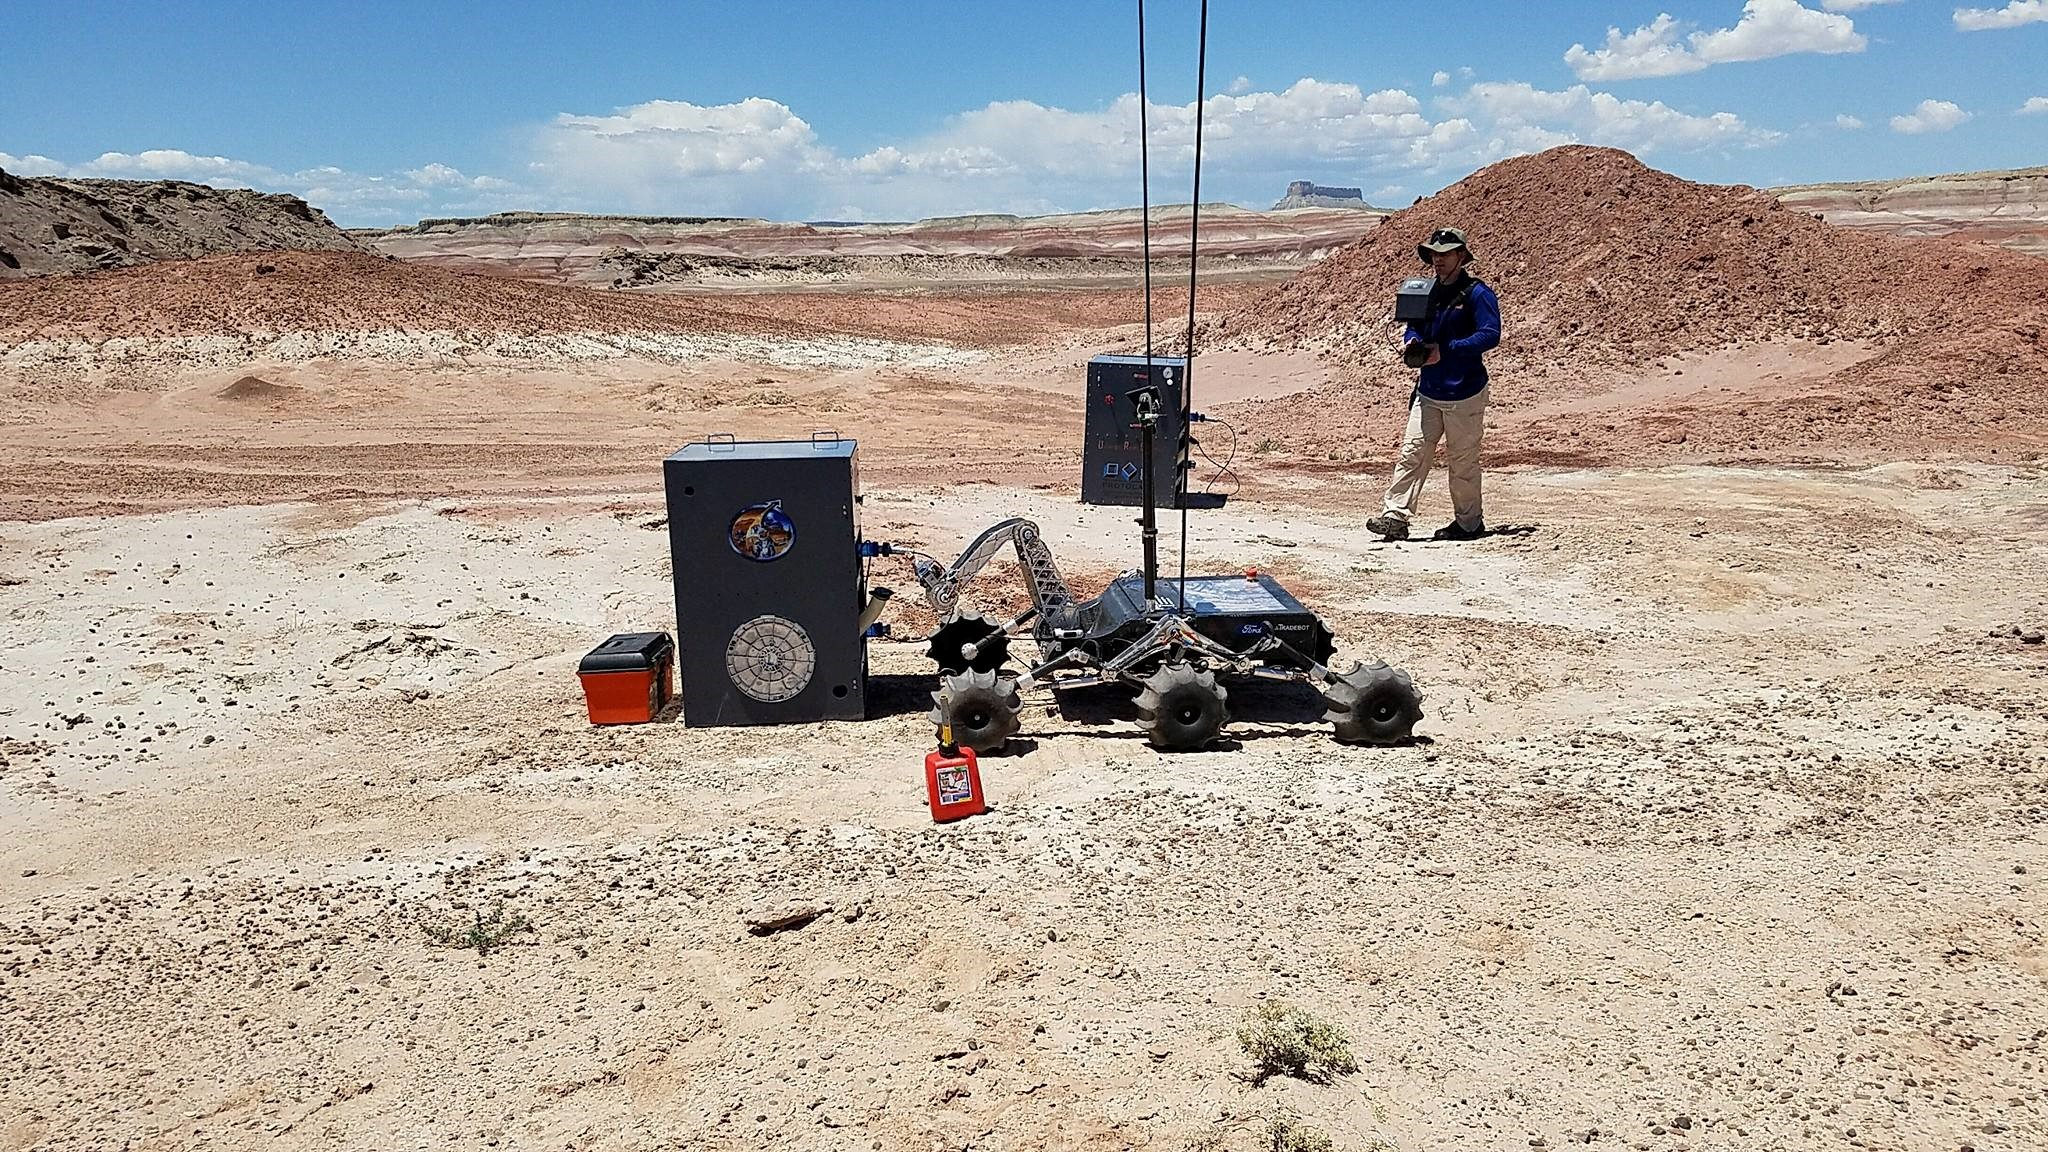
\includegraphics[height=6.2cm]{winning_team}
\caption{A URC competition judge watches as the winning team of 2017, Missouri University of Science and Technology, completes the Equipment Servicing Task.}
\label{fig:winning_team}
\end{figure}

Rovers must be operated remotely by team members who cannot see the rover or communicate with people in the field, such actions are punished by penalty points. Teams must bring and setup their own base station in a provided trailer or shelter and a tall communication mast nearby for wireless communication to the rover. The rover may have to travel up to 1km and even leave direct line of sight to the wireless communication mast. 

The idea is that the rover is on Mars (the Utah desert serves as a substitute) performing scientific experiments and maintenance to a Mars base. An assumption is made that the rovers are being operated by astronauts on or orbiting Mars rather than on Earth and therefore there is no major communication delay. 

\begin{figure}
\centering
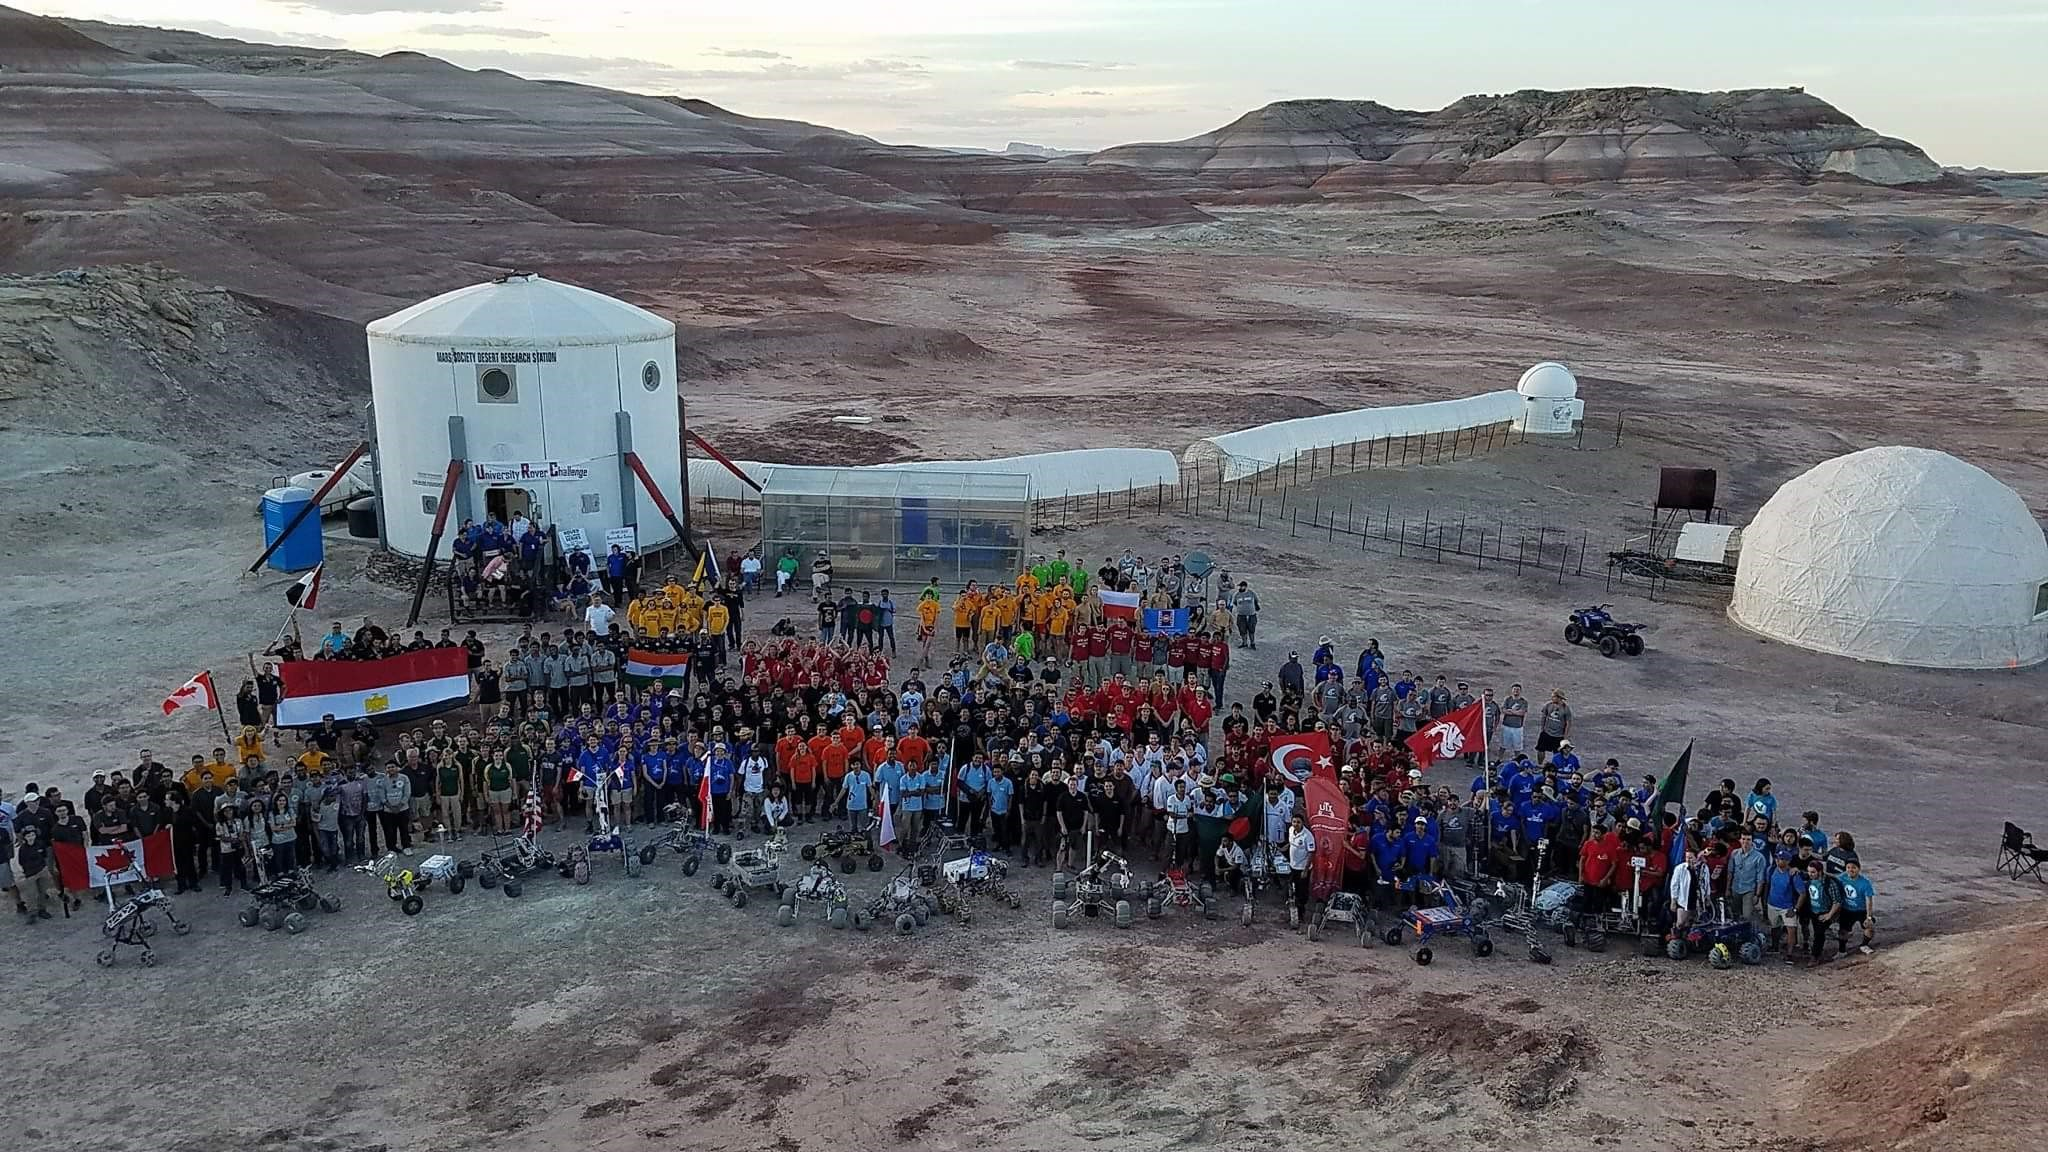
\includegraphics[height=6.2cm]{group_photo}
\caption{Group photo of URC 2017 finalists at the Mars Desert Research Station in Utah.}
\label{fig:group_photo}
\end{figure}

\subsection{University Rover Challenge Tasks}\label{urcrules}
The URC rules\footnote{URC 2017 Rules \url{http://tinyurl.com/urc-rules}} detail four tasks. The science cache task involves retrieving and testing subsurface soil samples without contamination. For this the rover must have an auger to drill into the hard desert soil. After the science task teams present to a panel of judges about their scientific findings. The evidence collected by the rovers cameras, soil collection, and minimum three 3 sensors (e.g. temperature, humidity, pH) is presented in a way that purports the possibility of water and life on Mars.

The extreme retrieval and delivery task requires teams to search out tools and marked rocks in the desert and then use an arm on the rover to bring them back to the base station. The equipment servicing task has teams perform finer manipulations with their rover arm to start a fake generator. This consists of pouring a fuel canister, pressing a button, flicking a switch and more manipulation tasks.

In the autonomous task teams must start with their rover within 2 m of the designated start gate and must autonomously navigate to the finish gate, within 3 m. Teams are provided with GPS coordinates for each gate and the gates are marked with a tennis ball elevated 10 cm to 50 cm off the ground and are not typically observable from a long distance. Teams may conduct teleoperated excursions to preview the course but this will use their time. Total time for this task is 75 minutes per team and the total distance of all stages will not exceed 1000 m.

Teams must formally announce to judges when they are entering autonomous mode and not transmit any commands that would be considered teleoperation, although they can monitor video and telemetry information sent from the rover. On-board systems are required to decide when the rover has reached the finish gate.

The newer 2018 rules\footnote{URC 2018 Rules \url{http://tinyurl.com/urc-rules2018}} are very similar, but with more difficult manipulation tasks such as typing on a keyboard and a more demanding autonomous traversal challenge that explicitly calls for obstacle avoidance–something that Team R3 had last year and is explained in detail in section \ref{r3auto}.

\subsection{Planetary Rovers beyond the Competition}\label{planetary}

Although the University Rover Challenge (URC) competition is a simulation of planetary rovers for Mars, there are significant differences between student built URC rovers and realistic planetary rovers. For example URC teams are limited in budget, manpower and engineering knowledge level, Martian environmental conditions such as radiation, low atmospheric pressure, and very low oxygen levels prompt, and a lack of communication and navigation systems found on Earth such as GPS.

The following paragraphs compare the systems of NASA's Curiosity rover\cite{nasa1}\cite{nasa2} and URC rovers. When comparing the technology difference between the production year of Curiosity (2011) and now should also be kept in mind.

\subsubsection*{On Board Computer (OBC)} The Curiosity Rove carries redundant 200MHz BAE RAD750 CPUs, which is a special CPU that is designed to work in high radiation environments and has 256MB RAM, 2GB Flash, 256KB EEPROM. The CPU is currently running a real time operating system called VxWorks. Interestingly, most of the URC rovers use on board computers that have more features and power than the planetary rovers due to the improvement of technology over the years. For example, Team R3 uses a Jetson TX1, running Ubuntu 16.04 which has 4GB RAM.

\subsubsection*{Autonomous Navigation} Although URC rovers and Curiosity have several common sensors, the lack of GPS leads means that autonomous navigation algorithms work differently. Both of them use their Internal Measurement Units (IMU) and cameras to navigate, combining the odometry from internal sensors, visual odometry and some custom image processing algorithms to reach their target. The difference is that while URC rovers can rely on their GPS to navigate, Curiosity must rely on its position data from internal sensors only. Also, as the Curiosity is navigating on the harsh Mars terrain it decides to navigate through the better terrain using complex image processing algorithms. 

\subsubsection*{Cameras} Curiosity has 17 cameras that are used for various objectives, such as obstacle avoidance, navigation and science. Some of these cameras are very high resolution due to their scientific purposes. URC rovers generally has less cameras, such as 2 or 3 and less resolution is used. 

\subsubsection*{Wireless Communication} Curiosity can communicate directly with the Earth with its X-band (7-12 GHz) communication modules or it can communicate with satellites orbiting Mars, specifically the Mars Reconnaissance Orbiter  (MRO) or Odyssey over a 400MHz UHF link. URC rovers generally prefer a 2.4 GHz UHF link to communicate with their ground stations.

\subsubsection*{Power} Despite most of planetary rovers using solar power, Curiosity carries a 4.8 kg of radioactive plutonium-238 to provide energy to its instruments during its planned mission time of several years. On the other hand, URC rovers are generally powered with Li-Po or Li-Ion batteries that only last for several hours.

\subsection{Prerequisite Skills for Tutorials}

The tutorials in this chapter expect the following skills at a basic level.

\begin{itemize}
\item ROS basics (such as \texttt{roslaunch})
\item Command line basics (such as \texttt{bash})
\item Ubuntu basics (such as \texttt{apt} package manager)
\end{itemize}

\section{Survey of URC Competing Teams}\label{survey}

Fig. \ref{fig:S1} and \ref{fig:S2}  shows eight teams that were surveyed for their rover computer setup, ROS packages, control software, and avionics hardware (for communication, navigation, and monitoring). The team survey results have been edited and condensed for publication.

This survey serves the purpose of providing a broad overview of components and rover development styles before diving into a few detailed implementations in subsequent sections provided by the teams who authored this chapter: Team R3 (Ryerson University), Team Continnuum (University of Wroclaw), and Team ITU (Istanbul Technical University).

Several trends that emerged from the survey are interesting to note. Of the 8 teams surveyed, teams that used Raspberry Pis or STM microcontrollers all placed better than teams that used Arduinos or Teensy microcontrollers. For teleoperator input, Logitech controllers or joysticks were extremely popular and used by all teams. Teams most often expressed difficulty using IMUs or not testing their rover enough. A wide variety of autonomous systems were experimented with: from custom OpenCV implementations, to using existing vision-based obstacle avoidance software (RTAB-Map), to GPS only approaches.

The winning approach of the Mars Rover Design Team from Missouri University of Science and Technology utilized a large number of custom solutions. Their high quality solutions and extremely comprehensive testing is exemplified in just one case by developing a custom UDP communication software. Dubbed "RoveComm", their communication system can reduce latency and increase video quality and was key to successful teleoperation.

\begin{figure}
\centerfloat
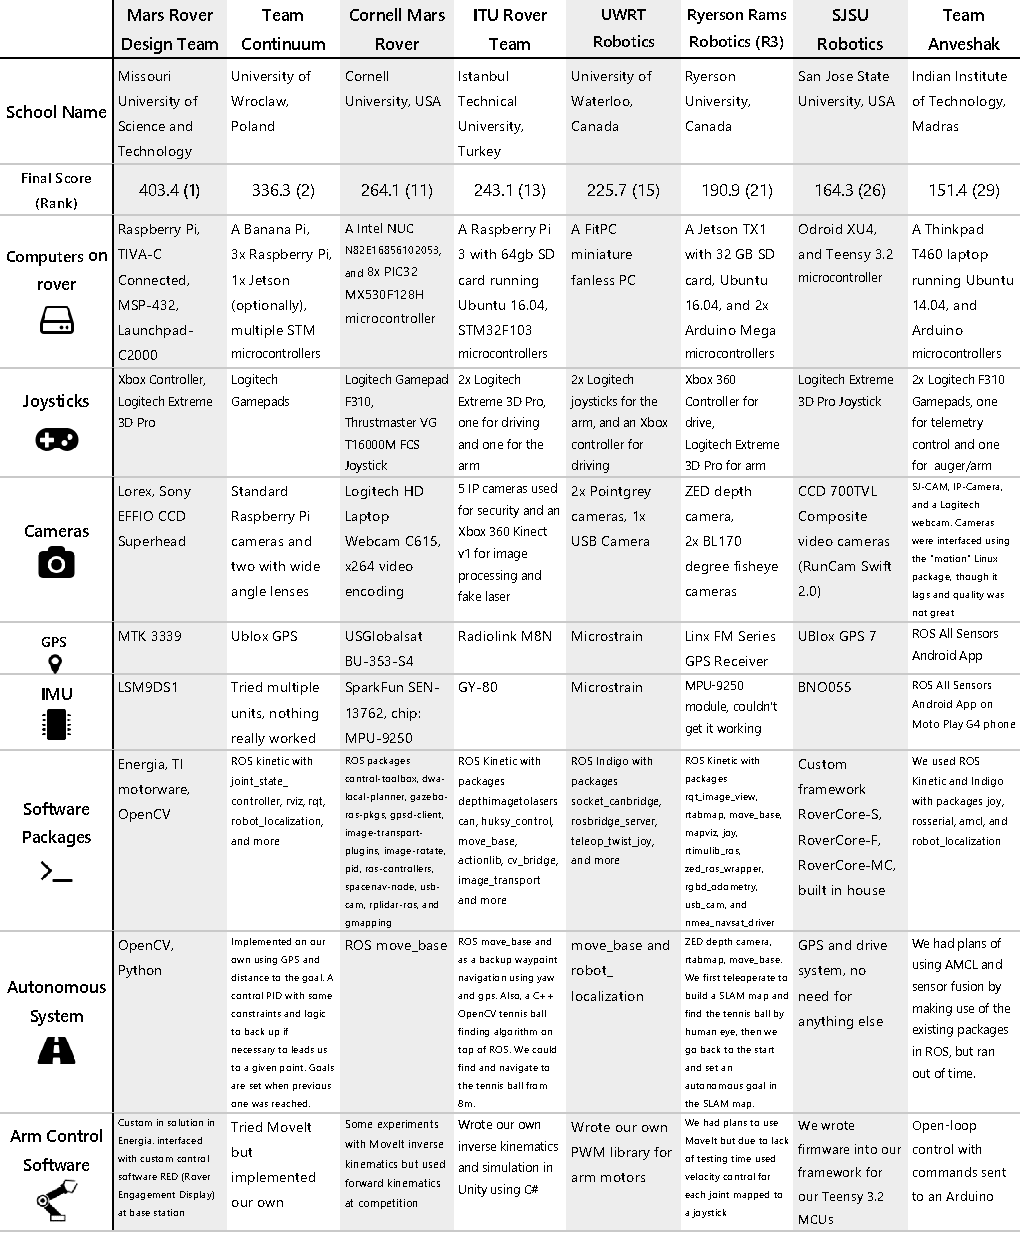
\includegraphics[height=20cm]{surveyP1}
\label{fig:S1}
\caption{Survey of eight rover teams that competed in URC 2017.}
\end{figure}

\begin{figure}
\centerfloat
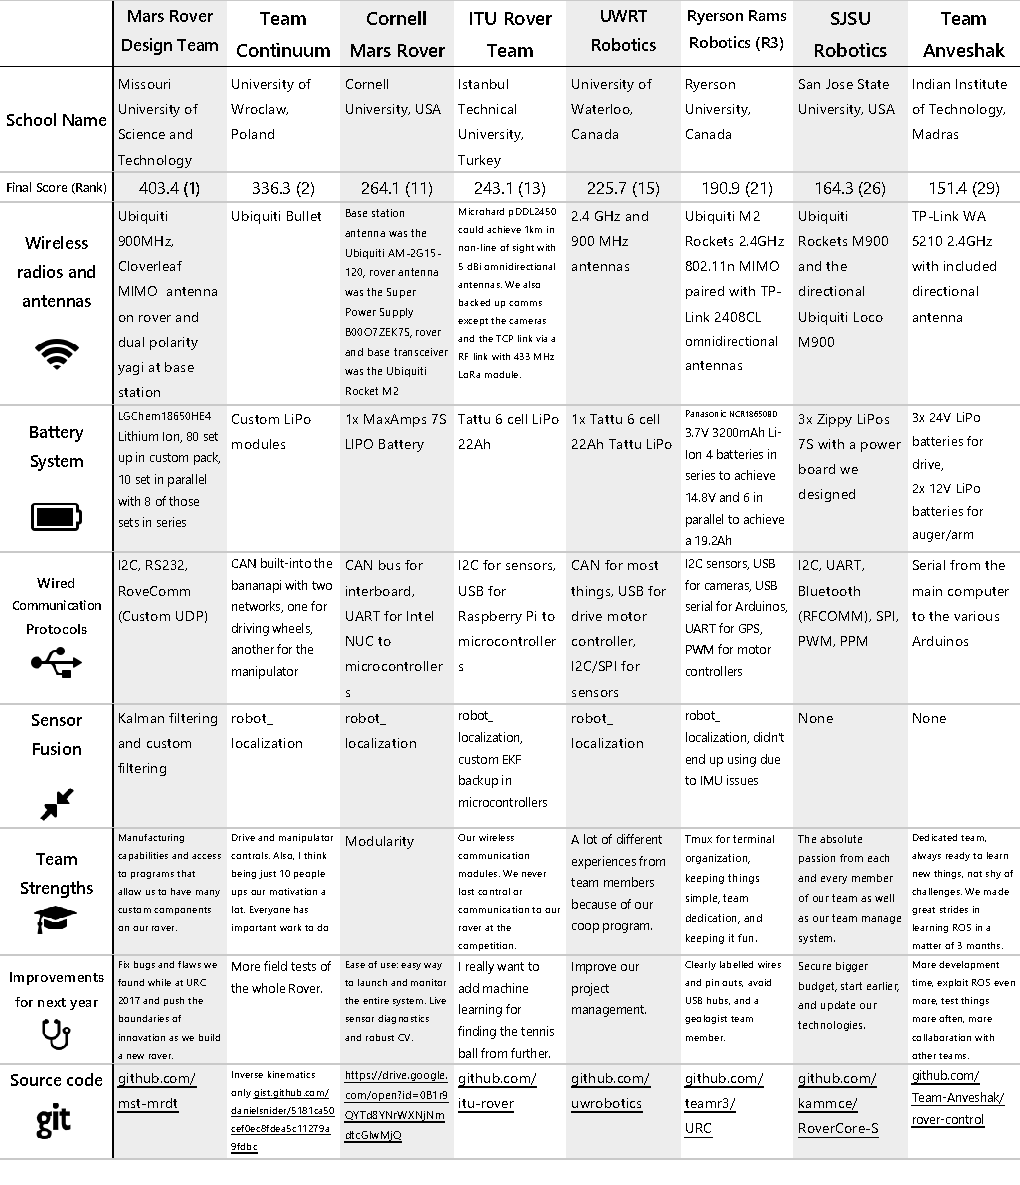
\includegraphics[height=20cm]{surveyP2}
\label{fig:S2}
\caption{Survey of eight rover teams that competed in URC 2017. Cont.}
\end{figure}

\section{Case Study: Continuum Team}\label{continuumcase}

In the following section a case study is presented of the Continuum team (University of Wroclaw) and their rover, Aleph1. It is particularly interesting one, because they managed to score second place during the URC 2017 and had multiple other successes since they debuted in 2015. Michal Barcis decided to share with us some insights about their rover and his opinions on the competition. 

The differences between team Continuum and other participants will be identified in order to find the key strengths that supported their achievements.

\subsection{Recipe for success}
The teams, especially the ones that managed to place themselves in the first ten places during the competition, do not differ very much. Both software and hardware solutions are similar, many teams also decided to implement programs using ROS. We will try to identify some features that distinguish the Continuum team and let the reader decide which of them, if any, were the most advantageous.

One of the key differences is the size of the team. On average there were only around 12 members working on the rover during the period between 2014 and 2017. This makes the Continuum one of the smallest groups on the URC. Such situation has both positive and negative effects – the smaller workforce means each person has more work to do and there is less shared knowledge, but also makes each member more important and increases motivation. Each of the key components in the rover had a person responsible for it. 

There is one especially interesting hardware component that the Continuum team decided to do a bit differently than other teams and the team was often asked about. It is the choice of cameras. Aleph1 is equipped with inexpensive Raspberry Pi cameras\cite{rasppi}. Although much better devices in terms of specification are available on the market, those cameras had a big advantage – it was possible to easily integrate and customize them using raspberry pi. Therefore, it was easy for the team to experiment with different configurations and find a compromise between good quality and low latency. 

The team was also asked what would be one thing they wished to do differently next time and the answer was always the same: more field tests with all components of the rover. This is also the advice that is often given by other teams and it seems very reasonable. By testing the rover with similar tasks as in the competition, it is possible to identify problems sooner and fix them. It also forces the team to complete the work sooner. Unfortunately, to do that properly, a lot of self-control and good organization of the whole group is necessary. 

\subsection{Rover Manipulator Arm }

\begin{figure}
\centering
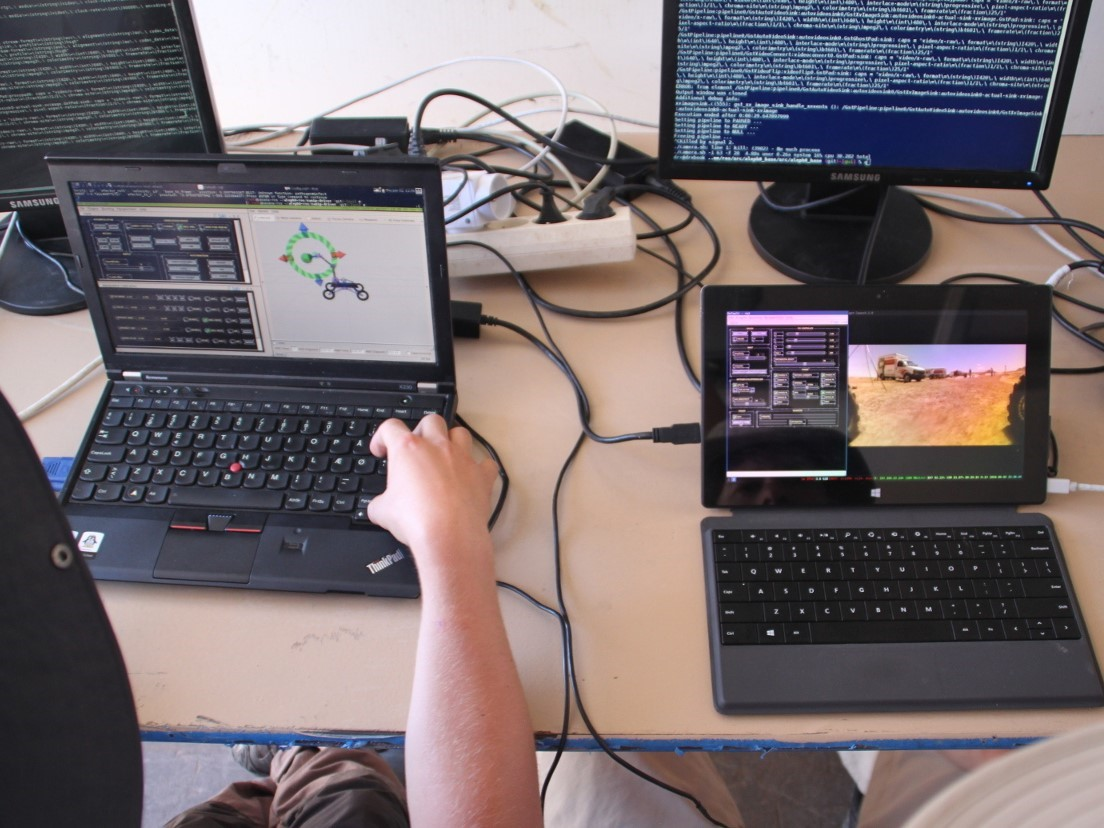
\includegraphics[height=7cm]{contbase}
\caption{Team Continuum's base station setup. A screenshot of their rover control GUI can be seen in \ref{fig:continuumGUI2}}
\label{fig:contbase}
\end{figure}

In the following section, the robotic arm (or "manipulator") of the Aleph1 rover is described. Team Continuum decided to focus on this particular element, because it is crucial in most of the tasks at URC and at the same time is relatively hard to control.

Before starting the work on the arm controller, the Continuum team decided to conduct a survey of currently available solutions of similar problems in ROS. One of the most promising options was the MoveIt! Motion Planning Framework\cite{moveit}. Unfortunately, it was not designed with teleoperation in mind and the team was unable to make it perform reasonably well with a goal specified in real time. Therefore, they have decided to implement their own solution, tailored for the specific hardware they were using. 

The main component that allows the team to control the arm is the inverse kinematics software (python source code\footnote{Continuum Inverse kinematics python source: \url{https://gist.github.com/danielsnider/5181ca50cef0ec8fdea5c11279a9fdbc}}). It utilizes the feedback of four relative encoders placed on the joints of the manipulator to provide the operator two important features: the visualization of the state of the device and the ability to give more intuitive commands to the effector. For example, with this system it is possible to move the gripper up, down, front or back and the speeds of all the motors are automatically adjusted to reach given position.

Another big advantage of the arm system that has proven to be very helpful during the competition is that even when the data connection is not good, it is possible to operate the manipulator. As soon as the instruction reaches the rover, the arm will position itself in the correct way deterministically. This would not be true when using an alternative way of controlling robots where the device is performing some action for as long as a button is being pressed and the loss of packets from the control station might change the result of the operation. Therefore, without such system the operator needs to depend on feedback from cameras which might be delayed or not even available. 

In figures \ref{fig:continuumGUI1}, \ref{fig:continuumGUI2} and \ref{fig:continuumGUI3} the graphical user interface used to control and visualize the state of the manipulator and the whole rover is presented. It is mainly used to support the operator in collision detection and pose estimation, because the visual feedback from the cameras often was not sufficient. The manipulator could be controlled using a mouse, but usually a Logitech game pad was used.

Team Continuum also implemented a semi-automatic system for picking objects up and for flicking manually operated switches. The system was developed for the European Rover Competition (ERC) 2016 because such functionality provided bonus points. Even though it was not deployed during the URC 2017, we have decided to present it in this section, because it is an interesting example of relatively simple extension to the already described system, enabling much more complex tasks.

\begin{figure}
\centering
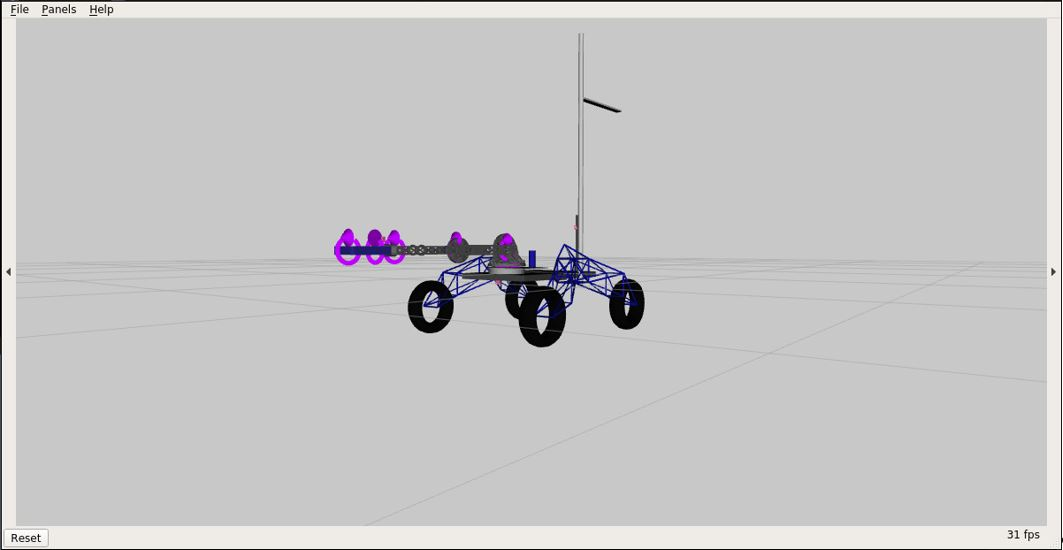
\includegraphics[height=5cm]{continuumGUI1}
\caption{3D visualization of the Aleph1 rover used by the team during teleoperation.}
\label{fig:continuumGUI1}
\end{figure}

\begin{figure}
\centering
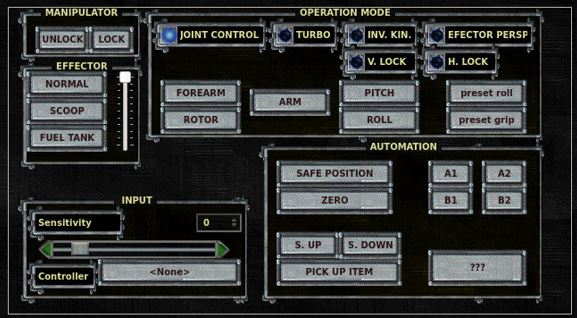
\includegraphics[width=9.2cm]{continuumGUI3}
\caption{Team Continuum's GUI used to control the manipulator of the rover.}
\label{fig:continuumGUI3}
\end{figure}
  
\begin{figure}
\centering
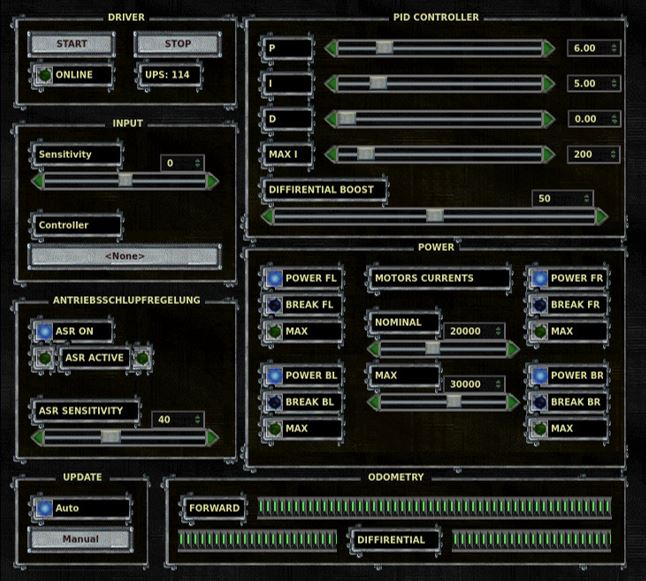
\includegraphics[width=9.2cm]{continuumGUI2}
\caption{Team Continuum's GUI used to control the movements of the rover. }
\label{fig:continuumGUI2}
\end{figure}
 
To get additional points during ERC 2016 the team must have positioned the effector at least 20cm from the object it wanted to pick up or from the two-state switch. Then, the operator should announce he is starting the autonomous mode and put down the controller. Next, the rover should pick up the object or actuate the switch and move back at least 20cm.

The team decided to implement a simple idea: they wanted to place the effector exactly 20cm from the object and directly in front of it. Then, using the inverse kinematics system they were able to execute pre-recorded movements in order to complete the task. 

The first challenge they have faced was how to measure exact distance from objects. They decided to mount two laser pointers on the effector, directed in the direction of each other. They can be seen in multiple scenes of the recently released video\footnote{A recent video of from the University of Wroclaw of their rover has incredible cinematography: \url{https://www.youtube.com/watch?v=MF8DkKDBXtg}} from the University of Wroclaw. The two observable dots meet exactly at 20cm.

The two preprogrammed arm movements were developed as follows:

For flicking switches, the effector went forward for 20cm and 2.5cm down simultaneously, then up for 5cm and back to the initial position (20cm back and 2.5cm down). Due to the mechanical construction and the softness of the end of the arm, Aleph1 was able to switch most of the actuators using this technique, both very small and big ones.

For picking objects up the effector goes down 20cm, then the grip motor engages until the force measurement on this motor crosses a predetermined threshold, then it goes back up 20cm.

The arm of the Aleph1 rover is far from the state of the art manipulators. It is not as fast or precise as it could be and the control sometimes is tricky. However, even though the described solutions might seem simple it was still one of the most advanced robotic arms on URC 2017. It is hard to construct a robust and fail-proof manipulator that is mountable on a movable platform and meets the strict mass and costs limits of URC. The Continuum team has proven that this is possible and the capabilities of such simple platform can be exceptional.

\section{Case Study: Team R3}\label{r3case}
\subsection{ROS Environment}\label{ROS Environment}

\begin{sidewaysfigure}
\centering
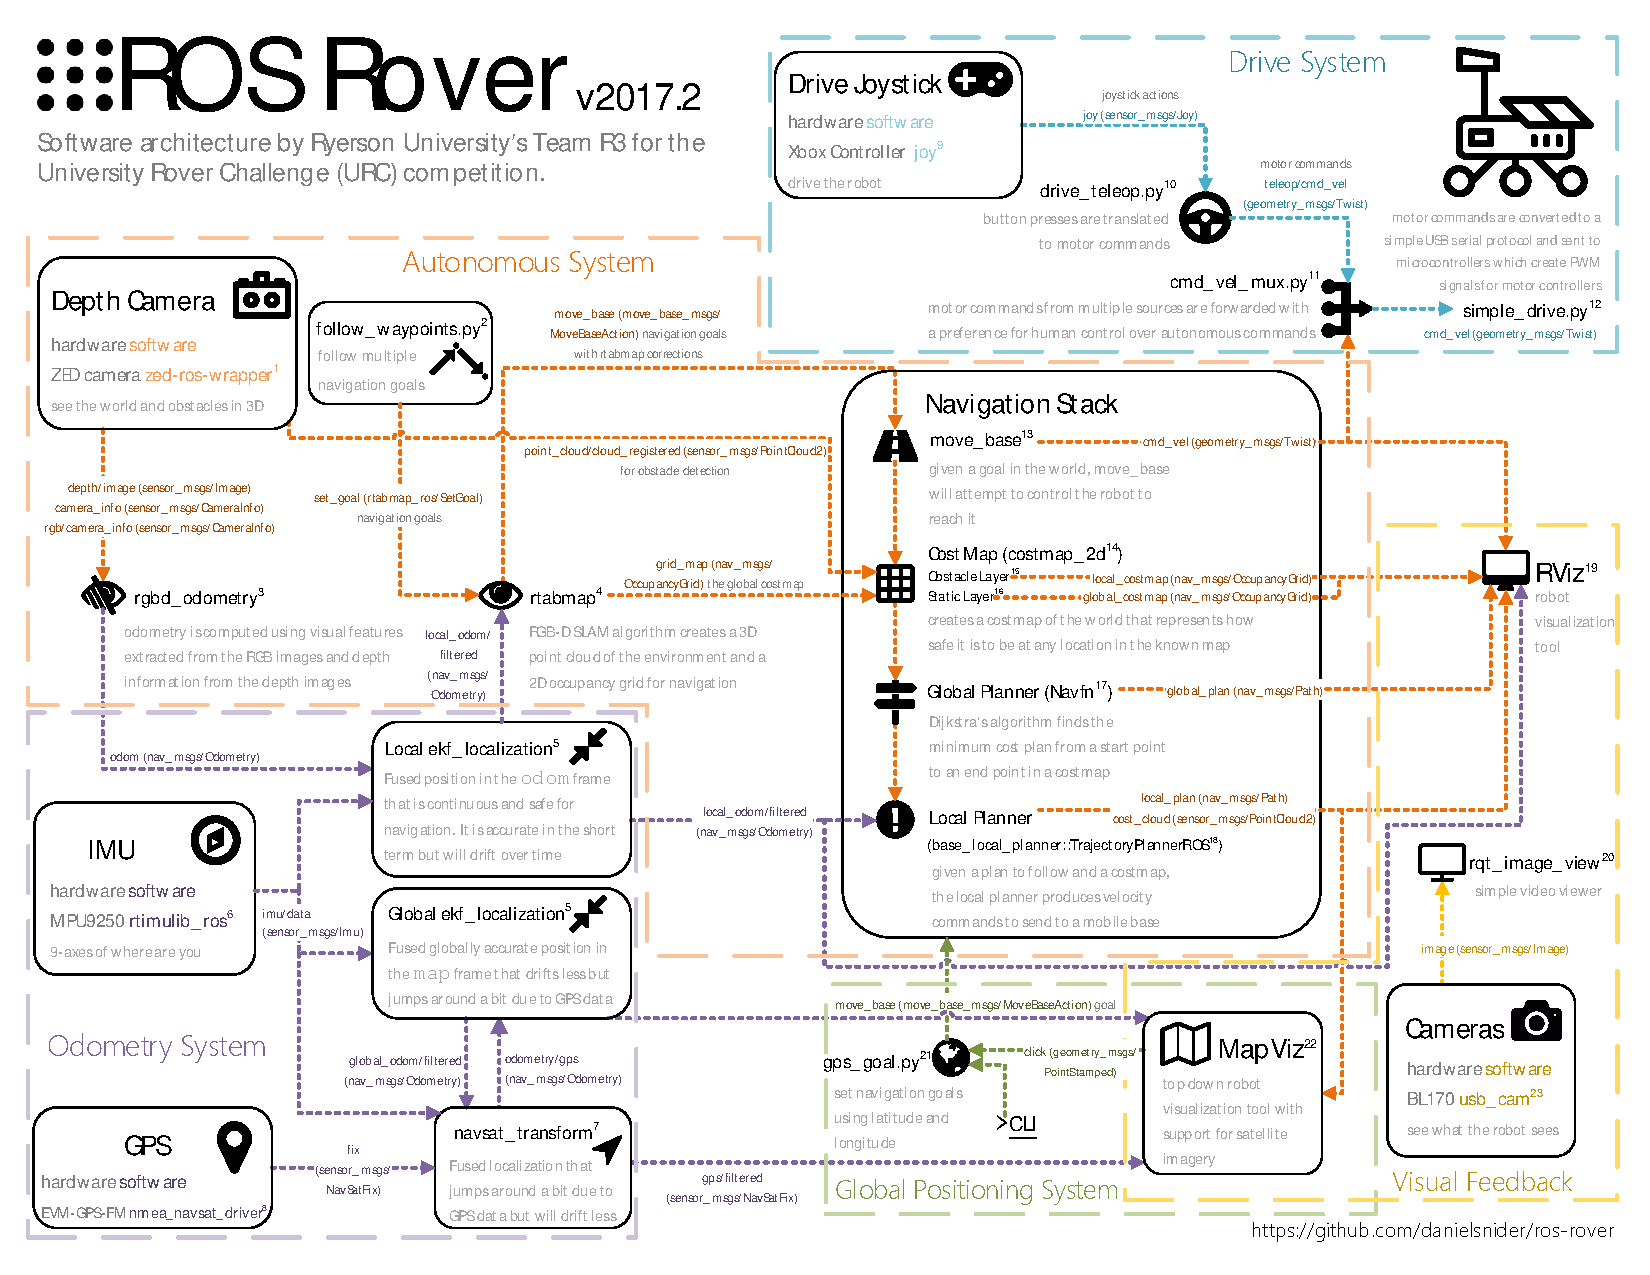
\includegraphics[height=17cm]{Rover_Diagrampdf}
\caption{ROS software architecture of Team R3's rover.}
\label{fig:Diagram}
\end{sidewaysfigure}

At Team R3 (Ryerson University), our Kinetic ROS software built on Ubuntu 16.04 had five main systems: the drive system, the autonomous system, the global positioning system, the visual feedback system, and the odometry system. The full diagram, as seen in Fig. \ref{fig:Diagram}, has been made available in Microsoft Visio format\footnote{Team R3's rover software architecture diagram in Microsoft Visio format \url{https://github.com/danielsnider/ros-rover/blob/master/diagrams/Rover_Diagram.vsdx?raw=true}}.

To learn more about each software component, links to the most relevant documentation are provided.

\subsubsection*{Autonomous System}
Team R3's autonomous system consists of the ZED depth camera and the RTAB-Map ROS package for SLAM mapping\cite{labbe2014online}. The authors have also contributed gps\_goal and follow\_waypoints ROS packages for added goal setting convenience. For further details about the autonomous system see the tutorial in section \ref{r3auto}.

\begin{lstlisting}[frame=single,caption={Autonomous system software used in Team R3's rover (numbers refer to Fig. \ref{fig:Diagram}).},basicstyle=\sffamily\scriptsize]
1. zed-ros-wrapper (http://wiki.ros.org/zed-ros-wrapper)
2. follow_waypoints.py (http://wiki.ros.org/follow_waypoints)
3. rgbd_odometry (http://wiki.ros.org/rtabmap_ros#rgbd_odometry)
4. rtabmap (http://wiki.ros.org/rtabmap_ros)
21. gps_goal.py (http://wiki.ros.org/gps_goal)
\end{lstlisting}

\subsubsection*{Odometry System}\label{odomsys}
At the URC competition teams are surrounded by sandy desert terrain in Utah. As a result of wheel slippage on sand, Team R3 did not use wheel odometry. Instead we focused on fusing IMU and visual odometry into a more reliable position and orientation. However, because our IMU was not working well enough to produce a good fused result, at the competition we did not actually use the ekf\_localization\cite{MooreStouchKeneralizedEkf2014} ROS nodes of the odometry system. Instead we relied on odemetry from the rgbd\_odometry ROS node only and this worked well for our autonomous system based on the RTAB-Map package.

\begin{lstlisting}[frame=single,caption={Odometry software components used in Team R3's rover (numbers refer to Fig. \ref{fig:Diagram}).},basicstyle=\sffamily\scriptsize]
5. ekf_localization (http://docs.ros.org/kinetic/api/robot_localization/html/)
6. rtimulib_ros (https://github.com/romainreignier/rtimulib_ros)
7. navsat_transform (http://docs.ros.org/kinetic/api/robot_localization/html/)
8. nmea_navsat_driver (http://wiki.ros.org/nmea_navsat_driver)
\end{lstlisting}


\subsubsection*{Drive System}
The drive software created by Team R3 is called simple\_drive because it does not produce wheel odometry or transforms. That is left to the autonomous system via SLAM and is more robust in slippery desert environments. The simple\_drive package controls 6 motors with PWM pulses using an Arduino dedicated to driving. For further details of the drive system see the tutorial in section \ref{drive}.

\begin{lstlisting}[frame=single,caption={Drive system software used in Team R3's rover (numbers refer to Fig. \ref{fig:Diagram}).},basicstyle=\sffamily\scriptsize]
9. joy (http://wiki.ros.org/joy)
10. drive_teleop.py (http://wiki.ros.org/simple_drive#drive_teleop)
11. cmd_vel_mux.py (http://wiki.ros.org/simple_drive#cmd_vel_mux)
12. simple_drive.py (http://wiki.ros.org/simple_drive#simple_drive-1)
\end{lstlisting}

\subsubsection*{Navigation Stack}
The navigation stack used by Team R3 follows the commonly used development patterns of the ROS navigation stack\footnote{ROS Nagivation stack \url{http://wiki.ros.org/navigation}}. Our setting choices were inspired by RTAB-Map's tutorial\footnote{RTAB-Map tutorial for the ROS navigation stack \url{http://wiki.ros.org/rtabmap_ros/Tutorials/StereoOutdoorNavigation}} and we share our tips in section \ref{r3auto}.

\begin{lstlisting}[frame=single,caption={ Navigation software stack used in Team R3's rover (numbers refer to Fig. \ref{fig:Diagram}).},basicstyle=\sffamily\scriptsize]
13. move_base (http://wiki.ros.org/move_base)
14. Cost Map costmap_2d (http://wiki.ros.org/costmap_2d)
15. Cost Map Obstacle Layer (http://wiki.ros.org/costmap_2d/hydro/obstacles)
16. Cost Map Static Layer (http://wiki.ros.org/costmap_2d/hydro/staticmap)
17. Global Planner Navfn (http://wiki.ros.org/navfn)
18. Local Planner base_local_planner (http://wiki.ros.org/base_local_planner)
\end{lstlisting}

\subsubsection*{Visual Feedback}
To assist in teleoperation of the robot, sensors and navigation plans were visualized in rviz for local information such as point clouds and in mapviz for a global context that includes satellite imagery. The visual feedback software and joystick software was executed remotely on a laptop in the control station. The rest of software was executed on a Jetson TX1 inside the rover.

\begin{lstlisting}[frame=single,caption={Visual feedback software used by Team R3 (numbers refer to Fig. \ref{fig:Diagram}).},basicstyle=\sffamily\scriptsize]
19. RViz (http://wiki.ros.org/rviz)
20. rqt_image_view (http://wiki.ros.org/rqt_image_view)
22. MapViz (http://wiki.ros.org/mapviz)
23. usb_cam (http://wiki.ros.org/usb_cam)
\end{lstlisting}

\section{Tutorial: Autonomous Waypoint Following}\label{waypoint}

The following tutorial documents an original ROS package follow\_waypoints\footnote{Source code for follow\_waypoints ROS package \url{https://github.com/danielsnider/follow_waypoints}}\footnote{Wiki page for follow\_waypoints ROS package \url{http://wiki.ros.org/follow_waypoints}} that will buffer move\_base goals until instructed to navigate to them in sequence. If you can autonomously navigate from A to B, then you can combine multiple steps of A to B to form more complicated paths and use cases. For example, do you want your rover to take the scenic route? Are you trying to reach your goal and come back? Do you need groceries on the way home from Mars?

\afterpage{
\begin{figure}
\centering
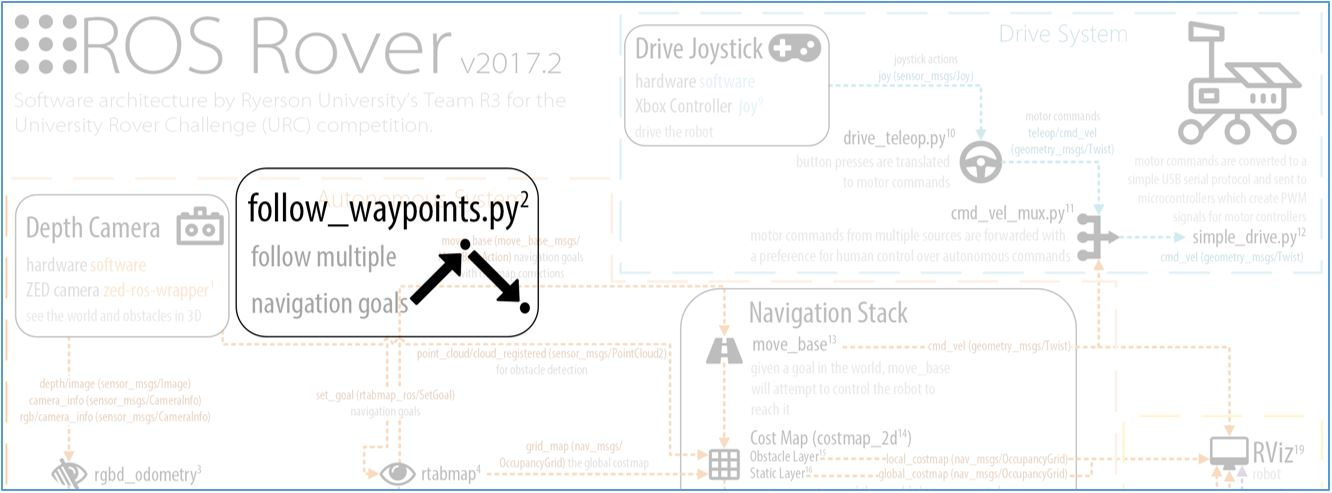
\includegraphics[width=\textwidth]{waypoints}
\caption{ROS node follow\_waypoints as seen in the larger architecture diagram. See Fig. \ref{fig:Diagram} for the full diagram.}
\label{fig:waypoints}
\end{figure}
}

Team R3 (Ryeson Univerisity) has developed the follow\_waypoints ROS package to use actionlib to send the goals to move\_base in a robust way. The code structure of follow\_waypoints.py is a barebones state machine. For this reason it is easy to add complex behavior controlled by state transitions. For modifying the script to be an easy task, you should learn about the Python state machine library in ROS called SMACH\footnote{SMACH state machine library for python \url{http://wiki.ros.org/smach}}\footnote{One alternative to SMACH is py-trees, a behavior tree library \url{http://py-trees.readthedocs.io/en/devel/background.html}}. The state transitions in the script occur in the order \texttt{GET\_PATH} (buffers goals into a path list), \texttt{FOLLOW\_PATH}, and \texttt{PATH\_COMPLETE} and then they repeat.

\begin{figure}
\centering
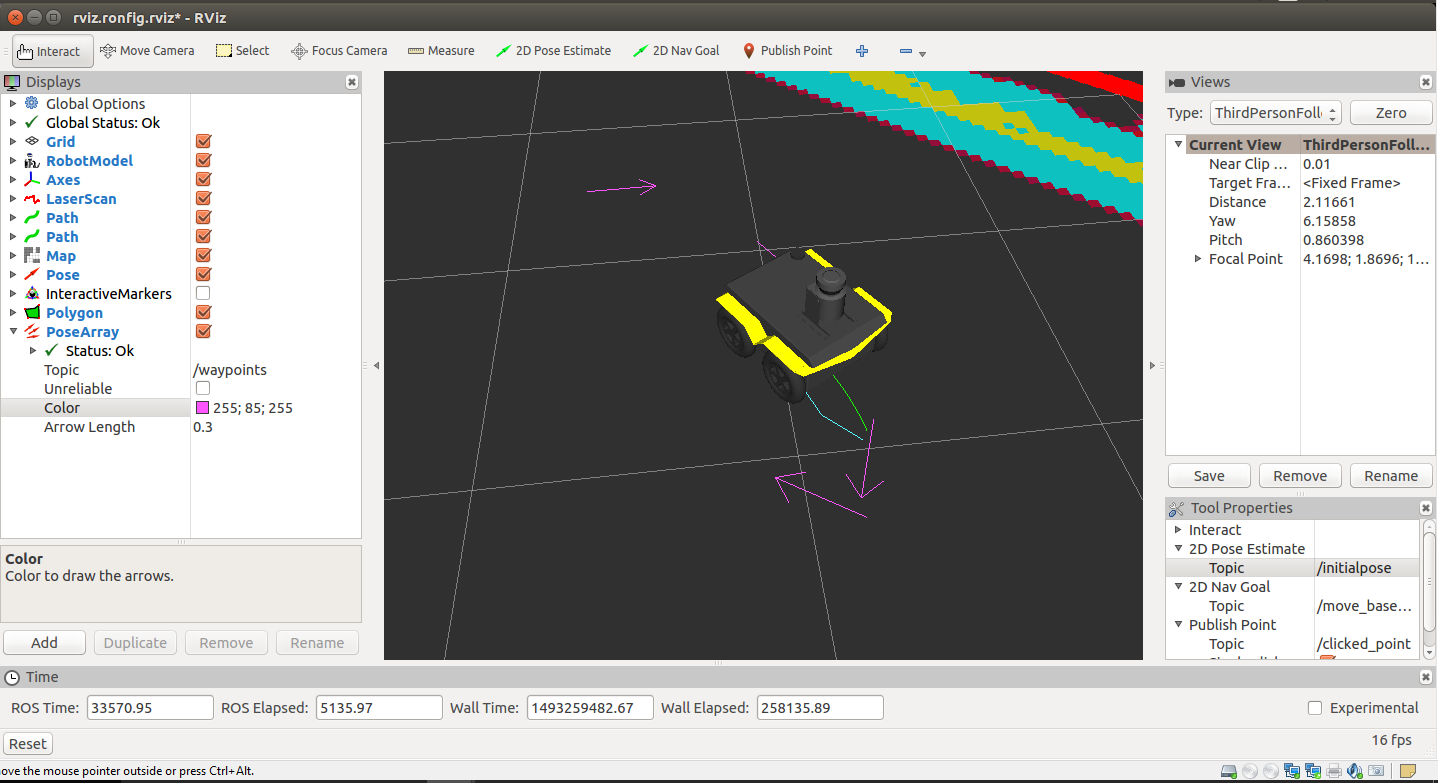
\includegraphics[width=\textwidth]{waypoints2}
\caption{A simulated Clearpath Jackal robot\protect\footnotemark navigating to one of several waypoints displayed as pink arrows.}
\label{fig:waypoints2}
\end{figure}
\footnotetext{Clearpath Jackal tutorials for Ubuntu 14.04 \url{http://docs.ros.org/indigo/api/jackal_tutorials/html/simulation.html}}

\subsection{Usage in the University Rover Challenge (URC)}
A big advantage of waypoint following is that the rover can go to points beyond reachable by Wi-Fi. In the autonomous traversal task, Team ITU's rover at one point lost connection but then got it back again when it reached the waypoint.

Other possible uses of waypoint following: To navigate to multiple goals in the autonomous task with a single command (use in combination with GPS goals, see Section \ref{gpsnav}). To search a variety of locations, ideally faster than by teleoperation. To allow for human assisted obstacle avoidance where an obstacle is known to fail detection.

\subsection{Usage Instructions}

1. Install the ROS package:

\begin{lstlisting}[frame=single,basicstyle=\ttfamily\footnotesize]
$ sudo apt-get install ros-kinetic-follow-waypoints
\end{lstlisting}

\noindent 2. Launch the ROS node:

\begin{lstlisting}[frame=single,basicstyle=\ttfamily\footnotesize]
$ roslaunch follow_waypoints follow_waypoints.launch
\end{lstlisting}

\noindent  3. To set waypoints you can either publish a ROS Pose message to the /initialpose topic directly or use RViz's tool "2D Pose Estimate" to click anywhere. Fig. \ref{fig:waypoints2} shows the pink arrows representing the current waypoints in RViz. To visualize the waypoints in this way, use the topic /current\_waypoints, published by follow\_waypoints.py as a PoseAarray type.\\

\noindent 4. To initiate waypoint following send a "path ready" message.

\begin{lstlisting}[frame=single,basicstyle=\ttfamily\footnotesize]
$ rostopic pub /path_ready std_msgs/Empty -1
\end{lstlisting}

\noindent To cancel the goals do the following. This is the normal move\_base command to cancel all goals.

\begin{lstlisting}[frame=single,basicstyle=\ttfamily\footnotesize]
$ rostopic pub -1 /move_base/cancel actionlib_msgs/GoalID -- {}
\end{lstlisting}

\subsection{Normal Output}
When you launch and use the follow\_waypoints ROS node you will see the following console output. 

\begin{lstlisting}[frame=single,basicstyle=\ttfamily\scriptsize,breaklines=true]
$ roslaunch follow_waypoints follow_waypoints.py

[INFO] : State machine starting in initial state 'GET_PATH' with userdata: ['waypoints']
[INFO] : Waiting to receive waypoints via Pose msg on topic /initialpose
[INFO] : To start following waypoints: 'rostopic pub /path_ready std_msgs/Empty -1'
[INFO] : To cancel the goal: 'rostopic pub -1 /move_base/cancel actionlib_msgs/GoalID -- {}'
[INFO] : Received new waypoint
[INFO] : Received new waypoint
[INFO] : Received path ready message
[INFO] : State machine transitioning 'GET_PATH':'success'-->'FOLLOW_PATH'
[INFO] : Executing move_base goal to position (x,y): 0.0123248100281, -0.0620594024658
[INFO] : Executing move_base goal to position (x,y): -0.0924506187439, -0.0527720451355
[INFO] : State machine transitioning 'FOLLOW_PATH':'success'-->'PATH_COMPLETE'
[INFO] : ###############################
[INFO] : ##### REACHED FINISH GATE #####
[INFO] : ###############################
[INFO] : State machine transitioning 'PATH_COMPLETE':'success'-->'GET_PATH'
[INFO] : Waiting to receive waypoints via Pose msg on topic /initialpose 
\end{lstlisting}


\section{Tutorial: Image Overlay Scale and Compass}\label{overlay}

In an effort to add context about of the world to imagery recorded, Team R3 has developed a ROS package image\_overlay\_compass\_and\_scale\footnote{Source code for the image\_overlay\_compass\_and\_scale ROS package \url{https://github.com/danielsnider/image_overlay_scale_and_compass}}\footnote{Wiki page for the image\_overlay\_compass\_and\_scale ROS package \url{http://wiki.ros.org/image_overlay_scale_and_compass}} that can add an indication of scale and compass to images and video streams. A compass graphic will be embedded into imagery in a way that makes north direction apparent. A scale bar is also added so that the size of objects in images is more easily interpreted. 

Compass and scale values must be provided using standard ROS Float32 messages. Alternatively, a command interface can be used without ROS. 

This tool meets one of the requirements of URC 2017 (in an automated way) and is applied to images of soil sampling sites and scenic panoramas for scientific and geological purposes.

This package uses the OpenCV\cite{opencv_library} python library to overlay a compass graphic, the scale bar and dynamic text which is set using a ROS topic.

The implementation of overlaying the compass graphic on the input image follows these steps: 1) resize the compass graphic to be 60\% the size of the input image's smaller side (whichever is smaller, x or y resolution). 2) Rotate the compass to the degrees specified on the /heading input topic. 3) Warp the compass to make it appear that the arrow is pointing into the image. This assumes that the input image has a view forward facing with the sky in the upper region of the image.

\begin{figure}
\centering
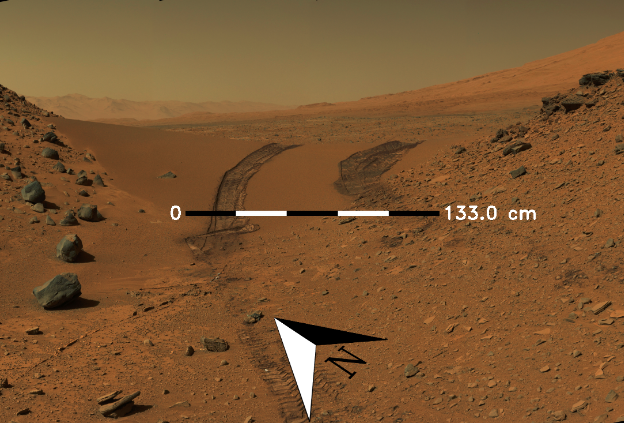
\includegraphics[width=0.8\textwidth]{overlay1}
\caption{Example of the image\_overlay\_compass\_and\_scale ROS package.}
\label{fig:overlay1}
\end{figure}

\subsection{Usage Instructions}

1. Install the ROS package:

\begin{lstlisting}[frame=single,basicstyle=\ttfamily\footnotesize,breaklines=true]
$ sudo apt-get install ros-kinetic-image-overlay-compass-and-scale
\end{lstlisting}

\noindent 2. Launch the ROS node:

\begin{lstlisting}[frame=single,basicstyle=\ttfamily\footnotesize,breaklines=true]
$ roslaunch image_overlay_compass_and_scale overlay.launch
\end{lstlisting}

\noindent 3. Publish heading and scale values

\begin{lstlisting}[frame=single,basicstyle=\ttfamily\footnotesize,breaklines=true]
$ rostopic pub /heading std_msgs/Float32 45 # unit is degrees
$ rostopic pub /scale std_msgs/Float32 133 # unit is centimeters 
\end{lstlisting}

\noindent 4. View resulting image

\begin{lstlisting}[frame=single,basicstyle=\ttfamily\footnotesize]
$ rqt_image_view /overlay/compressed
\end{lstlisting}

\begin{figure}
\centering
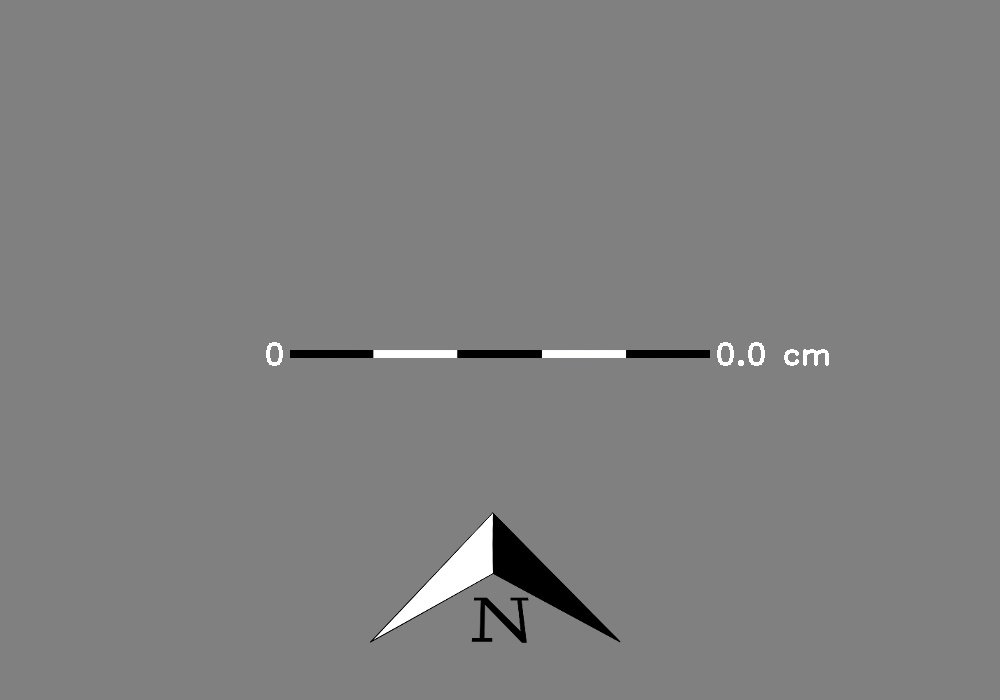
\includegraphics[width=0.8\textwidth]{overlay2}
\caption{This is what to expect when nothing is received by the node. This is the default published image.}
\label{fig:overlay2}
\end{figure}


\subsection{Command Line Interface (CLI)}

The image\_overlay\_compass\_and\_scale ROS package includes a command line interface to invoke the program once and output and image with the overlayed graphics.

\begin{lstlisting}[frame=single,basicstyle=\ttfamily\footnotesize,breaklines=true,caption={Example usage of the image\_overlay\_compass\_and\_scale CLI script to save the image overlay to disk instead of publishing to ROS.}]
$ roscd image_overlay_compass_and_scale
$ ./src/image_overlay_compass_and_scale/image_overlay.py --input-image ~/mars.png --heading 45 --scale-text 133 --output-file output.png
\end{lstlisting}

\section{Tutorial: A Simple Drive Software Stack}\label{drive}

The authors have published a new ROS package, simple\_drive\footnote{Source code for simple\_drive ROS package \url{https://github.com/danielsnider/simple_drive}}\footnote{Wiki page for simple\_drive ROS package \url{http://wiki.ros.org/simple_drive}}, used at the University Rover Challenge (URC) 2017 on Team R3's rover. It proved simple and effective in desert conditions. The package is simple in the sense that it does not publish TF odometry from wheel encoders because on sand wheels slip very substantially.

The package implements skid steering joystick teleoperation with three drive speeds, dedicated left and right thumbsticks control left and right wheel speeds, control of a single axis panning servo to look around the robot, a cmd\_vel multiplexer to support a coexisting autonomous drive system, and Arduino firmware to talk to PWM motors and a servo. For the sake of simplicity, this package does not do the following: TF publishing of transforms, wheel odometry publishing, PID control loop, no URDF, or integration with ros\_control. Though all of these simplifications are normal best practices in sophisticated robots. The simple\_drive package gives ROS users the ability advance their robot more quickly and hopefully to find more time to implement best practices.

This package is divided into four parts: drive\_teleop ROS node, cmd\_vel\_mux ROS node, simple\_drive ROS node, drive\_firmware Arduino code. In the following sections we will explain the main features and implementation details but for the full ROS API documentation please see the simple\_drive online ROS wiki.

\begin{figure}
\centering
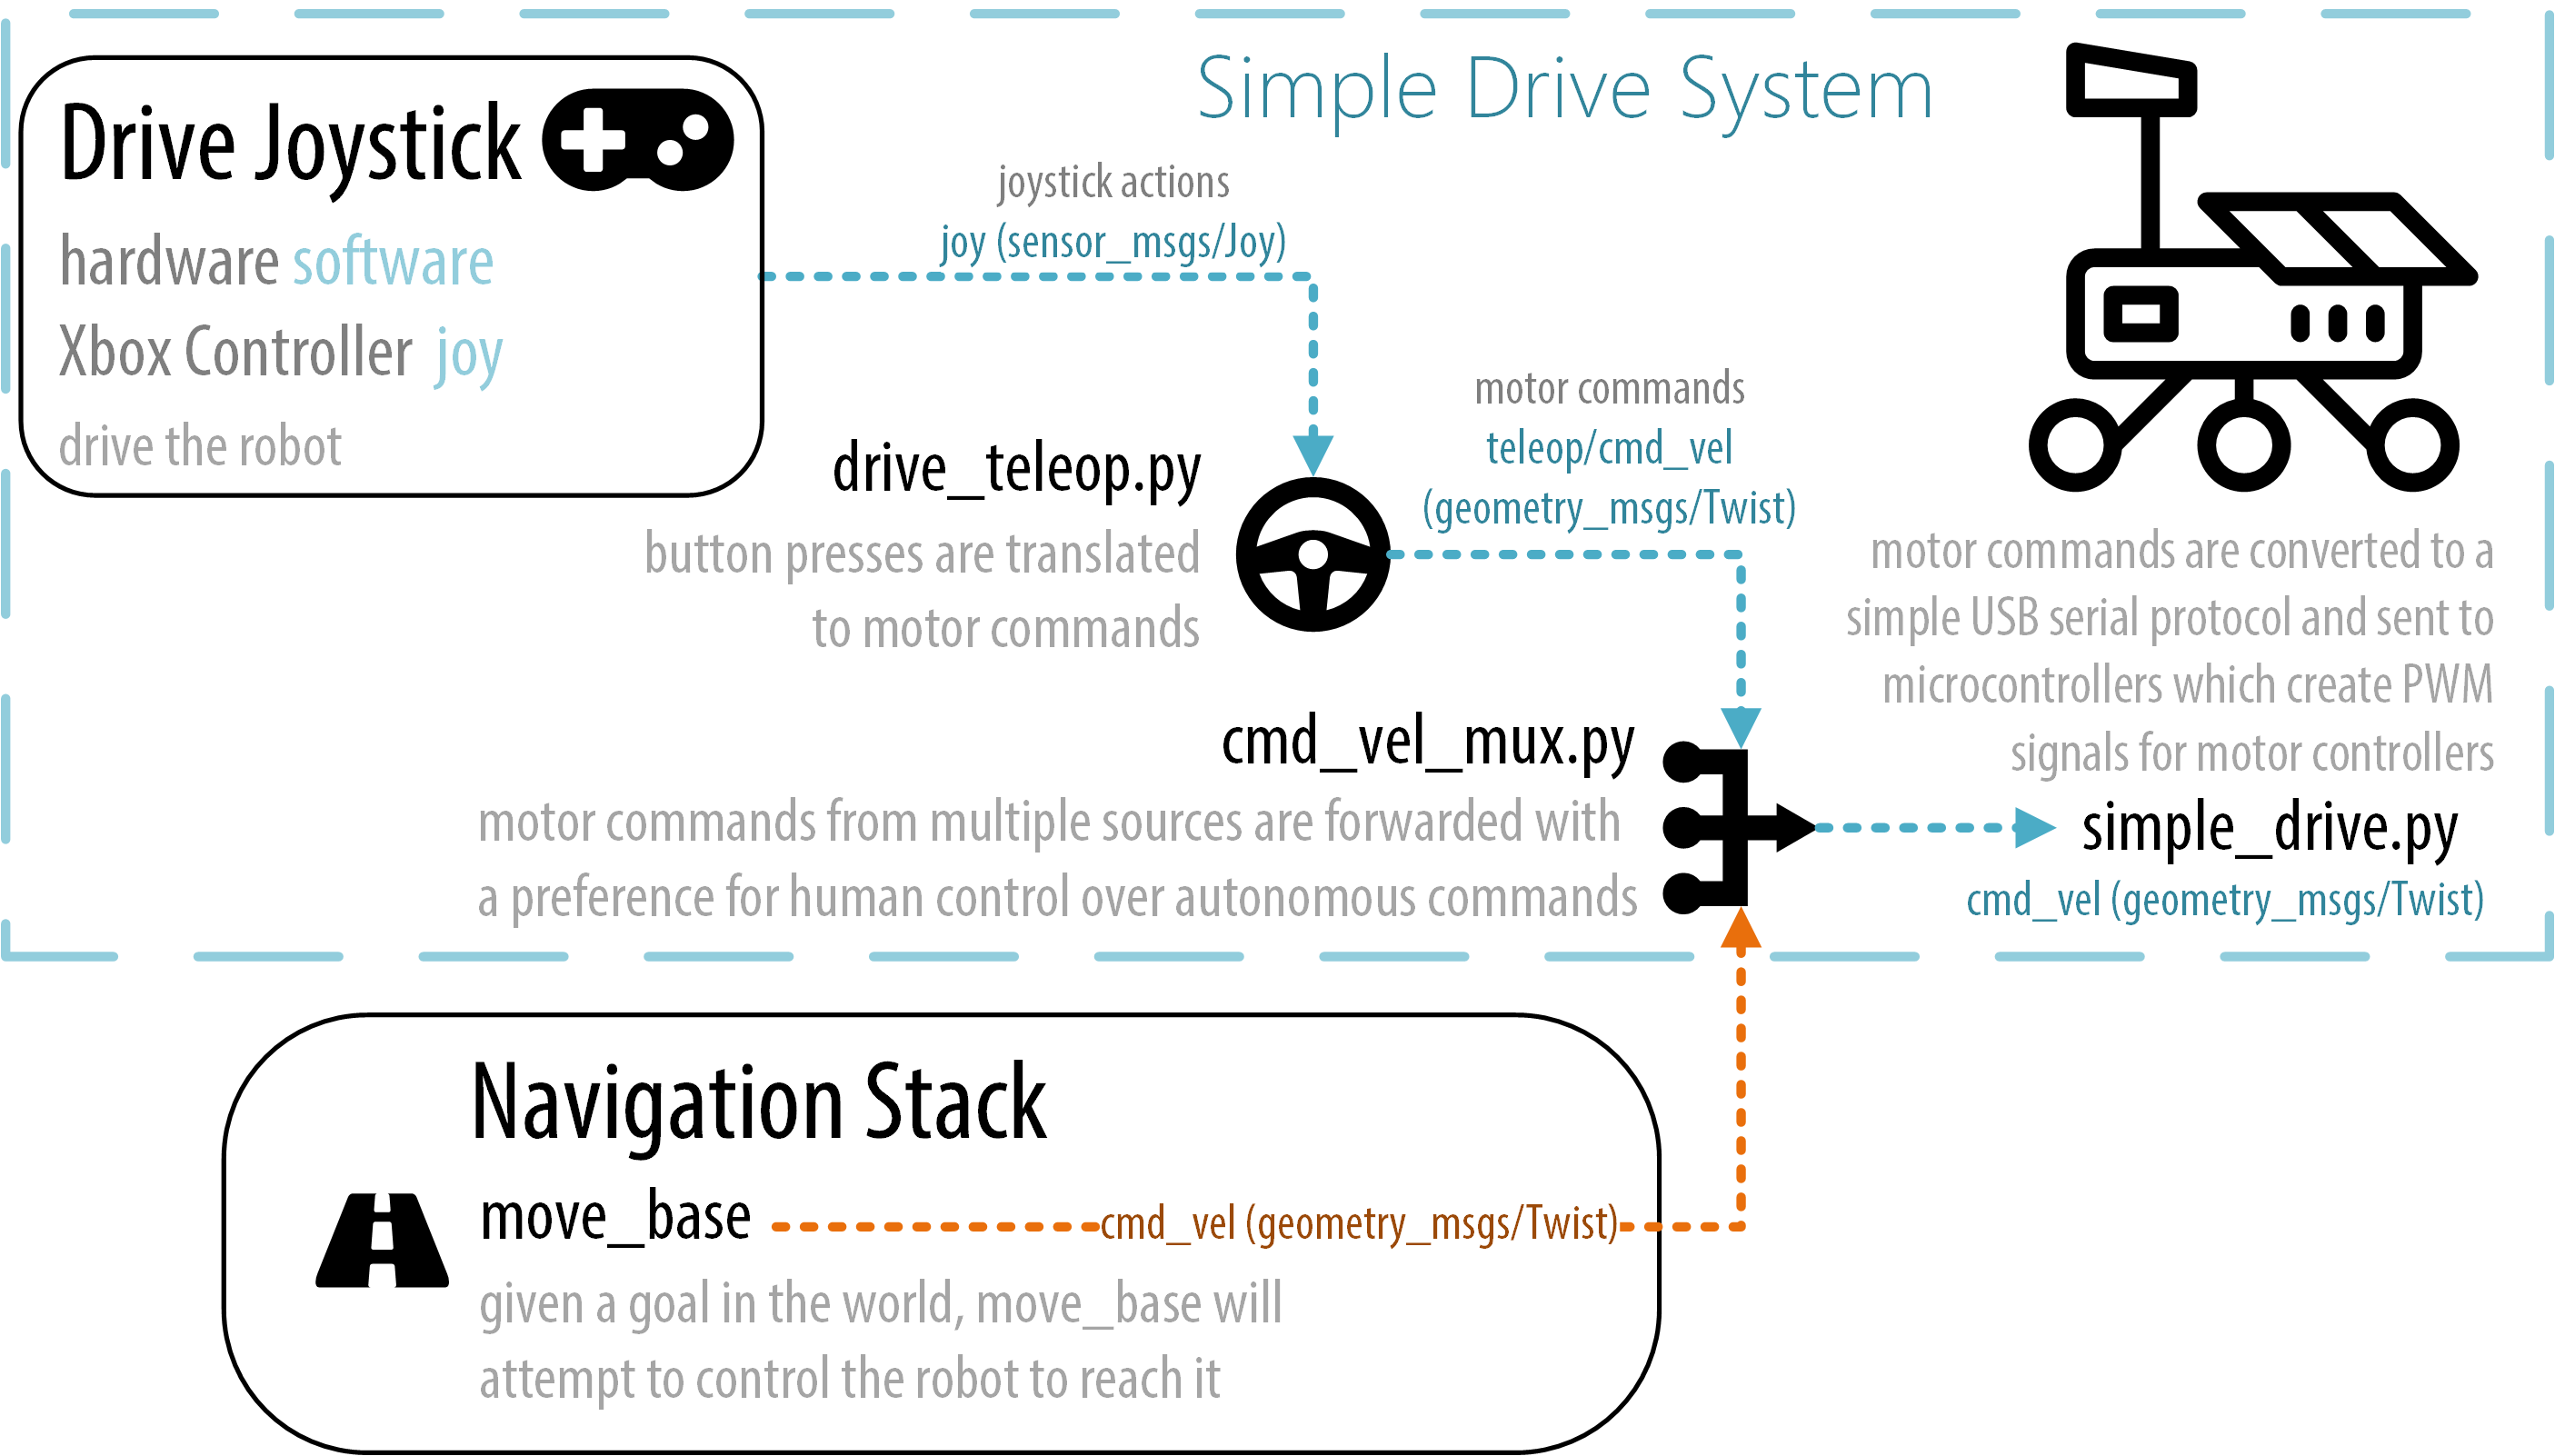
\includegraphics[width=\textwidth]{Simple_Drive_Diagram}
\caption{Architecture of the drive ROS software used by Team R3. See fig. \ref{fig:Diagram} for a larger diagram. Note that the drive\_firmware microcontroller software component is not illustrated but it useful to note that it communicates with simple\_drive.py.}
\label{fig:Simple_Drive_Diagram}
\end{figure}

\begin{figure}
\centering
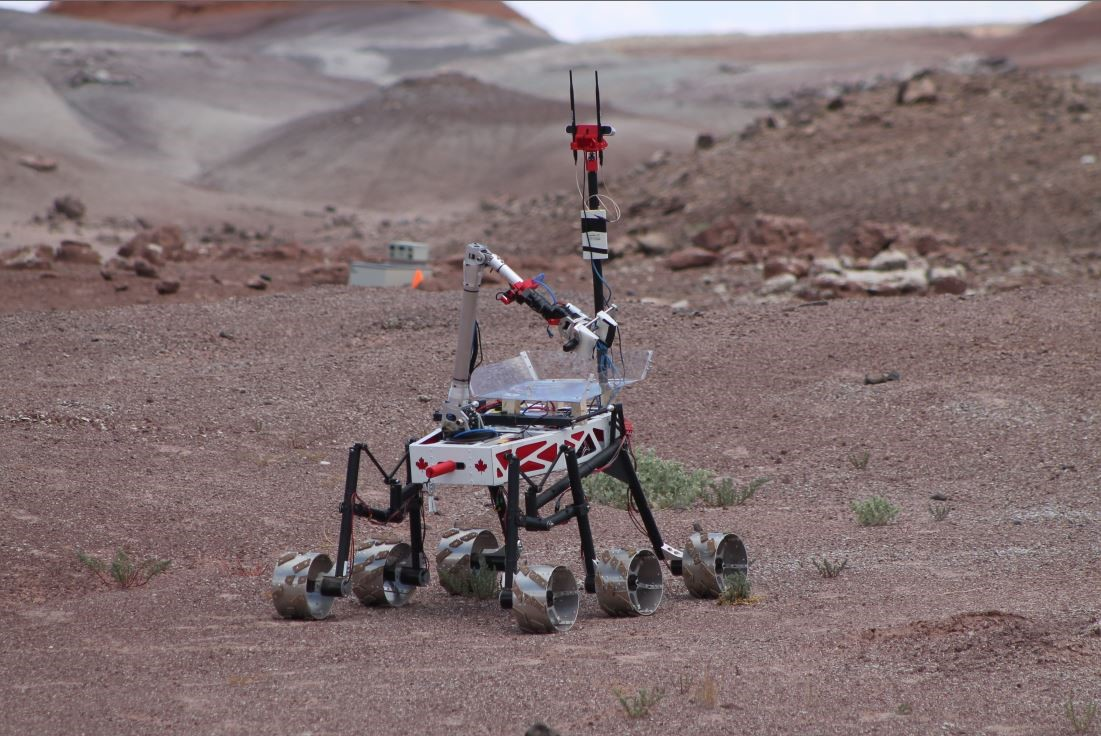
\includegraphics[width=11cm]{rover_simple_drive}
\caption{Team R3's rover being teleoperated by the simple\_drive ROS package.}
\label{fig:rover_simple_drive}
\end{figure}

\subsection{Usage Instructions}

1. Install the ROS package:
\begin{lstlisting}[frame=single,basicstyle=\ttfamily\footnotesize]
$ sudo apt-get install ros-kinetic-simple-drive
\end{lstlisting}

\noindent 2. Install the drive\_firmware onto a microcontroller connected to your motors and wheels by PWM. See section \ref{drive_firmware} for detailed instructions. The microcontroller must also be connected to the computer running the simple\_drive ROS node by a serial connection (e.g. USB).

\noindent 3. Launch the three simple\_drive ROS nodes separately or together using the included \texttt{drive.launch} file:
\begin{lstlisting}[frame=single,basicstyle=\ttfamily\footnotesize]
$ roslaunch simple_drive drive_teleop.launch joy_dev:=/dev/input/js0
$ roslaunch simple_drive cmd_vel_mux.launch
$ roslaunch simple_drive simple_drive.launch serial_dev:=/dev/ttyACM0
# OR all-in-one launch
$ roslaunch simple_drive drive.launch
\end{lstlisting}

\noindent 4. Your robot should now ready to be driven.

\subsection{drive\_teleop ROS Node}

The drive\_teleop node handles joystick input commands and outputs desired drive speeds to the cmd\_vel\_mux ROS Node. This node handles joystick inputs in a in skid steering style, also known as diff drive or tank drive where the left joystick thumbstick controls the left wheels and the right thumbstick controls the right wheels. We refer to this layout as tank drive through this section.

\begin{figure}[H]
\centering
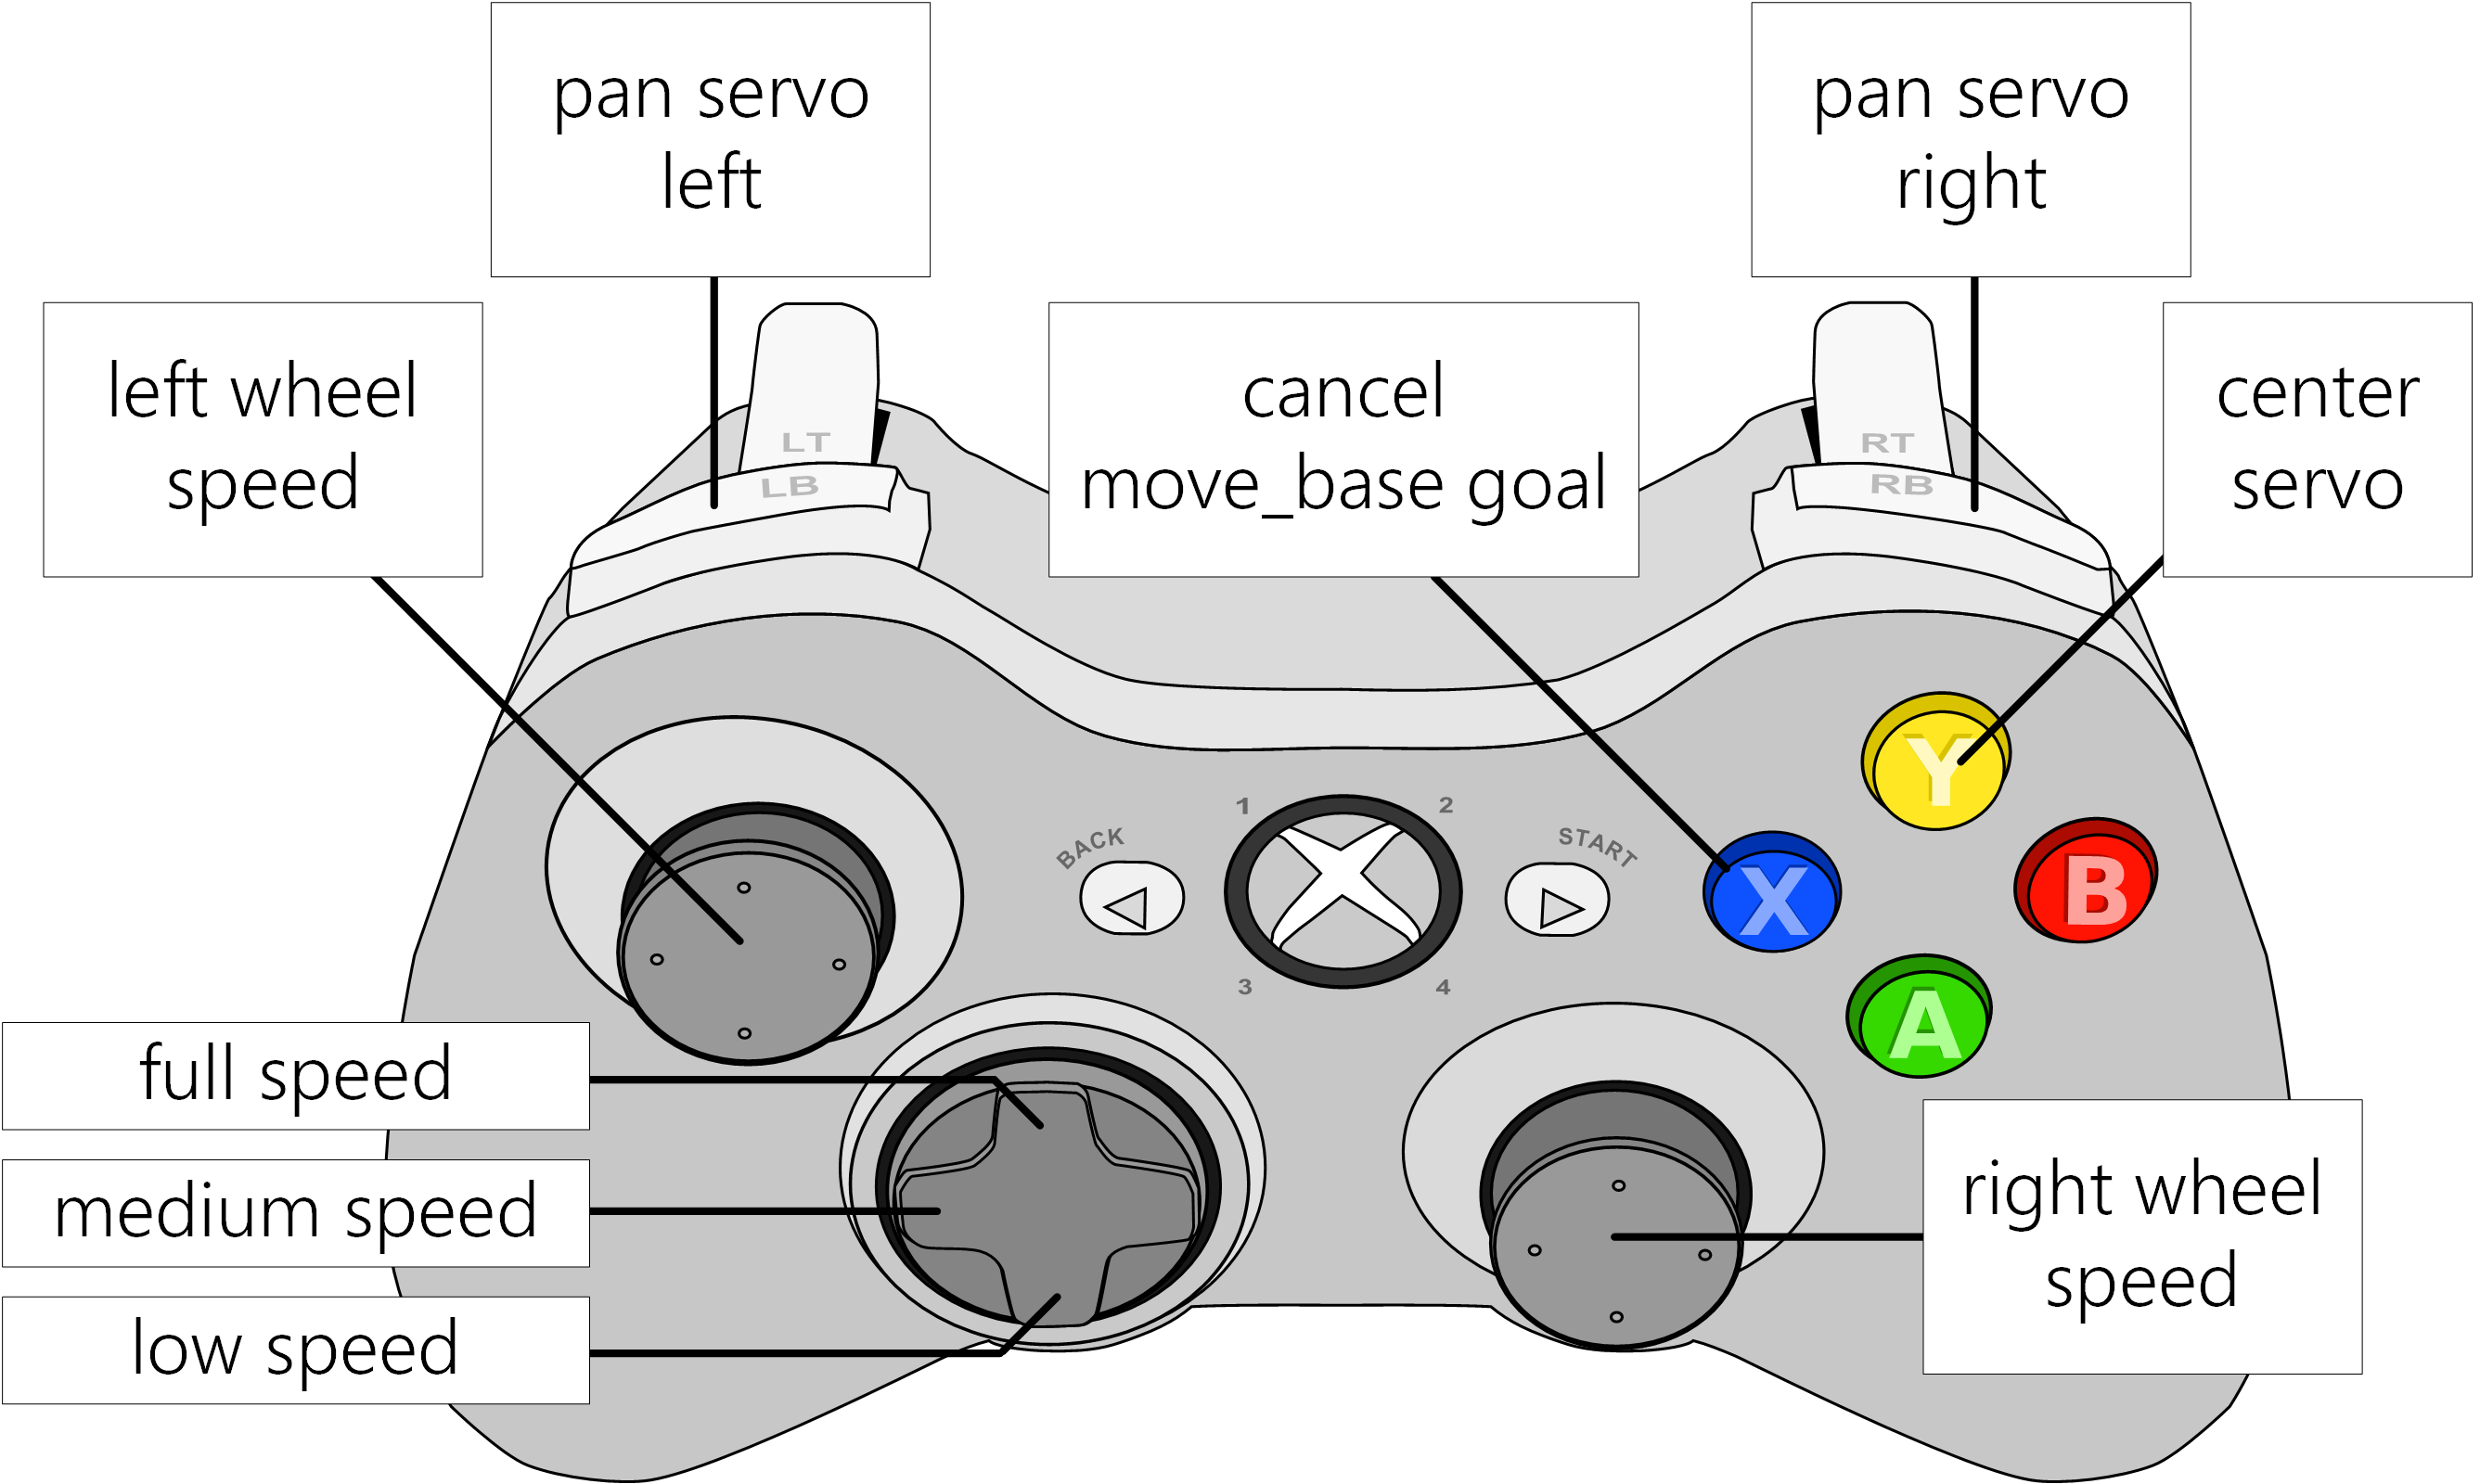
\includegraphics[width=9.2cm]{simple_drive_Xbox_Controller}
\caption{The Xbox 360 joystick button layout for the simple\_drive package (diagram is available in Visio format\protect\footnotemark). Image credit: Microsoft Corporation}
\label{fig:simple_drive_Xbox_Controller}
\end{figure}

\footnotetext{Xbox 360 joystick button layout diagram in Visio format \url{https://github.com/danielsnider/ros-rover/blob/master/diagrams/simple_drive_Xbox_Controller.vsdx?raw=true}}

More specifically, this node converts sensor\_msgs/Joy messages from the joy ROS node into geometry\_msgs/Twist messages which represent the desired drive speed. Listing \ref{fig:simple_drive_Xbox_Controller} shows that there are programmed buttons to set the drive speed to low, medium, or high speed, look around with a single axis servo, and cancel move\_base goals at any moment. 

Typically the servo is used to move a camera so that the teleoperator pan around the surroundings of the robot. The servo's rotation speed (in degrees per button press) can be set using the \texttt{servo\_pan\_speed} ROS parameter. The minimum and maximum angle of servo rotation in degrees can be set using the \texttt{servo\_pan\_min} and \texttt{servo\_pan\_max} ROS parameters respectively.

The button mapping was tested on an Xbox 360 controller and should require little or no modification for similar controllers, if they support a DirectInput mode.

\subsection{cmd\_vel\_mux ROS Node}

The cmd\_vel\_mux node receives movement commands on two sensor\_msgs/Twist topics, one for teleoperation and one for autonomous control, typically move\_base. Movement commands are multiplexed (i.e. forwarded) to a final topic for robot consumption with a preference for human control over autonomous commands. If any teleoperation movement command is received the cmd\_vel\_mux node will block autonomous movement commands for a set time defined by the \texttt{block\_duration} ROS parameter.

\subsection{simple\_drive ROS Node}

The simple\_drive node sends commands to motors by communicating with a microcontroller over serial using the protocol defined by the drive\_firmware. The simple\_drive node listens to geometry\_msgs/Twist for motor commands and std\_msgs/Float32 for the servo position. The serial device that simple\_drive communicates with is set with the \texttt{serial\_dev} and \texttt{baudrate} ROS parameters.

This node is very simple and could be eliminated if your microcontroller supports ROS. For example Arduinos can use rosserial\_arduino. However, this node is written in Python so you could more easily add complex functionality in Python and then in your microcontroller do the minimum amount of work necessary allowing for the use of smaller and more lightweight microcontrollers.

\subsection{drive\_firmware Ardiuno Software}\label{drive_firmware}

The drive\_firmware is software for an Arduino microcontroller and it does not run as a ROS node. The Arduino is assumed to be dedicated to use of the simple\_drive package. It does the minimum amount of work possible to receive motor commands from the simple\_drive node over a USB serial connection and output voltages to digital PWM output to be received by motor controllers.

We tested on an Arduino Mega 2560 and Arduino Due, however many other boards should work with the same code and setup steps thanks to PlatformIO. You may need to change to change the pin numbers. Note that this software does not stop moving the robot if no messages are received, or if communications are lost.

\subsubsection*{Serial Communication Protocol}\label{serproto} The drive\_firmware uses a serial protocol that is designed for simplicity rather than integrity of messages. As such it should not be perceived as especially robust. However, it has worked consistently in our experience. 

Fig. \ref{fig:drive_protocol} shows how data is encoded over the serial connection. A header command byte is transmitted followed by one or two (depending on the command) IEEE 754 standard binary float values. Linear and angular velocity are expected to be between -1 and 1, which are linearly scaled to motor duty-cycles by the drive\_firmware.

\begin{figure}[H]
\centering
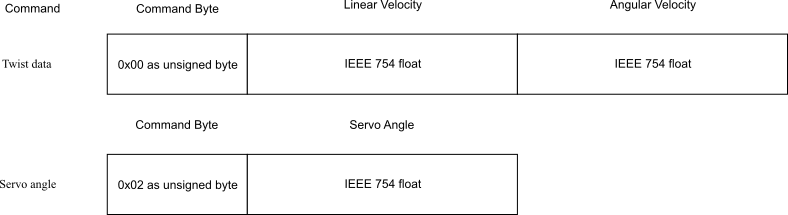
\includegraphics[width=\textwidth]{drive_protocol}
\caption{Diagram of the serial format used by drive\_firmware to communicate between microcontroller and an on board computer.}
\label{fig:drive_protocol}
\end{figure}

An example packet following this format could be encoded as bytes: 0x00 0x3f 0x80 0x00 0x00 0x00 0x00 0x00 0x00. This would be decoded as a twist data (leading 0x00) with 1.0 for linear velocity (0x3f 0x80 0x00 0x00) and 0.0 for angular velocity (0x00 0x00 0x00 0x00).


\subsubsection*{Tank to Twist Calculation} When left and right joystick inputs are received by the drive\_teleop node, representing left and right wheel linear velocities\footnote{Wheel linear velocity is meant to be the speed at which distance is travelled and not rpm.} (i.e. skid steering or differential drive), a conversion calculation to a geometry\_msgs/Twist with linear and rotational velocities is performed as seen in equations \ref{linvel} and \ref{angvel}. The parameter \(r\) is the half of the distance between your rover's wheels in meters.

\begin{equation}\label{linvel}
Linear\ Velocity\ (\frac{m}{s})=\frac{left\_velocity + right\_velocity}{2.0}
\end{equation}

\begin{equation}\label{angvel}
Angular\ Velocity\ (\frac{rad}{s})=\frac{left\_velocity - right\_velocity}{2.0 \times r}
\end{equation}

\subsubsection*{Twist to Tank Calculation}

When a geometry\_msgs/Twist containing linear and rotational velocities is received by the drive\_firmware, corresponding linear velocities are calculated for the left and right sides of wheel banks on the vehicle as seen in equation \ref{leftvel} and \ref{rightvel}.

\begin{equation}\label{leftvel}
Left\ Side\ Linear\ Velocity\ (\frac{m}{s})=linear\_velocity + angular\_velocity \times r
\end{equation}

\begin{equation}\label{rightvel}
Right\ Side\ Linear\ Velocity\ (\frac{m}{s})=linear\_velocity - angular\_velocity \times r
\end{equation}

\subsubsection*{PlatformIO} We deploy the drive\_firmware to an Arduino microcontroller using PlatformIO\footnote{PlatformIO is an open source ecosystem for IoT development \url{http://platformio.org/}} because it allows for a single source code to be deployed to multiple platforms. PlatformIO supports approximately 200 embedded boards and all major development platforms such as Atmel, ARM, STM32 and more.

\subsection{Install and configure drive\_firmware}

The following steps demonstrate how to install and configure drive\_firmware component of the simple\_drive package. These steps were tested on Ubuntu 16.04.

\noindent 1. Install PlatformIO\footnote{More information on how to install PlatformIO is here \url{http://docs.platformio.org/en/latest/installation.html#super-quick-mac-linux}}:

\begin{lstlisting}[frame=single,basicstyle=\ttfamily\footnotesize]
$ sudo python -c "$(curl -fsSL https://raw.githubusercontent.com/platformio/platformio/master/scripts/get-platformio.py)"
# Enable Access to Serial Ports (USB/UART)
$ sudo usermod -a -G dialout <your username here>
$ curl https://raw.githubusercontent.com/platformio/platformio/develop/scripts/99-platformio-udev.rules  > /etc/udev/rules.d/99-platformio-udev.rules
# After this file is installed, physically unplug and reconnect your board.
$ sudo service udev restart
\end{lstlisting}


\noindent 2. Create a PlatformIO project\footnote{More documentation about PlatformIO: \url{http://docs.platformio.org/en/latest/quickstart.html}}:

\begin{lstlisting}[frame=single,basicstyle=\ttfamily\footnotesize]
$ roscd simple_drive
$ cd ./drive_firmware/
# Find the microcontroller that you have in the list of PlatformIO boards
$ pio boards | grep mega2560
# Use the name of your board to initialize your project
$ pio init --board megaatmega2560
\end{lstlisting}


\noindent 3. Modify the microcontroller pin layout to match wirings to motor controller hardware. First open the file containing the pin settings then change the pin numbers as needed:

\begin{lstlisting}[frame=single,basicstyle=\ttfamily\footnotesize]
$ vim src/main.cpp +4

   1 // Pins to Left Wheels
   2 #define pinL1 13
   3 #define pinL2 12
   4 #define pinL3 11
   5 // Pins to Right Wheels
   6 #define pinR1 9
   7 #define pinR2 8
   8 #define pinR3 7
   9 // Pin to the Servo
  10 #define pinServo 5
\end{lstlisting}

\noindent 4. Depending on the specs of your motor controllers, modify the PWM settings as needed (values are duty-cycles in microseconds):

\begin{lstlisting}[frame=single,basicstyle=\ttfamily\footnotesize]
$ vim src/main.cpp +17

   1 // PWM specs of the Spark motor controller. Spark manual:
   2 //      http://www.revrobotics.com/content/docs/LK-ATFF-SXAO-UM.pdf
   3 #define sparkMax 1000 // Default full-reverse input pulse
   4 #define sparkMin 2000 // Default full-forward input pulse
\end{lstlisting}
 
\noindent 5. Deploy the drive\_firmware to the microcontroller:

\begin{lstlisting}[frame=single,basicstyle=\ttfamily\footnotesize]
$ pio run --target upload
\end{lstlisting}

\noindent 6. Your robot is now ready to be driven.

\section{Tutorial: Velocity Controlled Arm}\label{arm}

In this tutorial the original simple\_arm\footnote{Source code for simple\_arm ROS package \url{https://github.com/danielsnider/simple_arm}}\footnote{Wiki page for simple\_arm ROS package \url{http://wiki.ros.org/simple_arm}} package is presented. The simple\_arm package is teleoperation software and firmware for a simple, velocity controlled arm with 6 degrees of freedom. Forces input by the operator's joystick motions are converted to individual motor velocities. By using velocity control instead of positional control it is more difficult to control an arm but it is simpler because it does not needing hardware to sense joint positions.

At the University Rover Competition (URC) the rover's manipulator arm is probably the most important component because it is needed for a large portion of point awarding tasks. It is also very complex. Team R3 ran out of development time to integrate position encoders with MoveIt!, so the arm software in simple\_arm that went to URC 2017 was simple yet effective.

In the science URC mission, the arm was used to drill soil and collect samples. In the equipment servicing tasks the arm was used for unscrewing a cap, pouring a container of liquid, and more. In the extreme delivery and retrieval mission the arm was used to pick up and carry hand tools and small rocks.

\begin{figure}
\centering
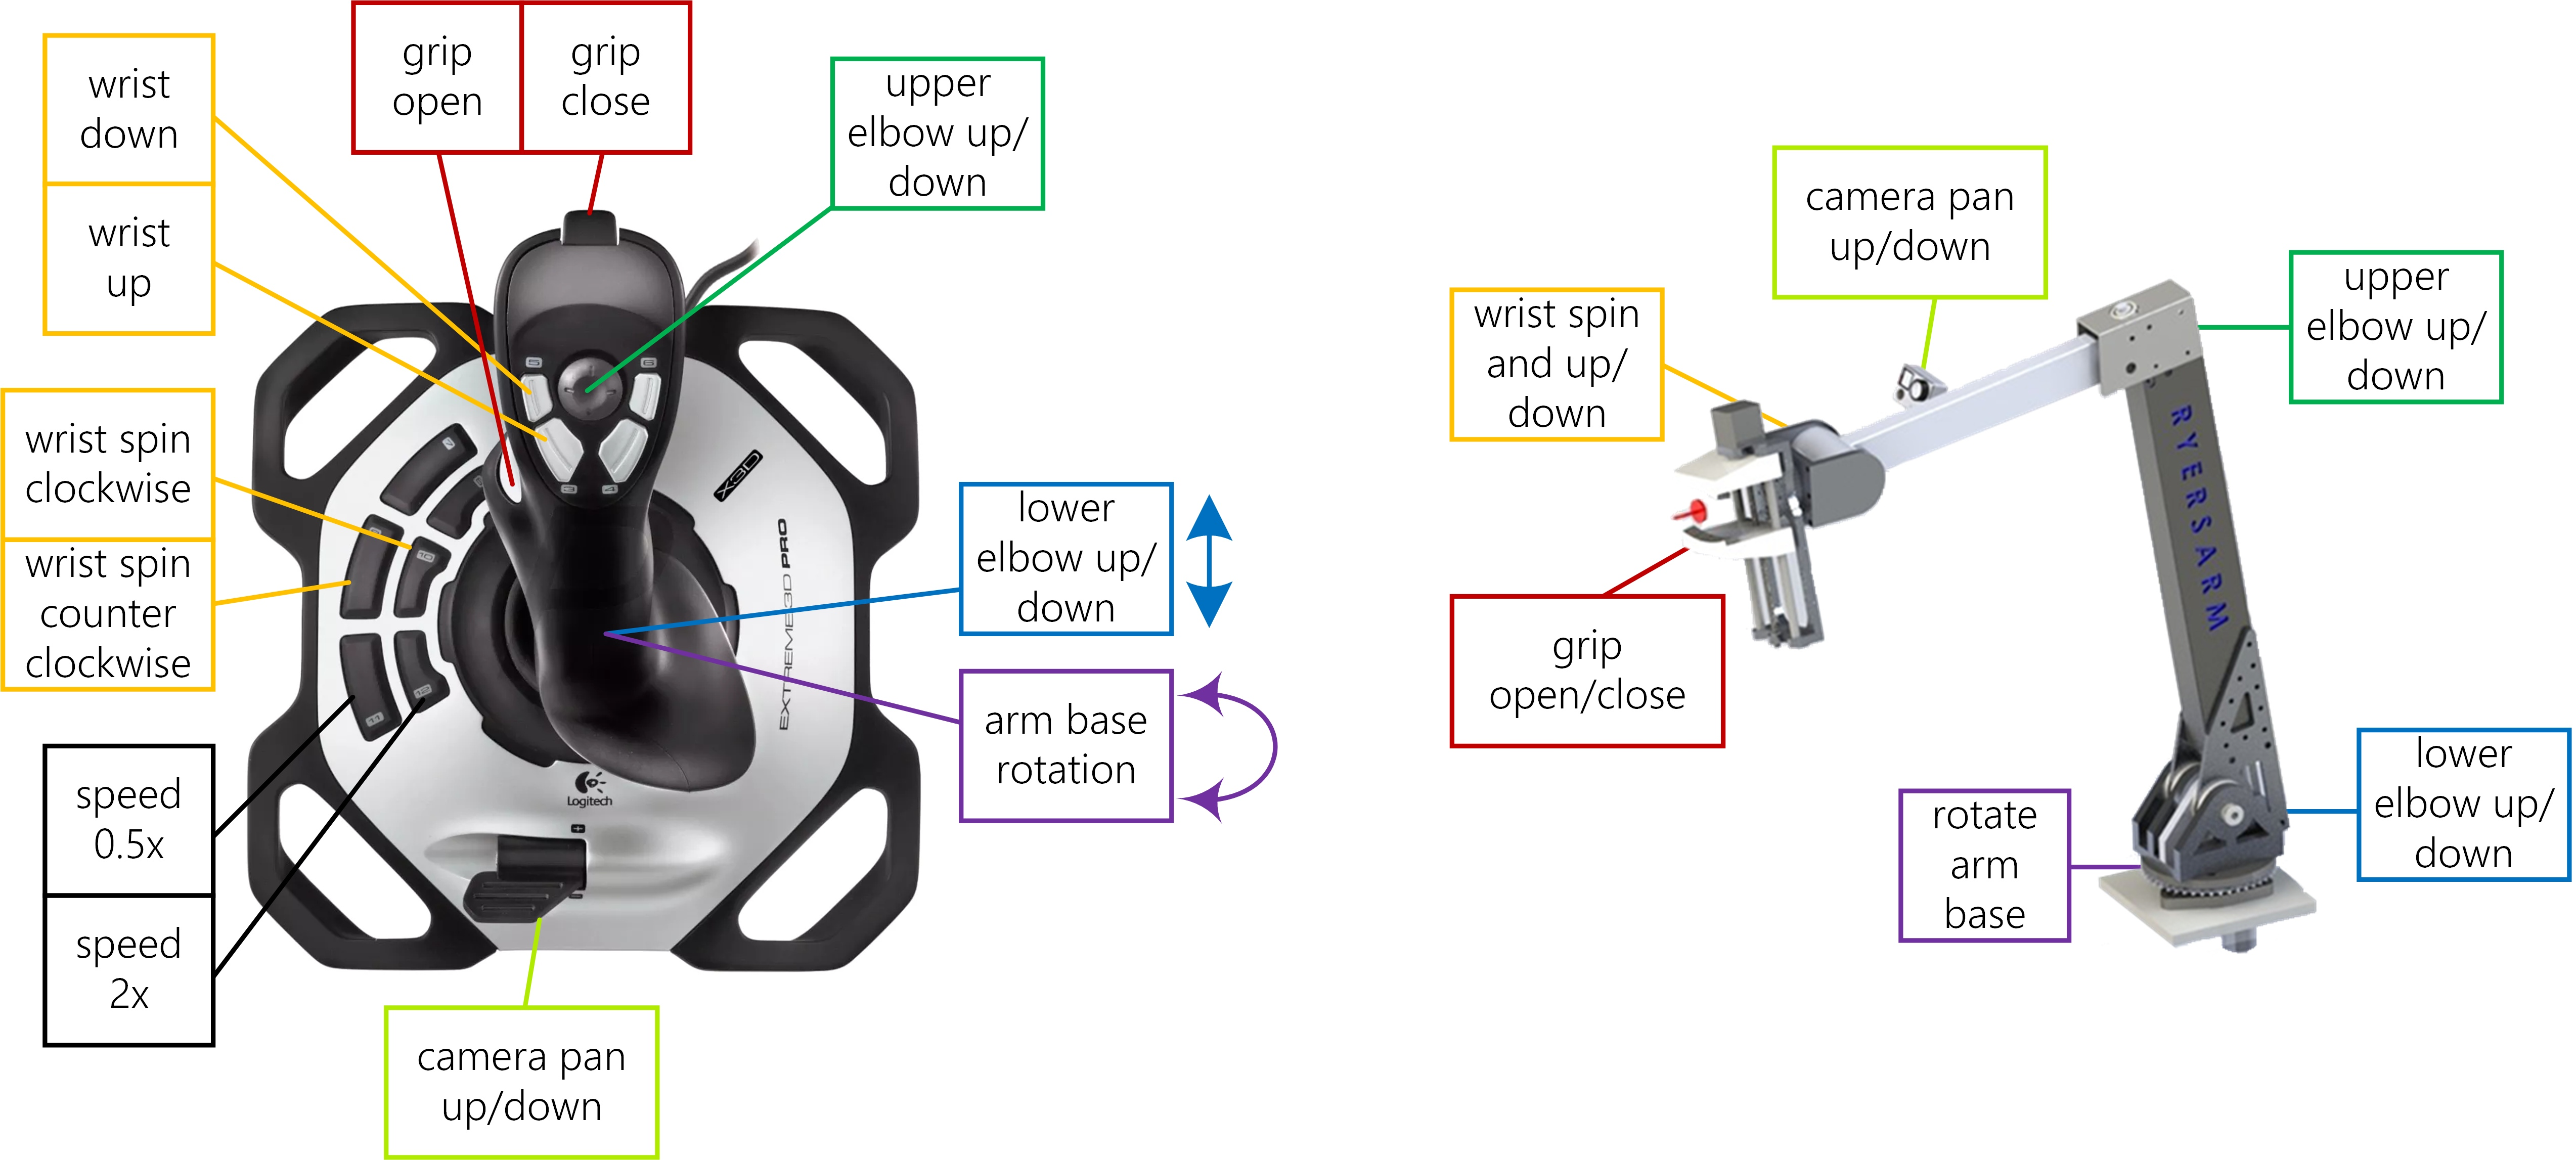
\includegraphics[width=\textwidth]{simple_arm_joystick_diagram}
\caption{The Logitech Extreme 3D Pro joystick button layout for the simple\_arm package (diagram is also available in Visio format\protect\footnotemark). Image credit: Logitech International}
\label{fig:simple_arm_joystick_diagram}
\end{figure}

\footnotetext{Logitech Extreme 3D Pro joystick button layout diagram in Visio format \url{https://github.com/danielsnider/ros-rover/blob/master/diagrams/simple_arm_joystick_diagram.vsdx?raw=true}}

Features of the simple\_arm package include: velocity control of individual arm joint motors, fast and slow motor speed modifier buttons, buttons to open and close a gripper, control of a camera servo (one axis only), simple Arduino firmware to talk to PWM motors and a servo. For the sake of simplicity, this package does not implement the following best practices: no tf publishing, no URDF, no PID control loop, no integration with ros\_control or MoveIt!. The simple\_arm package gives ROS users the ability advance their robot more quickly and hopefully to find more time to implement best practices.

\subsection{Usage Instructions}

1. Install the ROS package:

\begin{lstlisting}[frame=single,basicstyle=\ttfamily\footnotesize]
$ sudo apt-get install ros-kinetic-simple-arm
\end{lstlisting}

\noindent 2. Launch the ROS node and specify as arguments the joystick device path for controlling the arm and the Arduino to control the arm motors:

\begin{lstlisting}[frame=single,basicstyle=\ttfamily\footnotesize]
$ roslaunch simple_arm simple_arm.launch joystick_serial_dev:=/dev/input/js0 microcontroller_serial_dev:=/dev/ttyACM0
\end{lstlisting}

In most cases however, the joystick is connected to another computer, such as a teleoperation station. To do this, run the \texttt{joy} ROS node separately over the ROS network.

\noindent 3. Install the arm\_firmware onto a microcontroller as described in section \ref{drive_firmware}. The microcontroller must be connected to the arm's motors and to the on board computer running the simple\_arm ROS node by a serial connection (ex. USB).

\noindent 4. Your robot arm is ready to be moved.

\subsection{simple\_arm ROS Node}

The simple\_arm node is written in python and simply converts ROS sensor\_msgs/Joy messages from the common \texttt{joy} joystick ROS node into serial messages. The serial messages are sent to the arm\_firmware on the microcontroller to drive the robot arm. The serial messages follow a simple protocol. Each command is a list of 7 floats, one velocity command for each of the 6 joints and one target angle to control the single axis camera.

The button mapping implemented by the simple\_arm node can be seen in Fig. \ref{fig:simple_arm_joystick_diagram} and was tested on a Logitech Extreme 3D Pro joystick. The button layout should only need small modifications if any to work for similar controllers that support a DirectInput mode.

\subsection{arm\_firmware Arduino Software}\label{arm_firmware}

The arm\_firmware microcontroller code does the minimum amount of work possible to receive motor commands from a USB serial connection and output voltages to digital PWM to be received by motor controllers. It simply receives and fires commands to the lower hardware level with no feedback.

We connected an Arduino by USB serial to our robot's on-board computer and dedicated its use to the simple\_arm package. We tested on an Arduino Mega 2560, however many other boards should work with the same code and setup steps thanks to PlatformIO. You may need to change to change the pin numbers. For details on how to install and use PlatformIO with the simple\_arm package see the ROS wiki page or section \ref{drive_firmware} which contains very similar instructions.

Please note that this software does not stop moving the robot if no messages are received for certain period of time. 

\section{Tutorial: Autonomous Recovery after Lost Communications}\label{lostcomms}
At the URC competition, Team R3 (Ryerson University) was worried about travelling into a communication deadzone and losing wireless control of our rover from a distant base station. This is one of the challenges put forth by URC competition and is often found in the real world.

We have published a new package, called lost\_comms\_recovery\footnote{Source code for lost\_comms\_recovery ROS package \url{https://github.com/danielsnider/lost_comms_recovery}}\footnote{Wiki page for lost\_comms\_recovery ROS package \url{http://wiki.ros.org/lost_comms_recovery}} that will trigger when the robot loses connection to the base station and it will navigate to a configurable home or stop all motors. The base station connection check uses ping to a configurable list of IPs. The monitoring loop waits 3 seconds between checks and by default failure is triggered after 2 consecutive failed pings. Each ping will wait up to one second to receive a response. 

Please note that this node is not designed to be $realtime$\footnote{More information about real-time computing \url{https://en.wikipedia.org/wiki/Real-time_computing}} safe. What is safer than relying on this package is using motor control software that sets zero velocity after a certain amount of time not receiving any new commands.

\subsection{Usage Instructions}

1. Install:

\begin{lstlisting}[frame=single,basicstyle=\ttfamily\footnotesize,breaklines=true]
$ sudo apt-get install ros-kinetic-lost-comms-recovery
\end{lstlisting}

\noindent 2. Launch:

\begin{lstlisting}[frame=single,basicstyle=\ttfamily\footnotesize,breaklines=true]
$ roslaunch lost_comms_recovery lost_comms_recovery.launch ips_to_monitor:=192.168.1.2
\end{lstlisting}

\noindent 3. Then the following behavior will take place:

\subsubsection*{If move\_base is running,} an autonomous recovery navigation will take place. The default position of the recovery goal is the origin (0,0) of the frame given it the goal\_frame\_id ROS parameter and the orientation is all 0s by default. This default pose can be overridden if a messaged is published on the recovery\_pose topic. If move\_base is already navigating to a goal it will not be interrupted and recovery navigation will happen when move\_base is idle.

\subsubsection*{If move\_base is not running} when communication failure occurs then motors and joysticks are set to zero by publishing a zero geometry\_msgs/Twist message and a zero sensor\_msgs/Joy message to simulate a joystick returning to a neutral, non-active position.

\subsection{Normal Output}

When you launch and use the lost\_comms\_recovery ROS node you will see the following console output.

\begin{lstlisting}[frame=single,basicstyle=\ttfamily\footnotesize,breaklines=true]
$ roslaunch lost_comms_recovery lost_comms_recovery.launch ips_to_monitor:=192.168.190.136

[INFO] Monitoring base station on IP(s): 192.168.190.136.
[INFO] Connected to base station.
[INFO] Connected to base station.
...
[ERROR] No connection to base station.
[INFO] Executing move_base goal to position (x,y) 0.0, 0.0.
[INFO] Initial goal status: PENDING
[INFO] This goal has been accepted by the simple action server
[INFO] Final goal status: SUCCEEDED
[INFO] Goal reached.
\end{lstlisting}



\section{Tutorial: Stitch Panoramas with Hugin}\label{pano}

Hugin\cite{hugin} is professional software popularly used to create panoramic images by compositing and rectifying multiple still images. We have created a package called hugin\_panorama\footnote{Source code for hugin\_panorama ROS package \url{https://github.com/danielsnider/hugin_panorama}}\footnote{Wiki page for hugin\_panorama ROS package \url{http://wiki.ros.org/hugin_panorama}} to wrap one high level function of Hugin, the creation of panoramas. 

In the science task of the URC competition, teams are awarded points if they document locations of scientific interest such as geological and soil sampling sites with panoramas.

Our package uses the Hugin command line tools\footnote{The Hugin image processing library \url{http://hugin.sourceforge.net/}} to compose panoramas in 8 steps according to a well-documented workflow\footnote{Panorama scripting with Hugin \url{http://wiki.panotools.org/Panorama_scripting_in_a_nutshell}}. To summarize, it consists of creating a Hugin project file, finding matching feature control points between images, pruning control points with large error distances, find vertical lines across images to be straighten, doing the straightening and other photometric optimization, optimal cropping, and saving to tiff and compressed png image formats. The compressed panoramic image is published on at output ROS topic. An example panorama can be seen in Fig. \ref{fig:pano}.

The hugin\_panorama launch implementation\footnote{Main launch file of the hugin\_panorama package \url{https://github.com/danielsnider/hugin_panorama/blob/master/launch/hugin_panorama.launch}} makes use of the image\_saver\footnote{Documentation for the image\_saver ROS node \url{http://wiki.ros.org/image_view#image_view.2BAC8-diamondback.image_saver}} node provided by the image\_view package. The image\_saver node will save all images from a sensor\_msgs/Image topic as jpg/png files. The saved images are used as the source image parts when creating the panoramas.
 
\begin{figure}
\centering
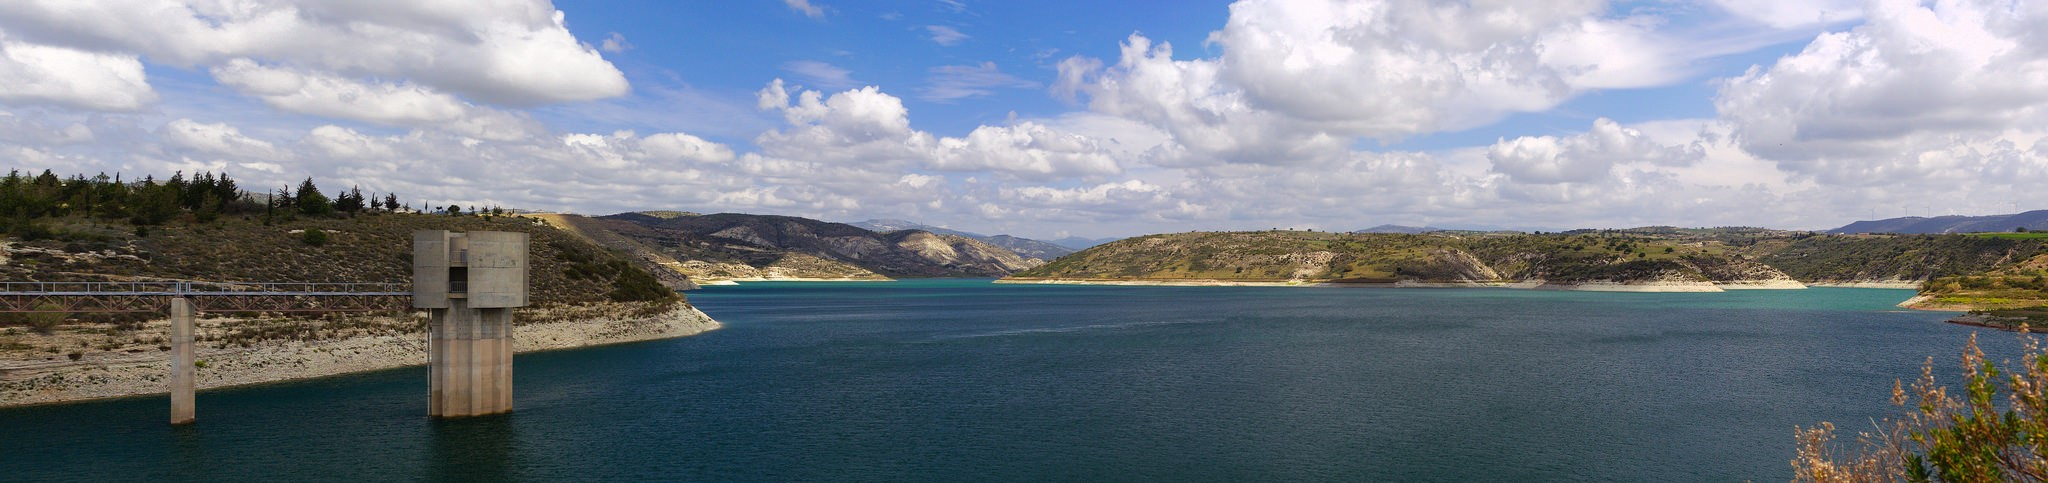
\includegraphics[width=\textwidth]{pano}
\caption{Panorama example made with Hugin. Image credit: Senza Senso}
\label{fig:pano}
\end{figure}  

\subsection{Usage Instructions}

1. Install the ROS package:

\begin{lstlisting}[frame=single,basicstyle=\ttfamily\footnotesize,breaklines=true]
$ sudo apt-get install ros-kinetic-hugin-panorama hugin-tools enblend
\end{lstlisting}

\noindent 2. Launch the ROS node:

\begin{lstlisting}[frame=single,basicstyle=\ttfamily\footnotesize,breaklines=true]
$ roslaunch hugin_panorama hugin_panorama.launch image:=/image_topic
\end{lstlisting}

\noindent 3. Save individual images for input to the panorama: (order doesn't matter)

\begin{lstlisting}[frame=single,basicstyle=\ttfamily\footnotesize,breaklines=true]
$ rosservice call /hugin_panorama/image_saver/save
# change angle of camera
$ rosservice call /hugin_panorama/image_saver/save
# repeat as many times as you like...
\end{lstlisting}

\noindent 4. Stitch the panorama:

\begin{lstlisting}[frame=single,basicstyle=\ttfamily\footnotesize,breaklines=true]
$ rosservice call /hugin_panorama/stitch
\end{lstlisting}

\noindent 5. View resulting panorama:

\begin{lstlisting}[frame=single,basicstyle=\ttfamily\footnotesize,breaklines=true]
$ rqt_image_view /hugin_panorama/panorama/compressed
# or open the panorama file
$ roscd hugin_panorama; eog ./images/output.png
\end{lstlisting}

\noindent 6. Start again:

\begin{lstlisting}[frame=single,basicstyle=\ttfamily\footnotesize,breaklines=true]
$ rosservice call /hugin_panorama/reset
\end{lstlisting}

This command will clear the images waiting to be stitched so you can start collecting images for an entirely new panorama.


\subsection{Live Panorama Mode}

If you have more than one camera on your robot and you want to stitch them together repetitively in a loop, then use stitch\_loop.launch. However, expect a slow frame rate of less than 1 Hz because this package is not optimized for speed.

\noindent 1. Launch the stitch\_loop node:

\begin{lstlisting}[frame=single,basicstyle=\ttfamily\footnotesize,breaklines=true]
$ roslaunch hugin_panorama stitch_loop.launch image1:=/image_topic2 image2:=/image_topic2
\end{lstlisting}

\noindent 2. View resulting live panorama:

\begin{lstlisting}[frame=single,basicstyle=\ttfamily\footnotesize,breaklines=true]
$ rqt_image_view /hugin_panorama/panorama/compressed
\end{lstlisting}

If you have more than two cameras then the quick fix is you'll to edit the simple python script (\texttt{rosed hugin\_panorama stitch\_loop.py}) and the launch file (\texttt{rosed hugin\_panorama stitch\_loop.launch}) to duplicate some parts.


\section{Tutorial: GPS Navigation Goal}\label{gpsnav}

In the autonomous task of the URC competition, a series of goal locations are given to teams as approximate GPS coordinates. Rovers are expected to autonomously drive to the GPS location and then find and stop near a tennis ball marker. To achieve the GPS navigation requirements of this task, Team R3 has created the gps\_goal\footnote{Source code for gps\_goal ROS package \url{https://github.com/danielsnider/gps_goal}}\footnote{Wiki page for gps\_goal ROS package \url{http://wiki.ros.org/gps_goal}} package. We believe this is the first packaged for ROS solution to convert navigation goals in given in GPS coordinates to ROS frame coordinates. The package uses one known GPS location in the ROS frame to facilitate converting between coordinate systems. Fig. \ref{fig:GPS_goal_Diagram2} shows how this package fits into Team R3's larger ROS software architecture.

\begin{figure}
\centering
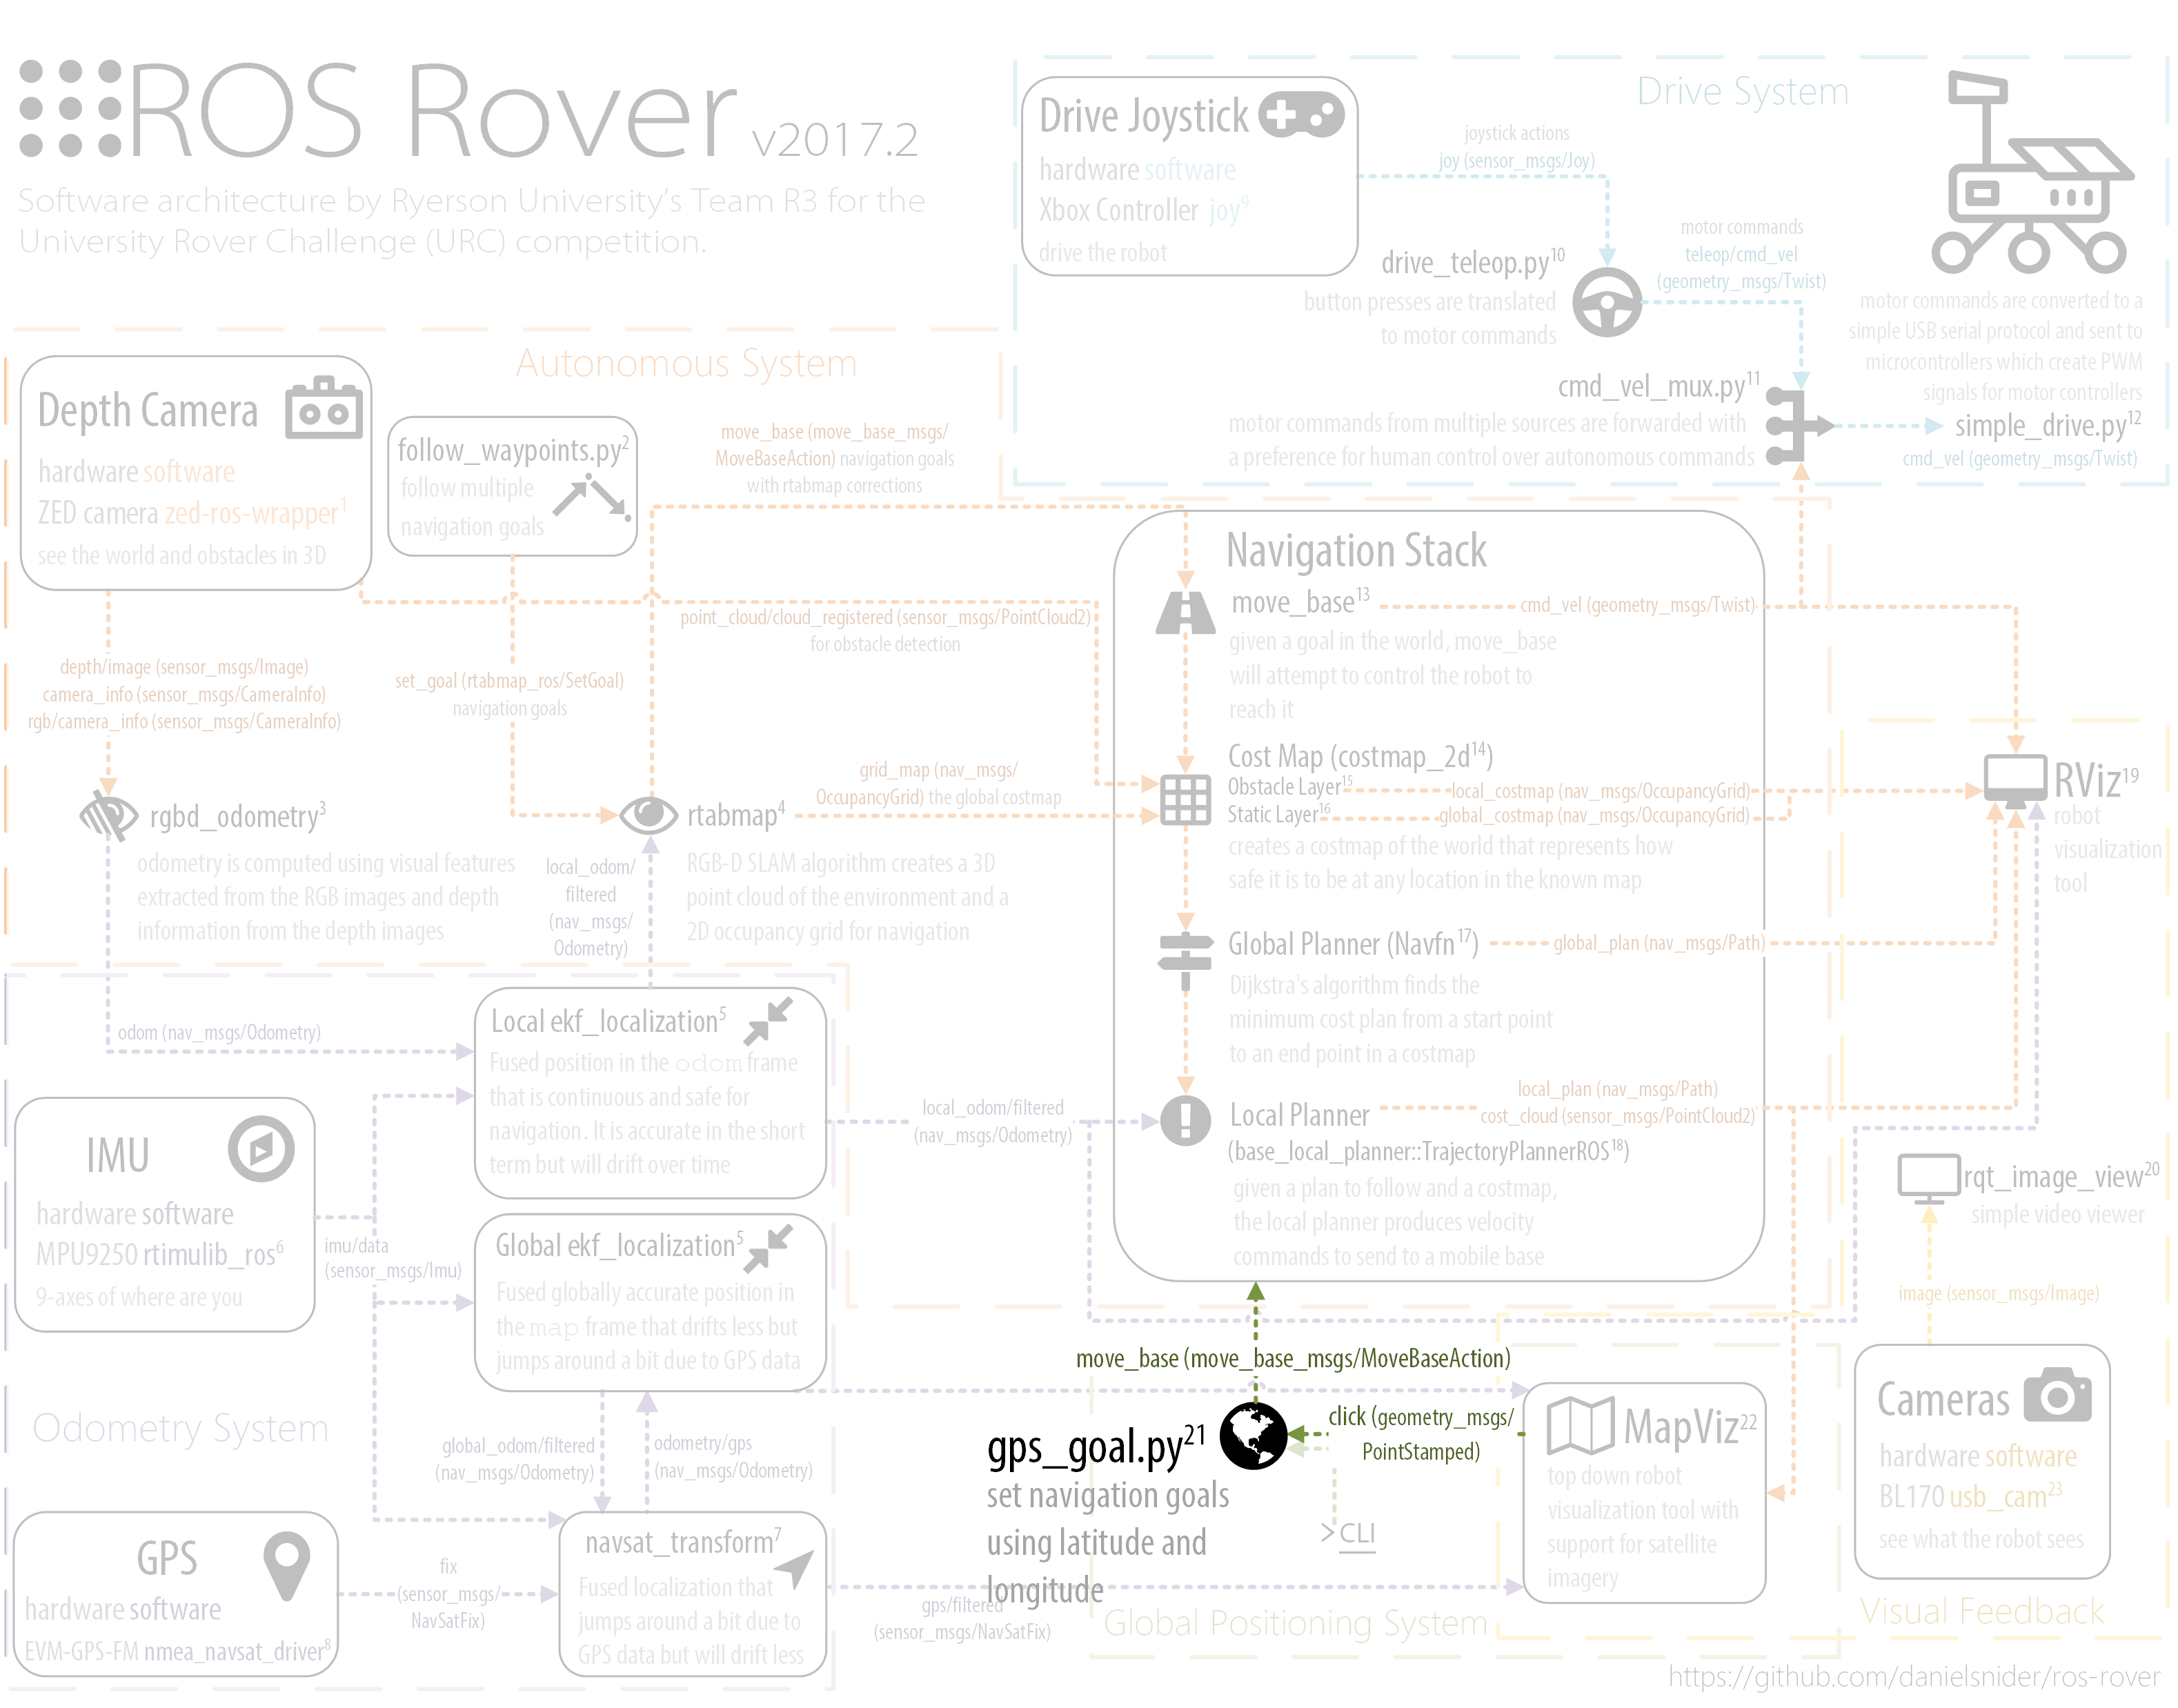
\includegraphics[width=\textwidth]{GPS_goal_Diagram2}
\caption{The gps\_goal ROS node seen within Team R3's rover system. See fig. \ref{fig:Diagram} for the full diagram.}
\label{fig:GPS_goal_Diagram2}
\end{figure}


The new gps\_goal package uses the WGS84 ellipsoid\footnote{The World Geodetic System (WGS) 84 is the reference coordinate system used by the Global Positioning System (GPS). WGS84 uses degrees. It consists a latitudinal axis from -90 to 90 degrees and a longitudinal axis from -180 to 180 degrees. As it is the standard coordinate system for GPS it is also commonly used in robotics. \url{https://en.wikipedia.org/wiki/World_Geodetic_System#A_new_World_Geodetic_System:_WGS_84}} and geographiclib\footnote{The GreographicLib software library \url{https://geographiclib.sourceforge.io/}} python library to calculate the surface distance between GPS points. WGS84 is the standard coordinate system for GPS and thus the packages configures GreographicLib to use it because it is important for calculating the correct distance between GPS points.

The GPS goal can be set using a geometry\_msgs/PoseStamped or sensor\_msgs/NavSatFix message. The robot's desired yaw, pitch, and roll can be set in a PoseStamped message but when using a NavSatFix they will always be set to 0 degrees.

The goal is calculated in a ROS coordinate frame by comparing the goal GPS location to a known GPS location at the origin (0,0) of a ROS frame given by the local\_xy\_frame ROS parameter which is typically set to 'world' but can be any ROS frame. This initial origin GPS location is best published using a helper initialize\_origin node (see section \ref{init_origin} below for more details).

\subsection{Usage Instructions}

1. Install the ROS package:

\begin{lstlisting}[frame=single,basicstyle=\ttfamily\footnotesize,breaklines=true]
$ sudo apt-get install ros-kinetic-gps-goal
\end{lstlisting}

\noindent 2. Launch the ROS node:

\begin{lstlisting}[frame=single,basicstyle=\ttfamily\footnotesize,breaklines=true]
$ roslaunch gps_goal gps_goal.launch
\end{lstlisting}


\noindent 3. Set a known GPS location using one of the following approaches (a) or (b). The given GPS location will be attached to the origin (0,0) of the ROS frame given by the local\_xy\_frame ROS parameter. This is used to calculate the distance to the goal.

3a. Use the next GPS coordinate published on a ROS topic (requires package ros-kinetic-swri-transform-util):

\begin{lstlisting}[frame=single,basicstyle=\ttfamily\footnotesize,breaklines=true]
$ roslaunch gps_goal initialize_origin.launch origin:=auto
\end{lstlisting}

3b. Or set the initial origin manually using a rostopic publish command:
\begin{lstlisting}[frame=single,basicstyle=\ttfamily\footnotesize,breaklines=true]
$ rostopic pub /local_xy_origin geometry_msgs/PoseStamped '{ header: { frame_id: "/map" }, pose: { position: { x: 43.658, y: -79.379 } } }' -1
\end{lstlisting}

\noindent 4. Set a navigation goal using GPS coordinates set with either a Pose or NavSatFix GPS message.

\begin{lstlisting}[frame=single,basicstyle=\ttfamily\footnotesize,breaklines=true]
$ rostopic pub /gps_goal_fix sensor_msgs/NavSatFix "{latitude: 38.42, longitude: -110.79}" -1
OR
$ rostopic pub /gps_goal_pose geometry_msgs/PoseStamped '{ header: { frame_id: "/map" }, pose: { position: { x: 43.658, y: -79.379 } } }' -1
\end{lstlisting}


\subsection{Command Line Interface (CLI)}

Alternatively, a Command Line Interface (CLI) is available to set GPS navigation goals. When using the CLI interface you can use one of two coordinate formats: either degree, minute, and seconds (DMS) or decimal GPS format. Using command line arguments, users can also set the desired roll, pitch, and yaw final position. You can invoke the gps\_goal script once using the Command Line Interface (CLI) with any of the following options.

\begin{lstlisting}[frame=single,basicstyle=\ttfamily\footnotesize,breaklines=true,caption={Example usages of the gps\_goal CLI script to set a navigation goal.}]
$ roscd gps_goal
$ ./src/gps_goal/gps_goal.py --lat 43.658 --long -79.379 # decimal format
OR 
$ ./src/gps_goal/gps_goal.py --lat 43,39,31 --long -79,22,45 # DMS format
\end{lstlisting}

\subsection{initialize\_origin Helper ROS Node}\label{init_origin}
The initialize\_origin node will continuously publish (actually in a latched\footnote{When a connection is latched, the last message published is saved and automatically sent to any future subscribers of that connection.} manner) a geometry\_msgs/PoseStamped on the local\_xy\_origin topic and this is the recommended approach over  manually publishing the origin GPS location with rostopic pub. This location is the origin (0,0) of the frame (typically world) given by the local\_xy\_frame parameter to the initialize\_origin node. This location is used to calculate distances for goals. One message on this topic is consumed when the node starts only.

This node is provided by the swri\_transform\_util package (apt-get install ros-kinetic-swri-transform-util) and it is often launched as a helper node for MapViz, a top-down robot and world visualization tool that is detailed in section \ref{mapviz}. There are two modes for initialize\_origin: static or auto.

\subsubsection*{Static Mode}
You can hard code a GPS location (useful for testing) for the origin (0,0). In the following example the coordinates for the Mars Desert Research Station (MDRS) are hard coded in initialize\_origin.launch and selected on the command line with the option "origin:=MDRS".
\begin{lstlisting}[frame=single,basicstyle=\ttfamily\footnotesize,breaklines=true]
$ roslaunch gps_goal initialize_origin.launch origin:=MDRS
\end{lstlisting}

\subsubsection*{Auto Mode}
When using the "auto" mode, the origin will be to the first GPS fix that it receives on the topic configured in the initialize\_origin.launch file.
\begin{lstlisting}[frame=single,basicstyle=\ttfamily\footnotesize,breaklines=true]
$ roslaunch gps_goal initialize_origin.launch origin:=auto
\end{lstlisting}

\subsubsection*{Launch example}
Starting the initialize\_origin ROS node can be done in the following way.

\begin{lstlisting}[frame=single,basicstyle=\ttfamily\footnotesize,breaklines=true,caption={An example launch config to start the initialize\_origin ROS node.}]
<node pkg="swri_transform_util" type="initialize_origin.py" name="initialize_origin" output="screen">
  <param name="local_xy_frame" value="/world"/>
  <param name="local_xy_origin" value="MDRS"/> <!-- setting "auto" here will set the origin to the first GPS fix that it receives -->
  <remap from="gps" to="gps"/>
  <rosparam param="local_xy_origins">
    [{ name: MDRS,
       latitude: 38.40630,
       longitude: -110.79201,
       altitude: 0.0,
       heading: 0.0}]
  </rosparam>
</node>
\end{lstlisting}

\subsection{Normal Output}
When you launch and use the gps\_goal ROS node or CLI interface you will see the following console output.

\begin{lstlisting}[frame=single,basicstyle=\ttfamily\footnotesize,breaklines=true]
$ roscd gps_goal
$ ./src/gps_goal/gps_goal.py --lat 43.658 --long -79.379

[INFO]: Connecting to move_base...
[INFO]: Connected.
[INFO]: Waiting for a message to initialize the origin GPS location...
[INFO]: Received origin: lat 43.642, long -79.380.
[INFO]: Given GPS goal: lat 43.658, long -79.379.
[INFO]: The distance from the origin to the goal is 97.3 m.
[INFO]: The azimuth from the origin to the goal is 169.513 degrees.
[INFO]: The translation from the origin to the goal is (x,y) 91.3, 13.6 m.
[INFO]: Executing move_base goal to position (x,y) 91.3, 13.6, with 138.14 degrees yaw.
[INFO]: To cancel the goal: 'rostopic pub -1 /move_base/cancel actionlib_msgs/GoalID -- {}'
[INFO]: Inital goal status: PENDING
[INFO]: Final goal status: COMPLETE
\end{lstlisting}



\section{Tutorial: Wireless Communication}\label{wireless}

At Team ITU (Istanbul Technical University), communication from our base station to our mobile outdoor rover was of utmost importance and received a good amount of development time. Non-line of sight (NLOS) communication is an important issue and often a cause of unsuccessful runs in URC. Although there are various commercial products available claiming to solve the issues of long range and high throughput communication, many of them don't solve the problems as advertised. So a combination of systems and products were tested and used in the competition\footnote{Team ITU's low level communication source code \url{https://github.com/itu-rover/2016-2017-Sensor-GPS-STM-Codes-/blob/master/STM32/project/mpu_test/Src/main.c}}\footnote{Team ITU's high level communication source code \url{https://github.com/itu-rover/communication}}.

The primary system must be capable of delivering a video feed to the ground station for operators to use while piloting the vehicle remotely. This system is generally preferred to be a Wi-Fi network that can multiplex high-res video and data traffic at high speeds. After performing a series of unsuccessful non-line of sight (NLOS) tests at long distances (400-500 meters) with the Ubiquiti Bullet M2, a popular 2.4 GHz product, a less popular Microhard pDDL2450 module was chosen based on our sponsor's advice. Thankfully, the sponsor had a few spares and donated them to Team ITU. In tests, this 2.4 GHz module was generally successful in sending useful data from the vehicle's instruments and 720p video feed compressed with MJPEG from five cameras at the same time over a 1 km range in NLOS course with 8dBi omnidirectional antennas. This module is physically connected to the high level on-board computer (OBC), a Raspberry Pi 3 with running Ubuntu 16.04, with a standard CAT5 Ethernet cable.

Secondly, our radio frequency (RF) backup link was able to pass over the natural obstacles such as large rocks and hills. This link operates on lower UHF frequencies and lower baud rates to increase performance needed to send crucial information about the vehicle's condition to ensure health and function of the rover at extreme distances (5km). We consider our rover's heartbeat, GPS position, attitude and current speed to be important data that should be sent through the RF link. Tests were conducted using 433Mhz LoRa modules (see Fig. \ref{fig:lora}) on both sides with 3dBi omnidirectional antennas, in 9600 and 115200 baud rates. The tests showed that these modules have no problem sending the data over a 5 km range in NLOS conditions. The LoRa modules were wired to the standard RX-TX wires on our STM32F103 microprocessor and uses UART communication. The microprocessor also controls the driving system, communicates with the sensors, the Raspberry Pi 3 on-board computer (OBC). 

% \pagebreak[4]

\begin{figure}
\centering
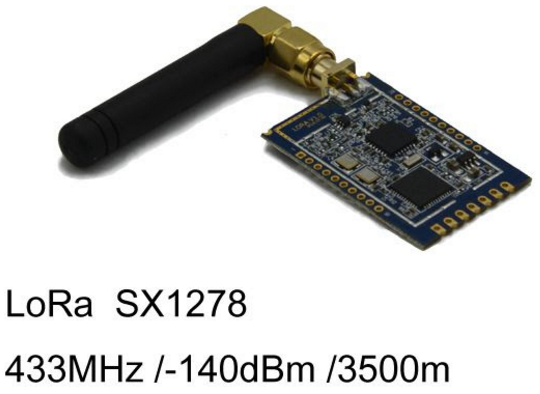
\includegraphics[height=3.5cm]{lora}
\caption{UHF LoRa radio module for long range communication. Image credit: Semtech Corporation}
\label{fig:lora}
\end{figure}

To make the LoRa RF link active in the C\# language see Listing \ref{lst:lora}.

\begin{lstlisting}[frame=single,basicstyle=\ttfamily\footnotesize,breaklines=true,label={lst:lora},caption={Start communication with the LoRa RF module in the C\# language.}]
 SerialPort _serialPort = new SerialPort("COM1", 115200, Parity.None, 8, StopBits.One);
_serialPort.Open();
\end{lstlisting}

In normal, connected conditions, only the Wi-Fi network system is active and the RF system is inactive. In these conditions all the processing is done in the Raspberry Pi 3 on-board computer (OBC). Commands from the human pilot reach the OBC first and then are distributed to the low level STM microprocessor via a RS232 link. The video feed is active and the pilot can easily drive the rover using the video images from the cameras. The low band RF system was remarkably reliable although interruptions were encountered at times with the Wi-Fi network. 

\begin{figure}[H]
\centering
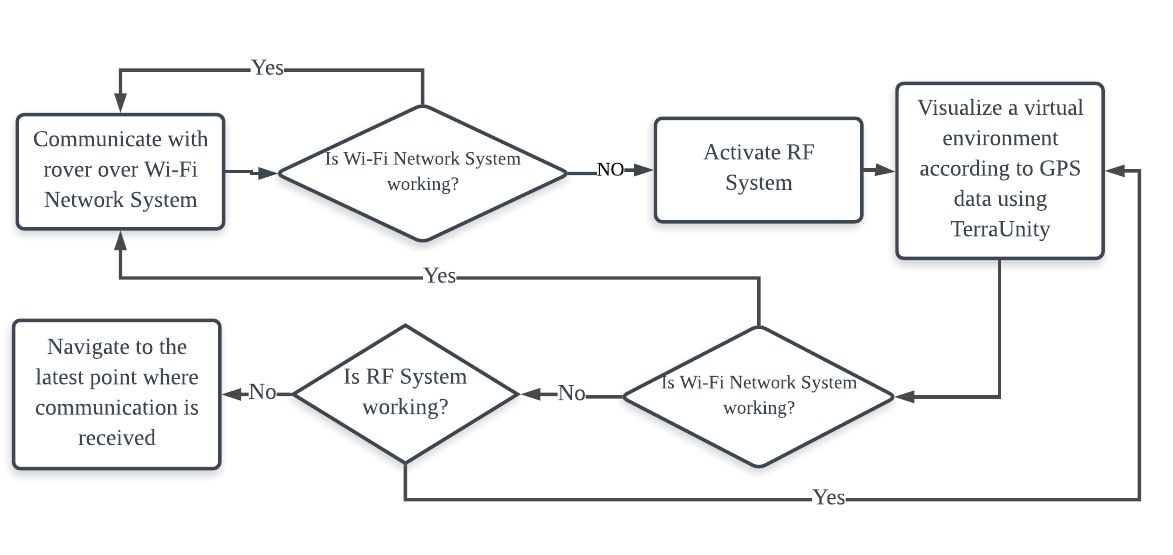
\includegraphics[width=\textwidth]{comms}
\caption{Flowchart of decision making algorithm used on ITU's rover.}
\label{fig:comms}
\end{figure}

In the case of losing the Wi-Fi network system or OBC, the video feed will be lost and piloting the vehicle without a video feed is almost impossible. So an innovative solution was implemented to overcome this problem and continue the mission. In such condition, first the RF link is activated and crucial information and the pilot commands are redirected to this link. Therefore, the pilot directly communicates with low level processor. To help the pilot visualize the environment a virtual environment around the GPS coordinates is simulated with computer graphics. This visual environment is created using the TerraUnity software. The software creates a one-to-one, colorized, topographical landscape with natural objects loaded from a 3D map database of the location\footnote{TerraUnity computer graphics software used to the visualize the rover at its GPS location in a topographical simulation of earth \url{http://terraunity.com/}}. This way the driver could look at the ground station monitor and see the terrain around the vehicle in the Unity graphics simulation, which was pretty precise in our tests. The software was found to be very successful in creating a realistic environment and it gives a clue to the driver about where the vehicle is and what natural obstacles are around it. Knowing the locations of natural obstacles is essential as the rover has physical limits that prevents it from navigating some terrain. Although the TerraUnity solution is an imperfect representation of the world, it provides a useful avenue to continue the mission in a catastrophic failure scenario.

Finally, in the case where both Wi-Fi and RF communication is lost to the rover, a third backup system is initialized where the rover navigates autonomously to the last GPS point that it communicated successfully with the ground station.

\section{Tutorial: Autonomous Navigation by Team R3}\label{r3auto}

In this section we present Team R3's (Ryerson University) autonomous software architecture that was designed for outdoor autonomous driving at the University Rover Competition (URC) 2017. The design uses a stereo camera and SLAM to navigate to a goal autonomously and avoid static obstacles. For a description of the requirements of the autonomous task for URC 2017, please refer back to Section \ref{urcrules} of this chapter.

In the following subsections we will elaborate on the ZED stereo camera, rbgd\_odometry, RTAB-Map SLAM, and move\_base. Fig. \ref{fig:r3auto} depicts a diagram of Team R3's autonomous software design. To see this diagram within a larger diagram with more of Team R3's rover software components see Section \ref{r3case}.


\begin{sidewaysfigure}
\centering
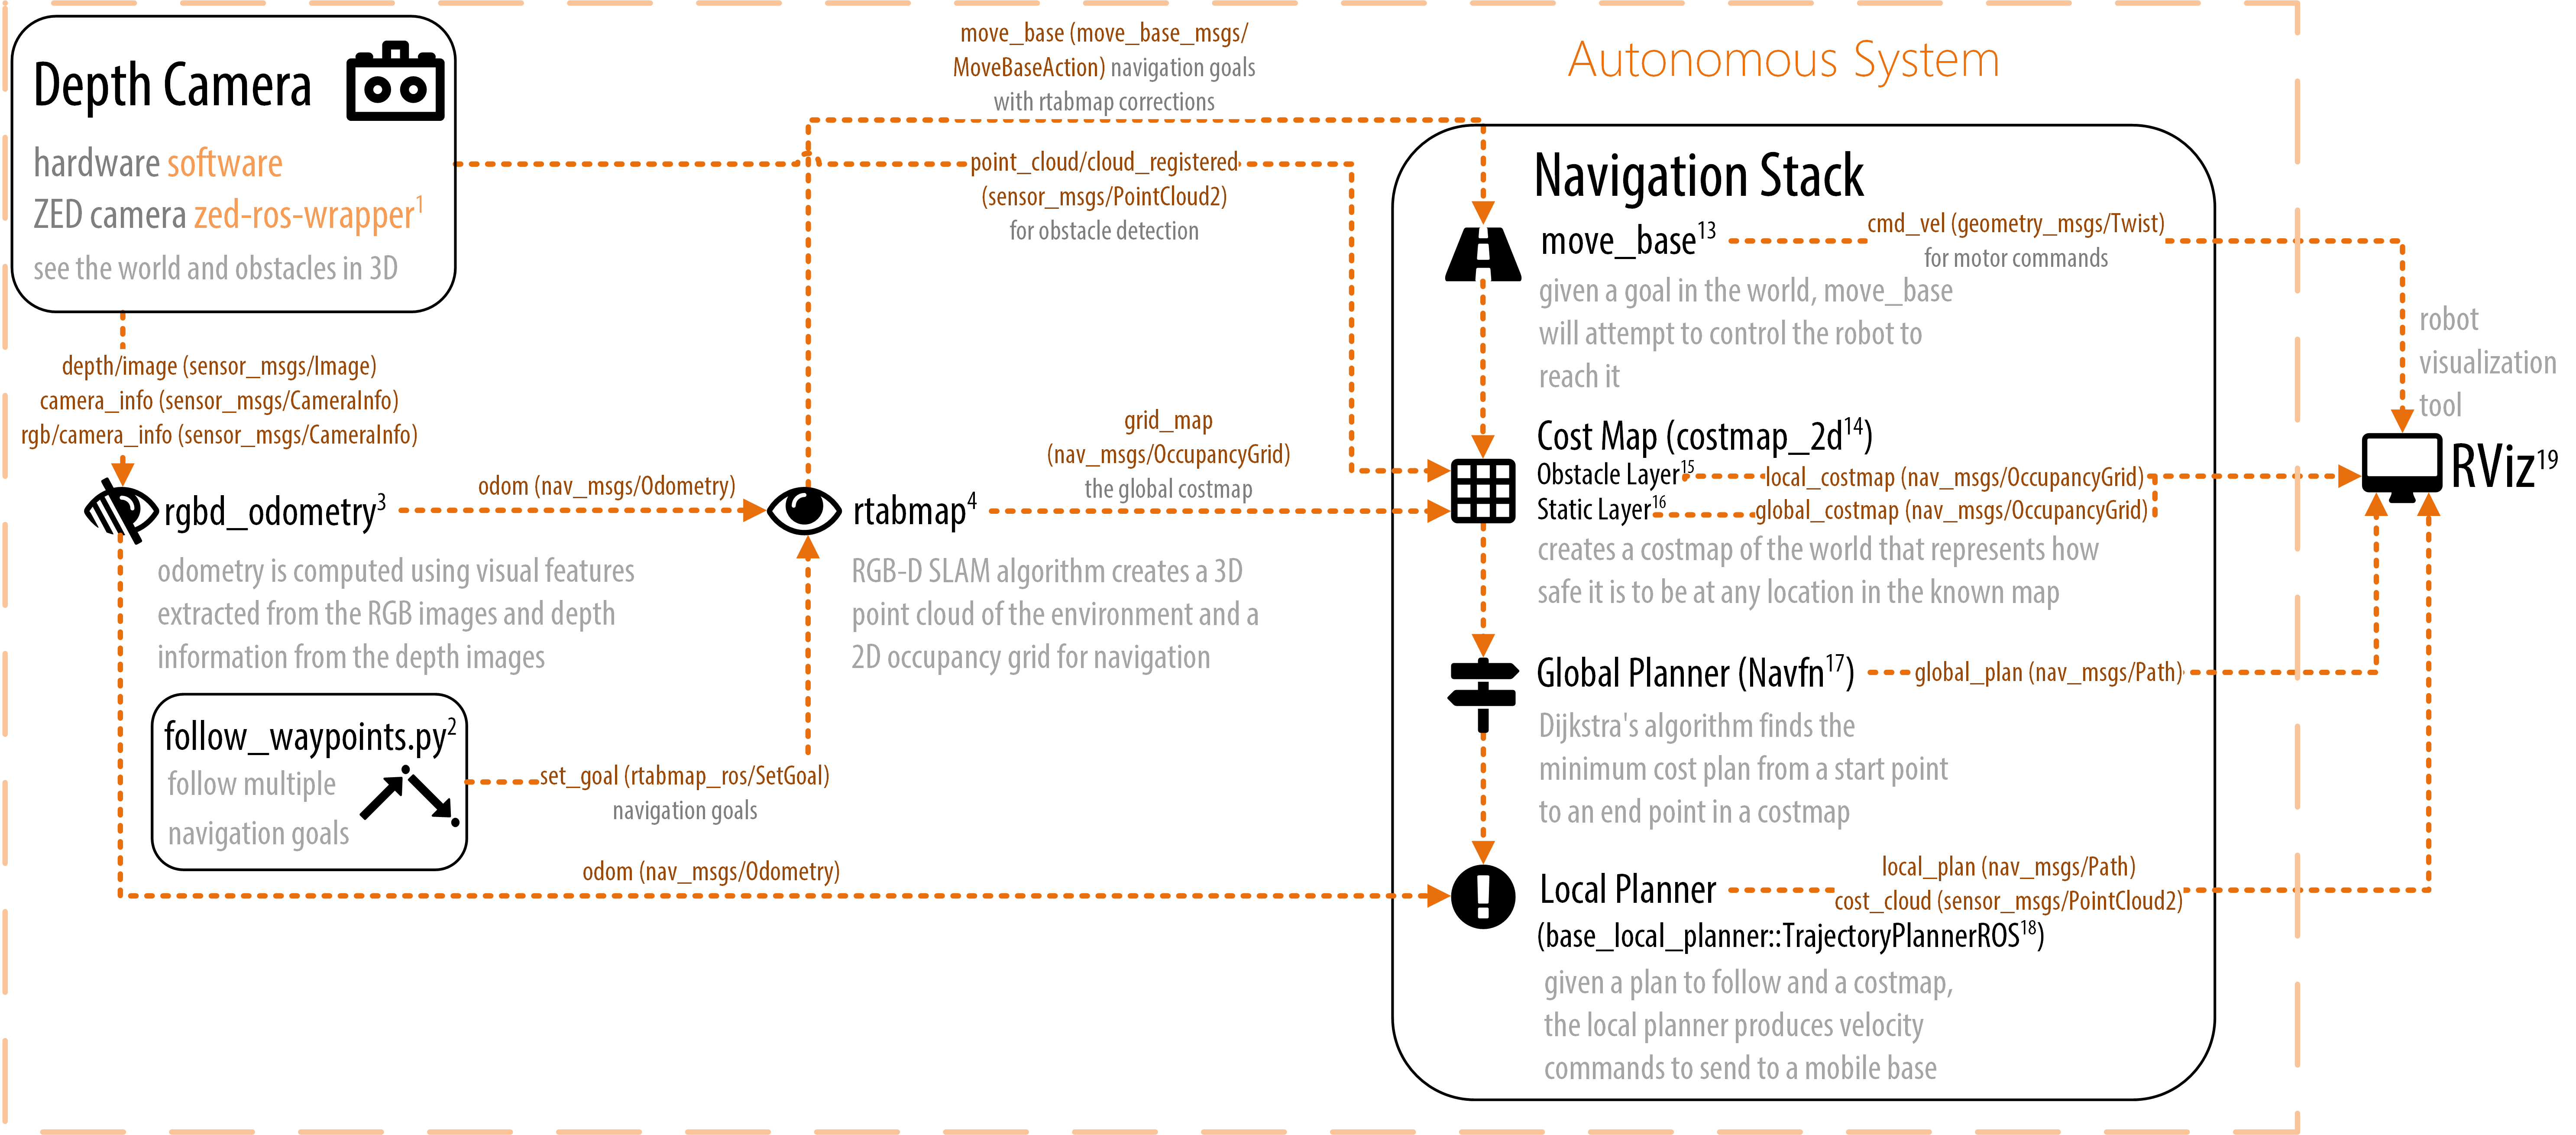
\includegraphics[width=\textwidth]{r3auto}
\caption{Team R3's autonomous navigation system used at URC 2017 rover competition. This diagram is also available in Visio format\protect\footnotemark.}
\label{fig:r3auto}
\end{sidewaysfigure}

\footnotetext{Team R3's autonomous software architecture diagram in Microsoft Visio format \url{https://github.com/danielsnider/ros-rover/blob/master/diagrams/team_r3_AUTO_Diagram.vsdx?raw=true}}



% \begin{figure}
% \centering
% 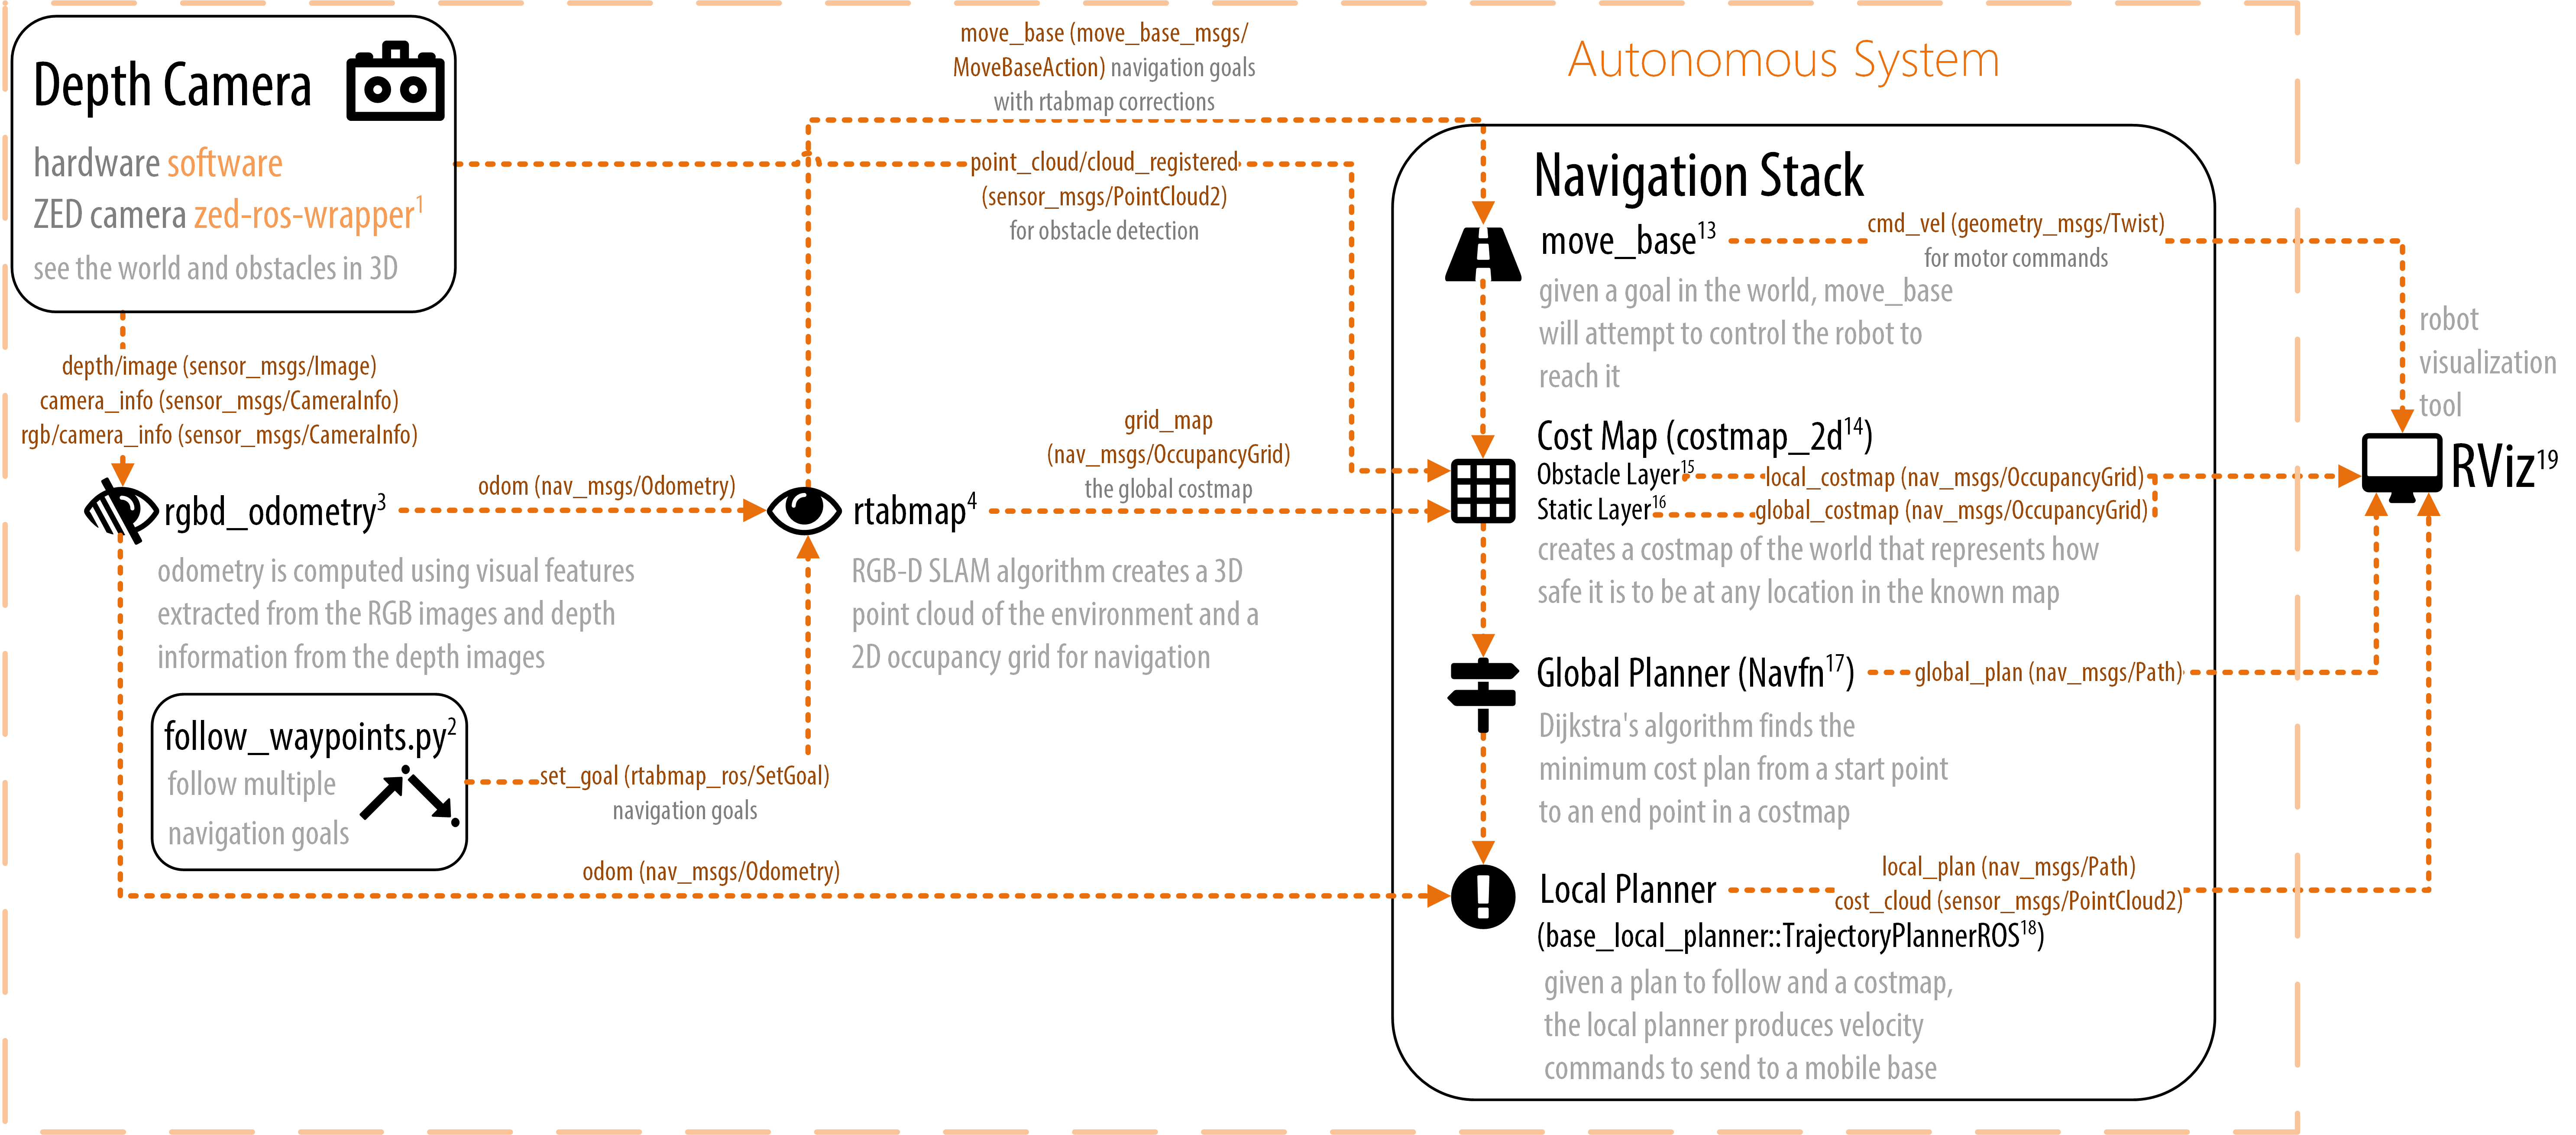
\includegraphics[width=\textwidth]{r3auto}
% \caption{Team R3's autonomous navigation system used at URC 2017 rover competition. This diagram is also available in Visio format.}
% \label{fig:r3auto}
% \end{figure}

\subsection{ZED Depth Camera}\label{sec:zed}

\begin{figure}
\centering
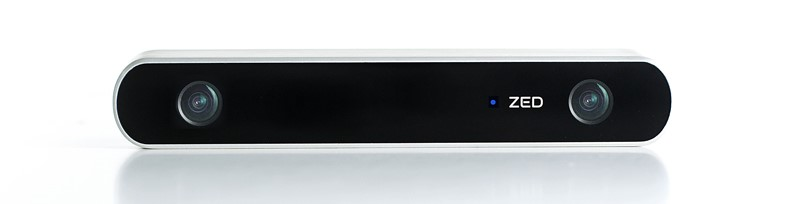
\includegraphics[width=\textwidth]{zed}
\caption{The ZED depth camera. Image credit: Stereolabs}
\label{fig:zed}
\end{figure}

The ZED stereo camera\footnote{ZED stereo camera technical specs \url{https://www.stereolabs.com/zed/}}\footnote{More ZED camera documentation \url{https://www.stereolabs.com/documentation/guides/using-zed-with-ros/ZED_node.html}}\footnote{Team R3's ZED launch file \url{https://github.com/teamr3/URC/blob/master/rosws/src/rover/launch/zed_up.launch}} and ROS wrapper software perform excellently for the price of \$450. With the ZED camera Team R3 was able to avoid obstacles such as rocks and steep cliffs. However, the rover could not move quickly, no faster than slow-moderate human walking speed because the performance of our on board computer, a Nvidia Jetson TX1\footnote{Nvidia Jetson TX1 technical specs \url{https://developer.nvidia.com/embedded/buy/jetson-tx1-devkit}}, was fully utilized. It is important to know that a restriction of the ZED camera is that it requires an Nvidia GPU, a dual-core processor, and 4GB of RAM. All of which the Nvidia Jetson TX1 has. 

The ZED camera combined with RTAB-Map for SLAM localization and mapping worked reasonably robustly even in Utah's desert where the ground's feature complexity is low and even with a significant amount of shaking on the pole which our ZED camera was attached to.

Here is a tip when using the ZED camera, launch the node with arguments so you can more easily find the right balance between performance and resolution. At URC we wanted the lowest latency so we default to VGA resolution, at 10 FPS, and low depth map quality. Also, note that the ZED camera is designed for outdoor textured surfaces. Indoor floors that are featureless which will make testing more difficult. Also when testing indoors, you may can a blinder on top of the camera so that it doesn't see the ceiling as an obstacle. 

\begin{lstlisting}[frame=single,basicstyle=\ttfamily\footnotesize,breaklines=true,]
$ roslaunch rover zed_up frame_rate:=30 resolution:=2 depth_quality:=3
\end{lstlisting}

\begin{lstlisting}[language=XML,frame=single,basicstyle=\ttfamily\footnotesize,breaklines=true,captionpos=b,caption={}]
<launch>
    <arg name="frame_rate" default="10"/>
    <arg name="resolution" default="3"/>
    <arg name="depth_quality" default="1"/>
    <node output="screen" pkg="zed_wrapper" name="zed_node" type="zed_wrapper_node">
        <param name="frame_rate" value="$(arg frame_rate)"/>
        <!-- Image resolution options: -->
        <!-- ‘0': HD2K, ‘1': HD1080, ‘2': HD720, ‘3': VGA -->
        <param name="resolution" value="$(arg resolution)"/>
        <!-- Depth map quality options: -->
        <!-- ‘0': NONE, ‘1': PERFORMANCE, ‘2': MEDIUM, ‘3': QUALITY -->
        <param name="quality" value="$(arg depth_quality)"/>
    </node>
    <node pkg="image_transport" type="republish" name="zed_camera_feed" args="raw in:=rgb/image_rect_color out:=rgb_republished"/>
</launch>
\end{lstlisting}



\subsubsection*{Reduce Bandwidth Used by Video Streams} To lower the amount of data on our wireless link, on line 14 we publish the ZED camera as JPEG compressed stills and Theora video streaming using the republish\footnote{republish ROS node documentation \url{http://wiki.ros.org/image_transport#republish}} node of the image\_transport ROS package. republish listens on one uncompressed (raw) image topic and republishes JPEG compressed stills and Theora video on different topics.

To lower bandwidth even further you can convert images to greyscale, cutting data usage by 3. Team R3 has a small ROS node for this\footnote{Python ROS script to reduce bandwidth usage of video streams \url{https://github.com/teamr3/URC/blob/master/rosws/src/rover/src/low_res_stream.py}}.

Additionally, you should use the republish node when more than one ROS node is subscribing to a depth or image stream over a wireless connection. Instead you should have one republish node subscribe at the base station, then multiple ROS nodes at the base station can subscribe to the republish node without consuming a lot of wireless bandwidth. This is also referred to as a ROS relay.

Another easy way to reduce bandwidth used by the ZED camera is to downsample its pointcloud using the VoxelGrid nodelet in the pcl\_ros\footnote{pcl\_ros ROS documentation \url{http://wiki.ros.org/pcl_ros}} ROS package.


\subsection{Visual Odometry with rgbd\_odometry}
The ZED camera does not have a gyroscope or accelerometer in it. It uses visual information for odometry and it is quite good. We found that the rgbd\_odometry\footnote{rgbd\_odometry ROS node documentation \url{http://wiki.ros.org/rtabmap_ros#rgbd_odometry}}\footnote{Team R3's rgbd\_odometry launch file \url{https://github.com/teamr3/URC/blob/master/rosws/src/rover_navigation/launch/rgbd_odometry.launch}} node provided by the RTAB-Map package produces better visual odometry than the standard ZED camera odometry algorithm. Visual odometry was very robust to jitter and shaking as the rover moved over rough terrain, even with our camera on a tall pole which made the shaking extreme. Optimizations to rgbd\_odometry used by Team R3 at the URC 2017 rover competition are shown in Listing \ref{lst:rgbd}

\begin{lstlisting}[language=XML,frame=single,basicstyle=\ttfamily\footnotesize,breaklines=true,captionpos=b,caption={Important settings to optimize the rgbd\_odometry ROS node.},label={lst:rgbd}]
<launch>
    <node output="screen" type="rgbd_odometry" name="zed_odom" pkg="rtabmap_ros">
        <!-- 2D SLAM makes the position drift less over time -->
        <param name="Reg/Force3DoF" type="string" value="true"/> 
        <!-- Change if camera is tilted downwards or any non-level pose -->
        <param name="initial_pose" value="0 0 0 0 0 0"/>

        <!-- Options to Reduce Resource Usage -->
        <!-- 0=Frame-to-Map (F2M) 1=Frame-to-Frame (F2F) -->
        <param name="Odom/Strategy" value="1"/>
        <!-- Correspondences: 0=Features Matching, 1=Optical Flow -->
        <param name="Vis/CorType" value="1"/>
        <!-- maximum features map size, default 2000 -->
        <param name="OdomF2M/MaxSize" type="string" value="1000"/> 
        <!-- maximum features extracted by image, default 1000 -->
        <param name="Vis/MaxFeatures" type="string" value="600"/>
    </node>
</launch>
\end{lstlisting} 

\subsection{3D Mapping in ROS with RTAB-Map}
Using depth camera data, RTAB-Map\footnote{RTAB-Map documentation \url{http://wiki.ros.org/rtabmap_ros}}\footnote{Team R3's launch file for RTAB-Map \url{https://github.com/teamr3/URC/blob/master/rosws/src/rover_navigation/launch/rtabmap.launch}} creates a continuously growing point cloud of the world using simultaneous localization and mapping (SLAM)\cite{labbe2013appearance}. Inherent to the SLAM algorithm is pin pointing your own location in the map that you are building as you move. Using this map, RTAB-Map then creates an occupancy grid map\cite{Fankhauser2016GridMapLibrary}, which represents free and occupied space, needed to avoid obstacles in the rover's way. RTAB-Map's algorithm has real-time constraints so that when mapping large-scale environments time limits are respected and performance does not degrade\cite{labbe2017long}.
 
\begin{figure}
\centering
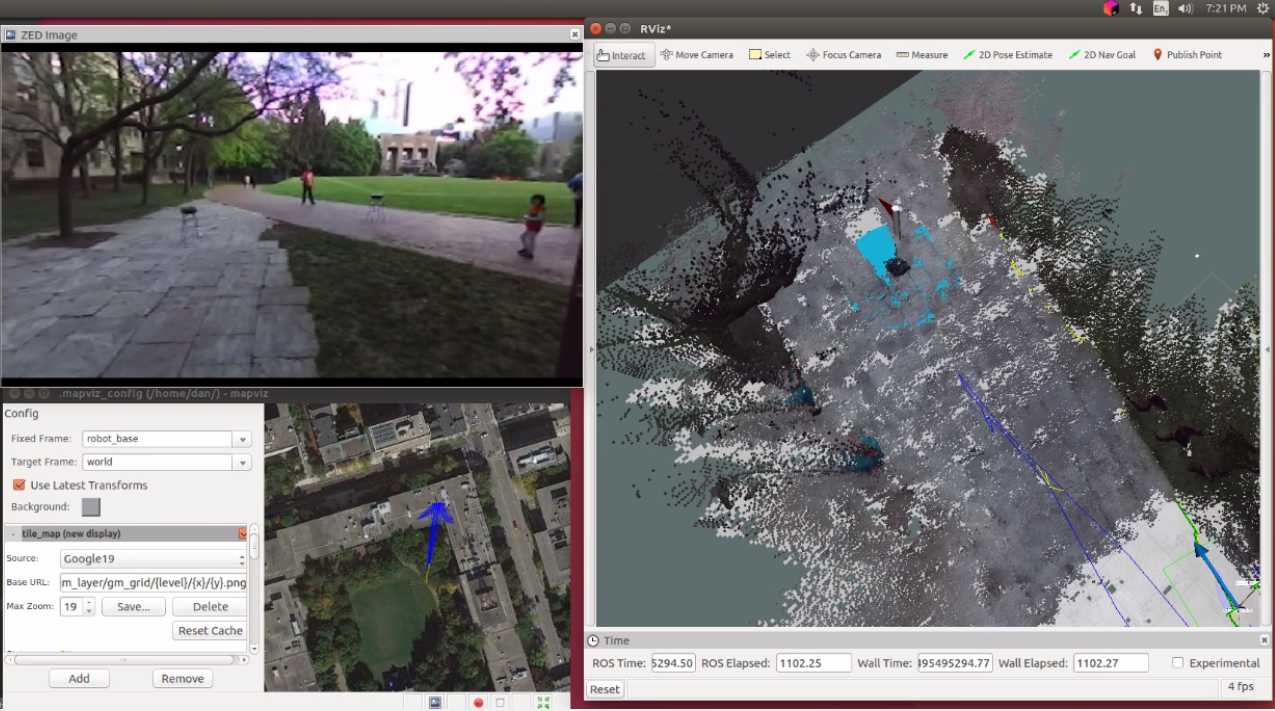
\includegraphics[width=\textwidth]{autosoftware}
\caption{Screenshot of R3's autonomous system tests with RTAB-Map (video available on YouTube\protect\footnotemark)}
\label{fig:autosoftware}
\end{figure}

\footnotetext{Video of an autonomous navigation by Team R3 with RTAB-Map and the ZED stereo camera \url{https://www.youtube.com/watch?v=p_1nkSQS8HE}}

In the launch file seen in Listing \ref{lst:rtab} on lines 3-5 show configurations to reduce noisy detection of obstacles. If you set \texttt{MaxGroundAngle} to 180 degrees, this effectively disables obstacle detection, which can be both useful and dangerous.

RTAB-Map also performs loop closures. Loop closure is the problem of recognizing a previously-visited location and updates the beliefs accordingly\footnote{More information about loop closures \url{https://en.wikipedia.org/wiki/Simultaneous_localization_and_mapping#Loop_closure}}. When an image is matched to a previously-visited location, a loop closure is said to have occurred. At this point RTAP-Map will adjust the map to compensate for drift that occurred since the last time the location was visited. Lines 8-10 of listing \ref{lst:rtab} increase the likelihood of loop closures being detected.  
\begin{lstlisting}[language=XML,frame=single,basicstyle=\ttfamily\footnotesize,breaklines=true,captionpos=b,caption={Important settings for tuning the RTAB-Map 3D mapping ROS package.},label={lst:rtab}]
<launch>
    <node pkg="rtabmap_ros" name="rtabmap" type="rtabmap" output="screen">
        <!-- Improve obstacle detection -->
        <param name="Grid/MaxGroundAngle" value="110"/> <!-- Maximum angle between point's normal to ground's normal to label it as ground. Points with higher angle difference are considered as obstacles. Default: 45 -->
        <param name="grid_eroded" value="true"/> <!-- remove obstacles which touch 3 or more empty cells -->

        <!-- Improve loop closure chances -->
        <param name="RGBD/LoopClosureReextractFeatures" type="string" value="true"/> <!-- Extract features even if there are some already in the nodes, more loop closures will be accepted. Default: false -->
        <param name="Vis/MinInliers" type="string" value="10"/> <!-- Minimum feature correspondences to compute/accept the transformation. Default: 20 -->
        <param name="Vis/InlierDistance" type="string" value="0.15"/> <!-- Maximum distance for feature correspondences. Used by 3D->3D estimation approach (the default approach). Default: 0.1 -->
    </node>
</launch>
\end{lstlisting}

Team R3's main strategy for the autonomous task of URC 2017 was to:

1.  Build a SLAM map by teleoperating from the start gate all the way to the tennis ball objective (actually this could be an autonomous navigation attempt by using the GPS location of the tennis ball as the goal),
2.  then we would then put a flag\footnote{RViz flag tool \url{http://docs.ros.org/jade/api/rviz_plugin_tutorials/html/tool_plugin_tutorial.html}} in RViz to mark where we observed the tennis ball,
3.  and then we would teleoperate back to the start gate,
4.  and complete a loop closure to correct for drift,
5.  and then use RViz to set an autonomous goal for where we saw the tennis ball.


\subsection{move\_base Path Planning}
The ROS navigation stack\footnote{ROS Navigation Stack \url{http://wiki.ros.org/navigation}}, also known as move\_base\footnote{Team R3's move\_base configuration file \url{https://github.com/teamr3/URC/blob/master/rosws/src/rover_navigation/launch/move_base.launch}}, is a collection of components/plugins that are selected and configured by YAML configuration files as seen in Listing \ref{lst:move_base}. For global path planning, the NavFn plugin is used which implements Dijkstra's shortest path algorithm.

\begin{lstlisting}[language=XML,frame=single,basicstyle=\ttfamily\footnotesize,breaklines=true,captionpos=b,label={lst:move_base},caption={move\_base is configured by independent YAML files that configure the subcomponents of move\_base.}]
<launch>
    <node pkg="move_base" type="move_base" name="move_base" output="screen" clear_params="true">
        <rosparam file="$(find rover)/costmap_common_params.yaml" command="load" ns="global_costmap"/>
        <rosparam file="$(find rover)/costmap_common_params.yaml" command="load" ns="local_costmap"/>
        <rosparam file="$(find rover)/local_costmap_params.yaml" command="load"/>
        <rosparam file="$(find rover)/global_costmap_params.yaml" command="load"/>
        <rosparam file="$(find rover)/base_local_planner_params.yaml" command="load"/>
    </node>
</launch>
\end{lstlisting}


The most interesting configuration file for move\_base is the base\_local\_planner\_params.yaml\footnote{Team R3's config file for base\_local\_planner\_params.yaml configuration of move\_base \url{https://github.com/teamr3/URC/blob/master/rosws/src/rover_navigation/config/base_local_planner_params.yaml}}. Given a path for the robot to follow and a costmap, the base\_local\_planner\footnote{Documentation for base\_local\_planner \url{http://wiki.ros.org/base_local_planner}} produces velocity commands to send to a mobile base. This configuration is where you set minimum and maximum velocities and accelerations for your robot, as well as goal tolerance. Make sure that the minimum velocity multiplied by the sim\_period is less than twice the tolerance on a goal. Otherwise, the robot will prefer to rotate in place just outside of range of its target position rather than moving towards the goal.

\begin{lstlisting}[language=yaml,frame=single,basicstyle=\ttfamily\footnotesize,breaklines=true,captionpos=b,caption={Important velocity settings in the base\_local\_planner\_params.yaml configuration file of move\_base.}]
TrajectoryPlannerROS:
  acc_lim_x:  0.5
  acc_lim_y:  0.5
  acc_lim_theta: 1.00

  max_vel_x:  0.27
  min_vel_x:  0.20
  max_rotational_vel: 0.4
  min_in_place_vel_theta: 0.27
  max_vel_theta: 0.1
  min_vel_theta: -0.1
  escape_vel: -0.19

  xy_goal_tolerance: 1
  yaw_goal_tolerance: 1.39626 # 80 degrees

  holonomic_robot: false
  sim_time: 1.7 # set between 1 and 2. The higher he value, the smoother the path (though more samples would be required)
\end{lstlisting}

\section{Tutorial: MapViz Robot Visualization Tool}\label{mapviz}

\begin{figure}
\centering
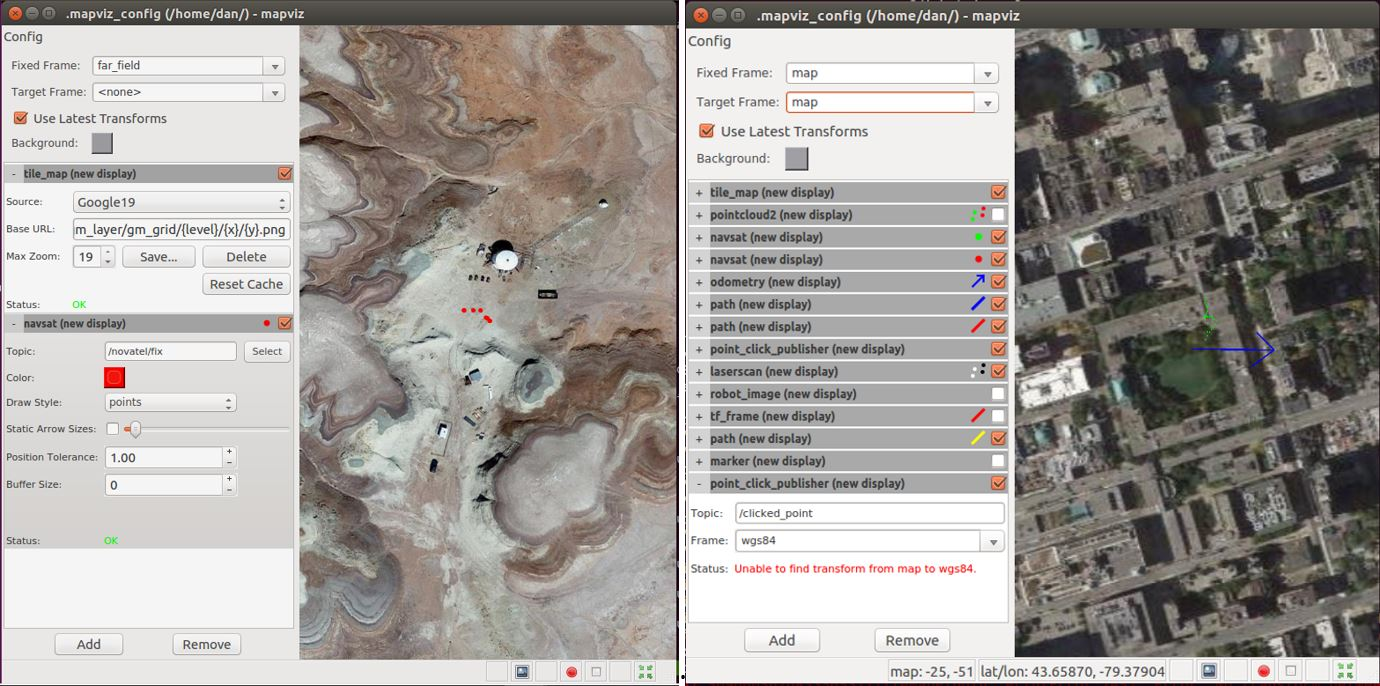
\includegraphics[width=\textwidth]{mapviz}
\caption{Screenshots of MapViz ROS visualization tool. Red dots indicate gps coordinates. Many more visualization layers are possible.}
\label{fig:mapviz}
\end{figure}


At the URC competition, Team R3 (Ryerson University) improved their situational awareness by using MapViz\footnote{Documentation and source code for MapViz \url{https://github.com/swri-robotics/mapviz}}. Mapviz is a ROS-based visualization tool with a plug-in system similar to rviz but focused only on a top down, 2D view of data. Any 3D data is flatening into the 2D view of MapViz. Created by the Southwest Research Institute in Florida for their outdoor autonomous robotics research, it is still under active open source development at the time of writing in December 2017. Using a plugin called tile-map, Google Maps satellite view can be viewed in MapViz Tile Map plugin.

The authors have contributed a Docker container\footnote{Docker container for proxying Google Maps to MapViz\url{https://github.com/danielsnider/MapViz-Tile-Map-Google-Maps-Satellite}} to make displaying Google Maps in MapViz as easy as possible. This container run software called MapProxy and which converts from the format of Google Maps API to a standard format called Web Map Tile Service (WMTS) which MapViz Tile Map plugin can display. The authors have set MapProxy's configuration\footnote{MapProxy config file \url{https://github.com/danielsnider/docker-mapproxy-googlemaps/blob/master/mapproxy.yaml}} to cache any maps that you load to \texttt{{\raise.17ex\hbox{$\scriptstyle\sim$}}/mapproxy/cache\_data/} so that they are available offline.


\begin{figure}
\centering
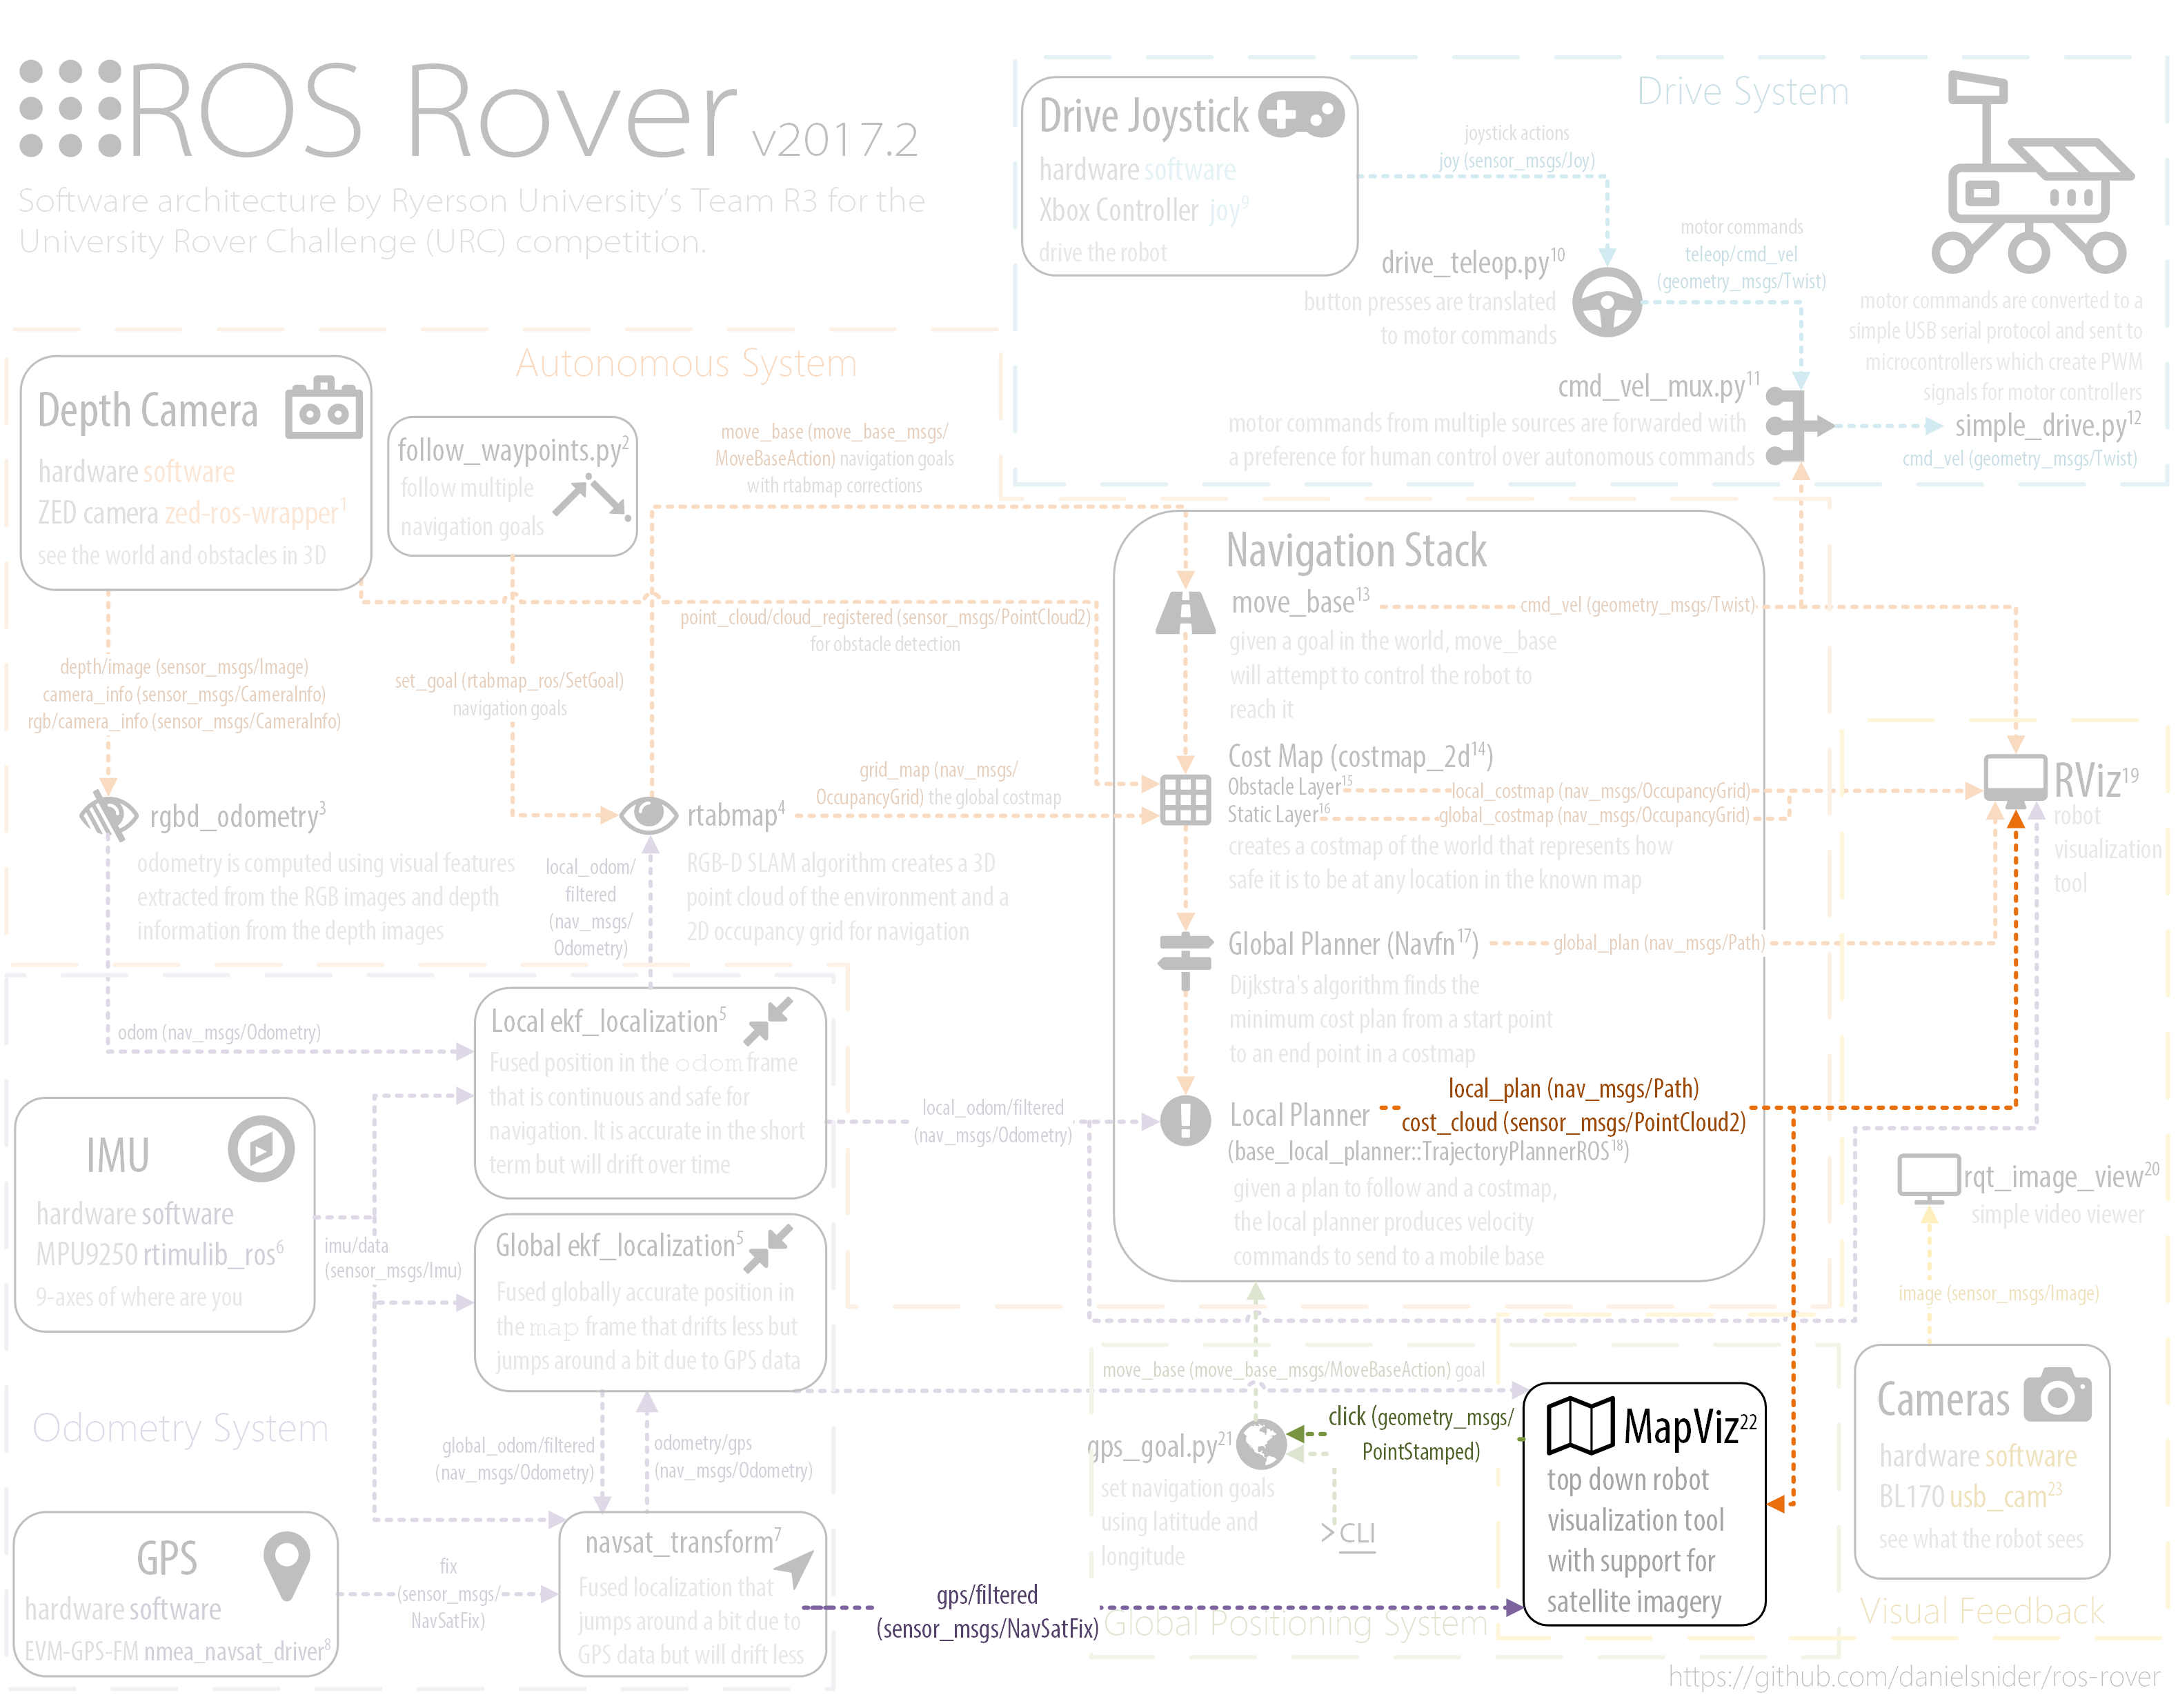
\includegraphics[width=\textwidth]{Mapviz_Diagram}
\caption{MapViz ROS node seen within Team R3's rover system. See fig. \ref{fig:Diagram} for the full diagram.}
\label{fig:Mapviz_Diagram}
\end{figure}

\subsection{Usage Instructions}
The goal of this tutorial is to install and configure MapViz to display Google Maps.

\noindent 1. Install mapviz, the plugin extension software, and the plugin for supporting tile maps which is needed to display Google Maps:

\begin{lstlisting}[frame=single,basicstyle=\ttfamily\footnotesize,breaklines=true]
$ sudo apt-get install ros-kinetic-mapviz ros-kinetic-mapviz-plugins ros-kinetic-tile-map
\end{lstlisting}

\noindent 2. Launch the MapViz GUI application:

\begin{lstlisting}[frame=single,basicstyle=\ttfamily\footnotesize,breaklines=true]
$ roslaunch mapviz mapviz.launch
\end{lstlisting}

\noindent 3. Using Docker to setup a proxy of the Google Maps API so that it can be cached and received by MapViz in WMTS format. To make this as simple as possible, run the Docker container created by the authors:

\begin{lstlisting}[frame=single,basicstyle=\ttfamily\footnotesize,breaklines=true]
$ sudo docker run -p 8080:8080 -d -t -v ~/mapproxy:/mapproxy danielsnider/mapproxy
\end{lstlisting}

The \texttt{-–v {\raise.17ex\hbox{$\scriptstyle\sim$}}/mapproxy:/mapproxy} option is a shared volume, a folder that it synced between the Docker container and the host computer. The \texttt{{\raise.17ex\hbox{$\scriptstyle\sim$}}/mapproxy} folder needs to be created, though it could be another location. The \texttt{-–t} option allocates a pseudo-tty which gives the program a terminal environment to run in. It is needed for most programs. The \texttt{-–p} option sets the Docker port mapping between host and container.

\noindent 4. Confirm MapProxy is working by browsing to \url{http://127.0.0.1:8080/demo/}. The MapProxy logo will be displayed and you can click on "Image-format png" to get an interactive map. Also, test that the first map tile is working by browsing to \url{http://localhost:8080/wmts/gm_layer/gm_grid/0/0/0.png}.

\noindent 5. In the MapViz GUI, click the "Add" button and add a new map\_tile display component.

\noindent 6. In the "Source" dropdown select "Custom WMTS Source...".

\noindent 7. In the "Base URL:" field enter the following: \url{http://localhost:8080/wmts/gm_layer/gm_grid/{level}/{x}/{y}.png}

\noindent 8. In the "Max Zoom:" field enter 19 and Click "Save...". This will permit MapViz to zoom in on the map 19 times. 

Google Maps will now display in MapViz. To set a default location in the world to display at program start up time, you can edit \texttt{{\raise.17ex\hbox{$\scriptstyle\sim$}}/.mapviz\_config}.

\begin{lstlisting}[frame=single,basicstyle=\ttfamily\footnotesize,breaklines=true,caption={MapViz setting for default viewing location (within a ROS frame) when GUI opens.},captionpos=b]
$ vim ~/.mapviz_config 
# edit the following lines
offset_x: 1181506
offset_y: -992564.2
\end{lstlisting}


\section{Tutorial: Effective Robot Administration}\label{administration}

In this tutorial, Team R3 (Ryerson University) shares two favorite preferences for making command line administration of ROS robots easier both for the URC competition and any other use case.



\subsection{tmux Terminal Multiplexer}

Tmux\footnote{Homepage for Tmux the terminal multiplexer \url{https://github.com/tmux/tmux/wiki}} is a popular linux command line program that can take over one terminal window and organize many terminals into grouped layouts and will continue running when you close the parent window or lose an SSH connection. Multiple people can join a tmux session to share an identical terminal view of a Linux system. Many technology professionals (especially linux and IT professionals) see tmux as essential to their workflow\footnote{A crash course to learn tmux \url{https://robots.thoughtbot.com/a-tmux-crash-course}}.

Tmux works harmoniously with ROS's modular design. Separate tmux windows can display different ROS components. Almost any ROS component can be launched, controlled, and debugged using ROS's command line tools. Using tmuxinator\footnote{Tmuxinator is an tool for tmux that lets to write tmux layout configuration files for repeatable layounts \url{https://github.com/tmuxinator/tmuxinator}}, you can codify the launching and debugging commands that you most often use into a repeatable layout.

At URC 2017, Team R3 used tmuxinator to launch all our robot's software systems. There was a section that contained the terminals running the drive software, another section with terminals running the arm software, another for the IMU, for the GPS, for the cameras, etc. All of it in an organized way. Just about every software can be started on the command line using tmuxinator after the rover's computer boots.

The tmuxinator configuration used by Team R3 was split into two sides: the robot config\footnote{The tmuxinator config used by Team R3 to start all the rover software components \url{https://github.com/teamr3/URC/blob/master/.tmuxinator.yml}}, and the base station config\footnote{The tmuxinator config used by Team R3 to start all the base station software components \url{https://github.com/teamr3/URC/blob/master/devstuff/dan/.tmuxinator.yml}}. The robot configuration launches all of the rover's software. The base station configuration launches all of the software needed to visualize and control the robot remotely by the teleoperator.


\begin{figure}
\centering
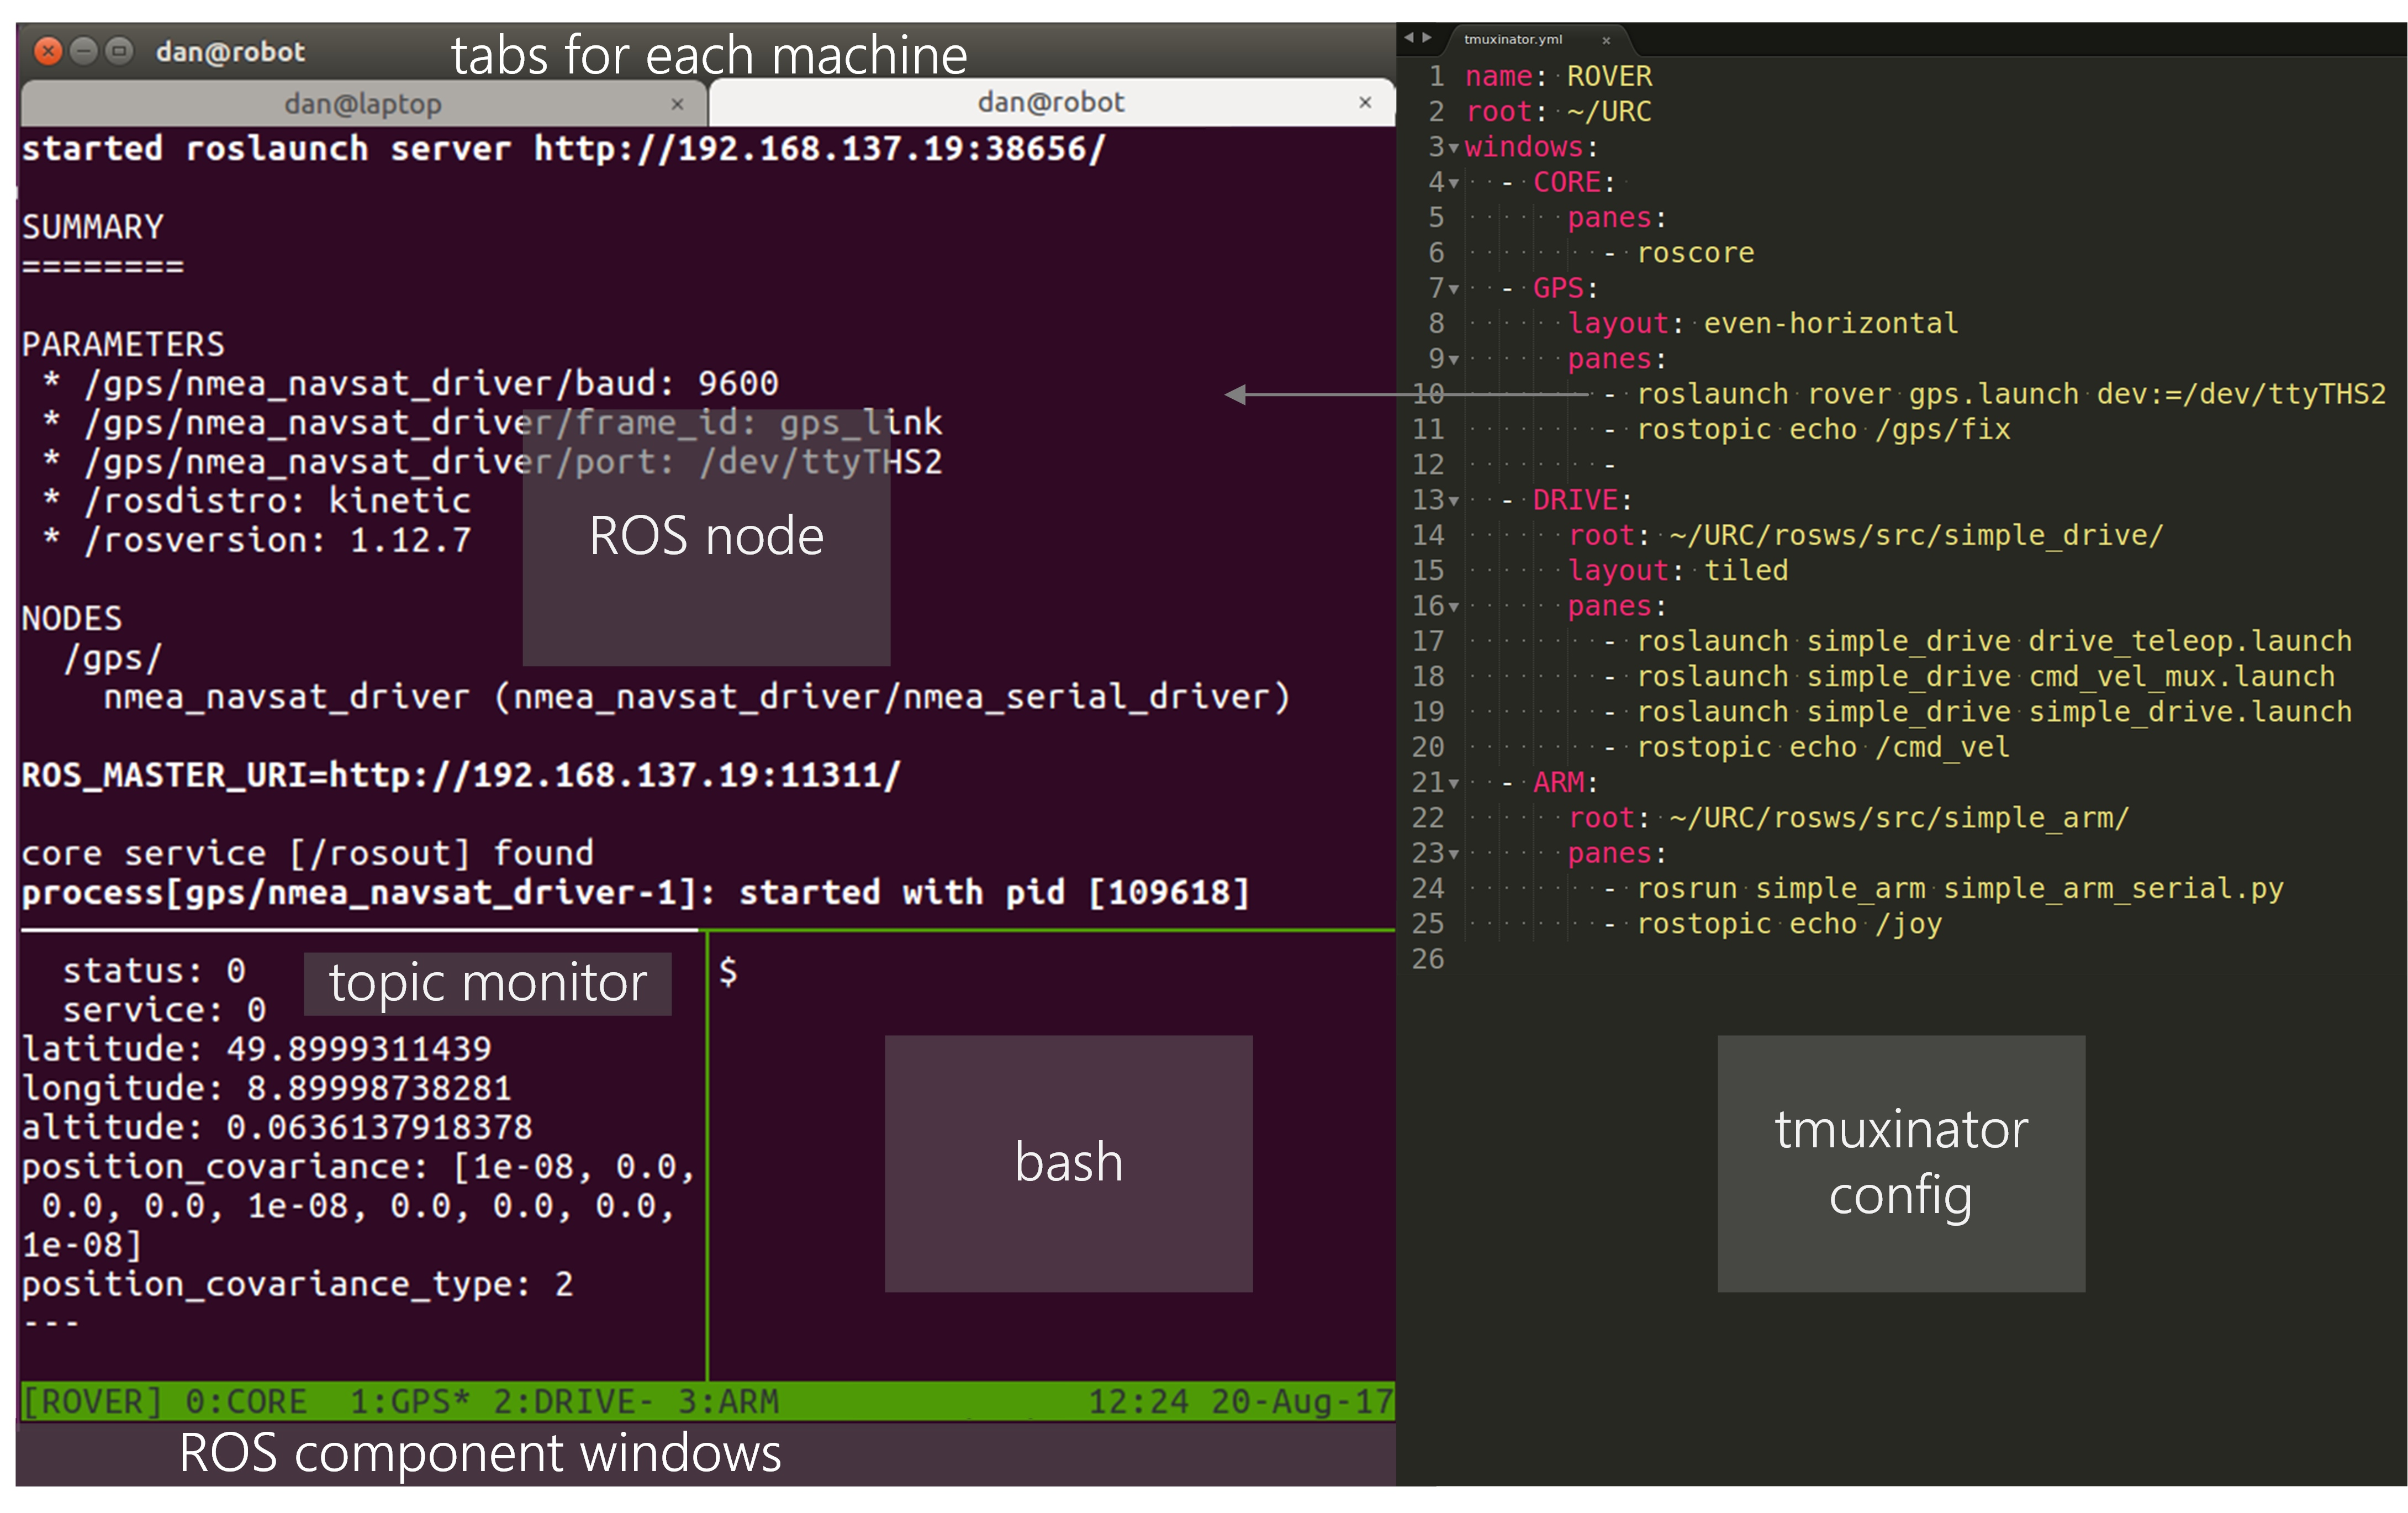
\includegraphics[width=\textwidth]{tmux}
\caption{An annotated example of tmuxinator's usefulness for ROS.}
\label{fig:tmux}
\end{figure}

Using Tmuxinator can be thought of as is a quick way to create a very simple user interface to help administer a robot (but it is not a replacement for Rviz and other existing tools). Building a robot GUI as a web interface or desktop application can be useful for some applications and novices who are unwilling to learn common command line tools, but such a GUI will require a lot more "plumbing" and "glue code" to create.

An implementation imperfection is that tmuxinator starts all of its panes (i.e. terminals) at the same time, running multiple roslaunch instances may try and fail to create multiple masters. The solution we implemented was to run a roscore separately, which has the added benefit of being able to stop and start roslaunches without worrying about which one is running the master. This still has the problem of roslaunches starting before the roscore though, so to solve this naively we have used a small wait time, for example "sleep 3; roslaunch..." in our tmuxinator config.

\subsection{ROS Master Helper Script}

Team R3 has developed a script\footnote{Team R3's ROS master helper script \url{https://gist.github.com/danielsnider/13aa8c21e4fb12621b7d8ba59a762e75}} to make it a little easier to connect your computer to a remote master that is not on your machine. The script when run will automatically set bash environment variables needed for ROS networking to work in a convenient way. The script will detect if your robot is online using ping (using a static IP for your robot) and set your ROS\_MASTER\_URI environment variable to point to your robot. If your robot is not online your own computer's IP will be used for your ROS\_MASTER\_URI, assuming you will do local or simulation development since you are away from your robot. To use this script run \texttt{source set\_robot\_as\_ROS\_master.sh} or add it to your \texttt{{\raise.17ex\hbox{$\scriptstyle\sim$}}/.bashrc}. Also, the script sets your own machine's ROS\_IP environment variable because it is needed in any case for ROS networking.

\section{Conclusion}\label{conclusion}

This chapter presented an overview of rover systems through the lenses of the University Rover Competition. Design summaries of 8 URC teams were surveyed and implementation details from 3 URC teams were discussed in a series of tutorials. Several new ROS packages were documented with examples, installation and usage instructions along with implementation details.

To summarize the main findings in this chapter: Rovers can be built by integrating existing software as thanks to the ROS ecosystem. The URC competition is very challenging and students learned a lot by participating. A variety of creative rover designs exist and the best rover teams were the most prepared and practiced.

We hope this chapter spurs greater collaboration between teams. Ideally, the teams of URC will look past the competitive nature of the event and view collaborating and building better robots as the more important goal. Building on a common core frees up time to focus on the hardest parts. Here are a few ways to further collaboration: 1) Contribute to a ROS package or the ROS core. 2) Open an issue, feature request, or pull request. 3) Discuss URC on the URC Hub forum. 4) Discuss ROS on their forum. 5) Contribute to a book like this.



\subsubsection*{Acknowledgments} We thank our advisor Professor Michael R. M. Jenkin P.Eng., Professor of Electrical Engineering and Computer Science, York University, NSERC Canadian Field Robotics Network. We also thank and appreciate the contributions of our survey respondents: Khalil Estell from San Jose State University, SJSU Robotics, and Jacob Glueck from Cornell University, Cornell Mars Rover, and Hunter D. Goldstein from Cornell University, Cornell Mars Rover, and Akshit Kumar from Indian Institute of Technology, Madras, Team Anveshak, and Jerry Li from University of Waterloo, UWRT, and Gabe Casciano from Ryerson University, Team R3, and Jonathan Boyson from Missouri University of Science and Technology (Missouri S\&T), Mars Rover Design Team.

\printbibliography

\section*{Authors Biographies}

\subsubsection*{Daniel Snider} received a bachelor of information technology (BIT) from the University of Ontario Institute of Technology in Ontario, Canada (2013). He is currently a member of the R3 robotics team at Ryerson University and works as a computer vision software developer at SickKids Research Institute, associated with the University of Toronto. His current research is on the design of modular polyglot frameworks (such as ROS) and scientific workflow systems.

\subsubsection*{Matthew Mirvish} is currently a student at Bloor Collegiate Institute. He is also currently a member of the R3 robotics team at Ryerson University and helps write the code for their rover for URC. He mainly specializes in the autonomous task, but usually ends up helping with anything he can get his hands on. In his spare time he dabbles with microcontrollers as well as creating small computer games.

\subsubsection*{Michal Barcis} received a bachelor's and master's degree in computer science from University of Wroclaw, Poland, in 2015 and 2016, respectively. He is currently pursuing the Ph.D. degree as a researcher with the Alpen-Adria-Universitat Klagenfurt, Austria. Between 2015 and 2017 he was a member of the Continuum Student Research Group at the University of Wroclaw. His research interests include robotics, computer networks and machine learning.

\subsubsection*{Vatan Aksoy Tezer} is currently studying Aerospace Engineering in Istanbul Technical University, Turkey. He was the software sub-team leader of ITU Rover Team during 2016-2017 semester and worked on autonomous navigation, communication, computer vision and high level control algorithms. He previously worked on underwater robots, rovers and UAVs. He is currently conducting research on navigation in GPS denied environments using ROS.

 
\end{document}

\begin{figure}
\centering
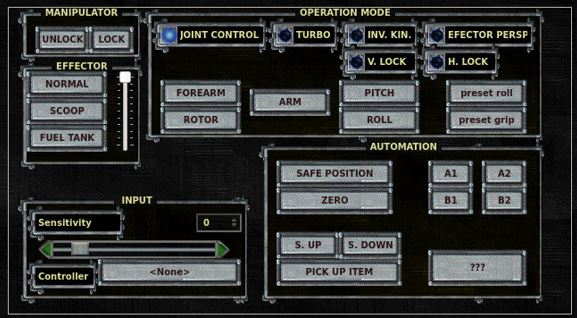
\includegraphics[width=\textwidth]{continuumGUI3}
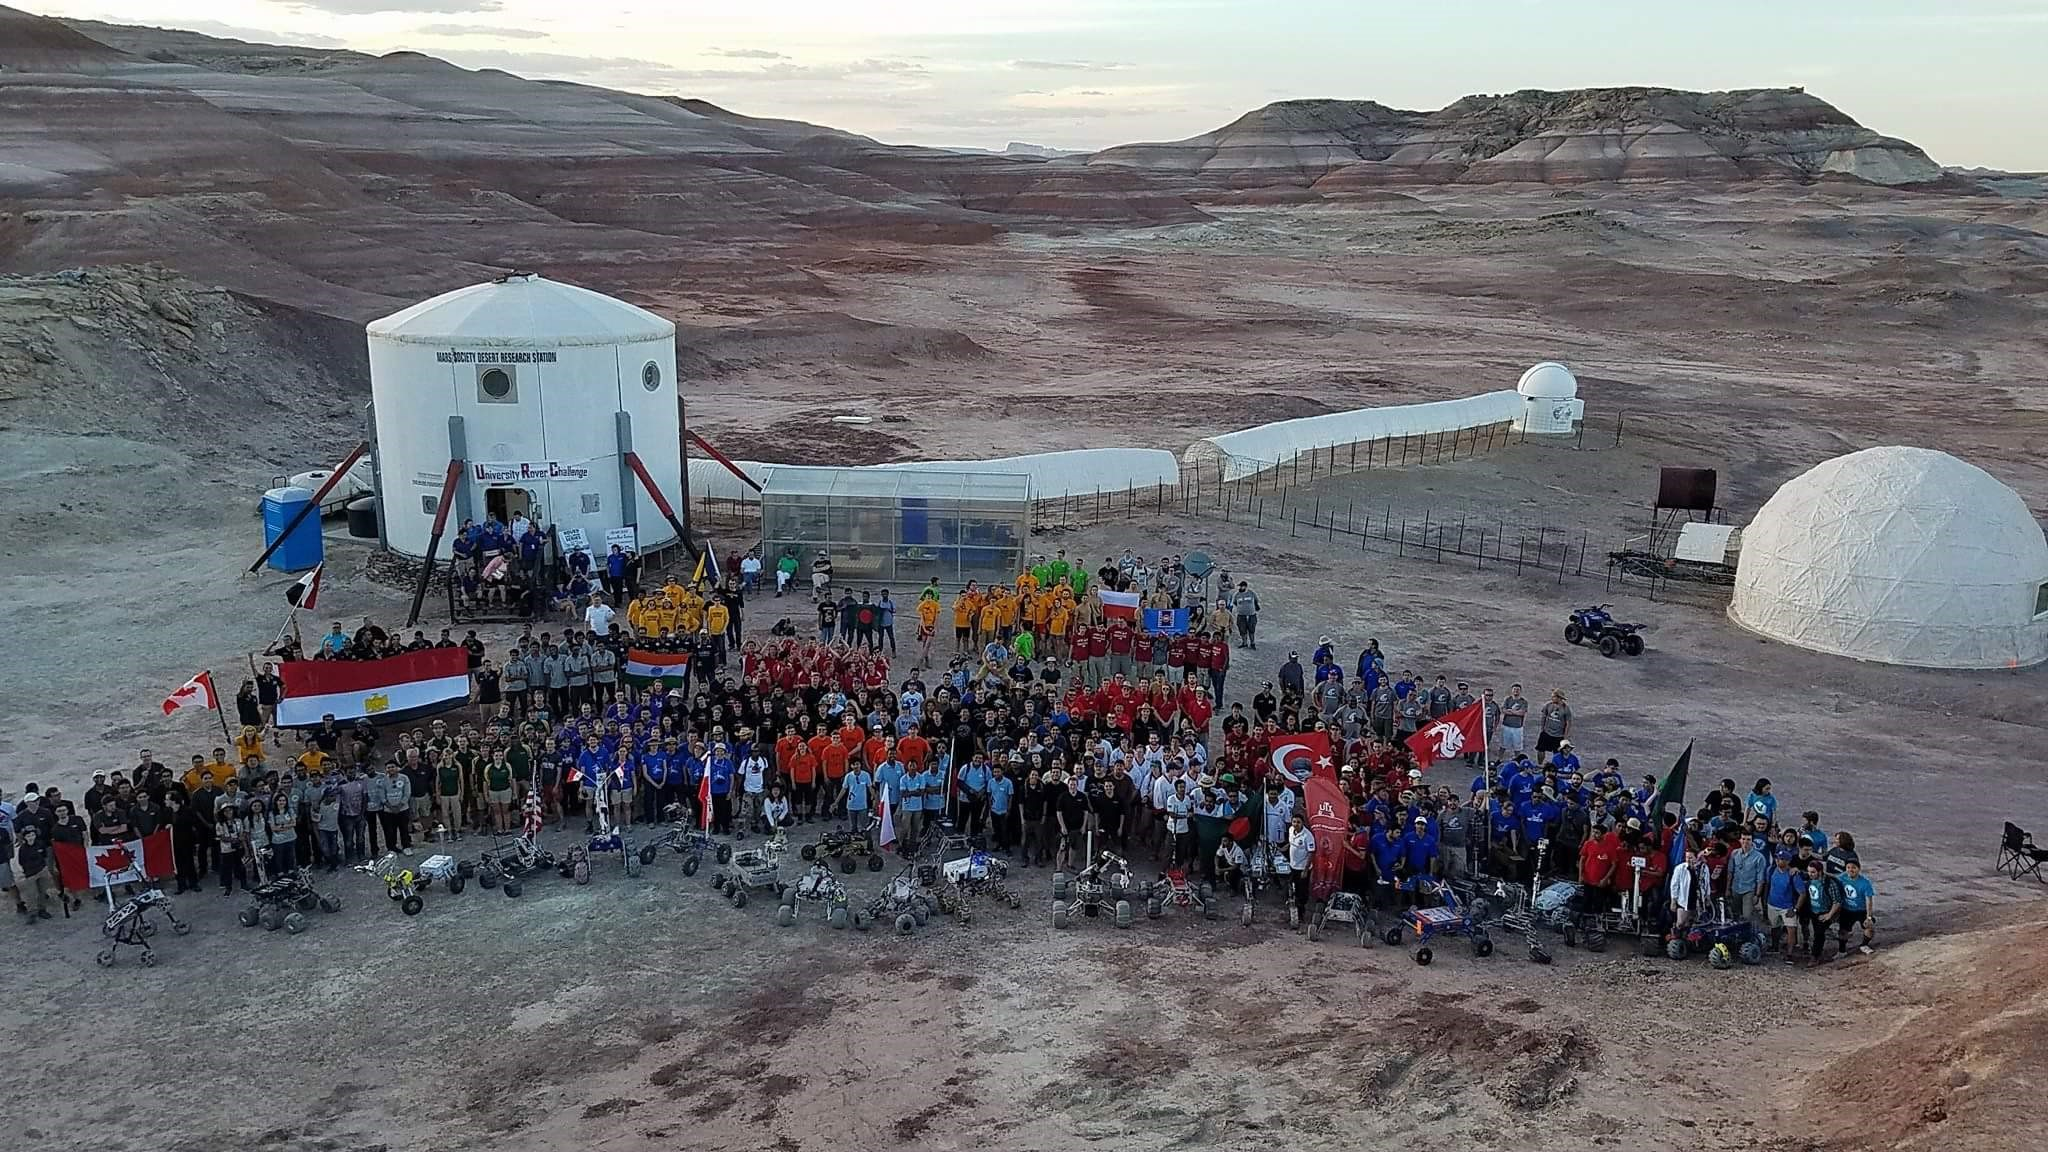
\includegraphics[height=6.2cm]{group_photo}
\caption{Group photo of URC 2017 finalists at the Mars Desert Research Station in Utah.}
\label{fig:group_photo}  
\end{figure}


\begin{lstlisting}[frame=single,caption={My Caption},captionpos=b,numbers=left]  

\begin{lstlisting}[frame=single,caption={My Caption},captionpos=b,numbers=left,keywordstyle=\color{blue}\bfseries,basicstyle=\ttfamily\small, language=Python]  % Start your code-block

[frame=single,basicstyle=\ttfamily\scriptsize,breaklines=true] 